

\documentclass{bredele}
%\usepackage{natbib}
\usepackage{amsmath,amssymb,amsfonts,latexsym,cancel}
\usepackage{amssymb}
\usepackage{graphicx}
\usepackage{natbib}        % required for bibliography
\usepackage{caption}
\usepackage{subcaption}
\usepackage{here}
\usepackage{geometry}
\usepackage{dblfloatfix}
\usepackage{gensymb}
\usepackage{float}
\usepackage{wrapfig}
\usepackage{color}
\usepackage{colortbl}
\usepackage{multirow}
\usepackage{booktabs}
\usepackage{pgfplots}
\usepackage{multicol}
\usepackage{kantlipsum} % for the mock text
\usepackage{textcomp}
\usepackage{titlesec}
\usepackage{url}

%\setcounter{secnumdepth}{4}

\setlength{\columnsep}{0.5cm}

\def\refname{References}

\newcommand{\includegraphicsSchema}[1]{\includegraphics[width=0.8\columnwidth]{figures/#1}}
\newcommand{\includegraphicsSimu}[1]{\includegraphics[width=\columnwidth]{figures/#1}}

\newcommand{\sect}[1]{section~\ref{#1}}
\newcommand{\subsect}[1]{subsection~\ref{#1}}

\newcommand{\fig}[1]{Fig.~\ref{#1}}
\newcommand{\eqn}[1]{(\ref{#1})}

\newtheorem{theorem}{Theorem}[section]
\newtheorem{definition}[theorem]{Definition}
\newtheorem{lemma}[theorem]{Lemma}
\newtheorem{remark}[theorem]{Remark}
\newtheorem{proof}[theorem]{Proof}

\title{Teleoperation et Navigation}

\discipline{Automatique-Productique}

\dirdethese{Nicolas Marchand}
\codirdethese{Jos\'{e} Ernesto Gomez Balderas}
\cocodirdethese{Pedro Casillo}
\cocodirdethese{Amaury Negre}

\titredudirdethese{CNRS}

\jury{
\begin{description}
% \item[Rapporteur:] \textsc{Antonio FRANCHI}, Charg\'{e} de recherche, LAAS-CNRS, Toulouse,
% \item[Rapporteur:] \textsc{Arturo ZAVALA RIO}, Charg\'{e} de recherche, Instituto Potosino de Investigación Científica y Tecnológica, A.C., S.L.P, Mexique,
% \item[Examinateur:] \textsc{St\'{e}phan VIOLLET}, Directeur de recherche, ISM-CNRS, Marseille,
% \item[Examinateur:] \textsc{Edouard LAROCHE}, Professeur, ICube - AVR, Strasbourg,
% \item[Examinateur:] \textsc{Ahmad HABLY}, Ma\^{i}tre de conf\'{e}rences, GIPSA-Lab-CNRS, Grenoble.
\end{description}
}

\author{Jos\'{e} Juan T\'{e}llez Guzm\'{a}n}

\date{\today}

\nomdeuniversite{Universit\'{e} de Grenoble}
\logouniversite{figures/uga_logo_visuel} %nom du fichier
\scalelogouniversite{0.24} % mise a l'echelle de l'image (0.5=50% par exemple)
\logolabo{figures/GIPSA-lab_logo}
\scalelogolabo{0.4}

\unite{Automatique}
\ecoledoc{\'{E}lectronique, \'{E}lectrotechnique, Automatique et Traitement du Signal (EEATS) }


\usepackage[a4paper]{meta-donnees}
\begin{document}


% la ligne ci-dessous est à insérer obligatoirement dans le préambule du document avant \begin{document}

% les lignes en bas sont à insérer obligatoirement après

%%%%%%%%%%%%%%%%%%%%%%%%%%%%%%%%%%%%%%%%%%%%%%%%%%%%%%
%%             Commandes Meta-données               %%
%%   à renseigner par les auteurs pour générer      %%
%%     la couverture modèle Univ. Grenoble          %%
%%%%%%%%%%%%%%%%%%%%%%%%%%%%%%%%%%%%%%%%%%%%%%%%%%%%%%
%%      Fichier encodé au format ISO-8859-16        %%

%\Sethpageshift{???mm}   %%optionnel : à décommenter si besoin pour ajout d'espace afin de center la couvérture horizontalement (valeur par défaut est -5.5mm)
%\Setvpageshift{???mm}   %%optionnel : à décommenter si besoin pour ajout d'espace afin de center la couvérture verticalement (valeur par défaut est -15.5mm)


% \Universite{Univsersit\'{e} de Grenoble}    %%optionnel : à décommenter et à renseigenr si vous voulez changer le non d'université
% \Grade{DOCTEUR DE L'UNIVERSIT\'{E} DE GRENOBLE}  %%optionnel : à décommenter et à renseigenr si vous voulez changer le grade
% \Specialite{Automatique - Productique}
% \Arrete{7 Ao\^ut 2006}
% \Auteur{Jonatan Uziel ALVAREZ MU\~{N}OZ}
% \Directeur{Nicolas MARCHAND,}
% \CoDirecteur{Jos\'{e} Fermi GUERRERO CASTELLANOS}
% \Coencadrent{Sylvain DURAND}%%optionnel : à décommenter et à renseigenr si présence d'un Co-directeur de thèse
% \Laboratoire{du GIPSA-Lab de Grenoble}
% \EcoleDoctorale{l'\'{e}cole doctorale EEATS}
% \Titre{Modelling and control of VTOL vehicles with rigid manipulators}
%\Soustitre{}      %%optionnel : à décommenter et à renseigenr si présence d'un sous-titre de thèse
% \Depot{}


% Commande pour création de nouvelles catégories dans le jury:

%\UGTNewJuryCategory{...NomDeLaCategorie...}{...Definition...}

% Exemple \UGTNewJuryCategory{UGTFamille}{Membre de la famille} que nous ajoutons dans la commande \Jury ci-dessous sous la forme \UGTFamille{Jean Rousseau}{(...titre_et_affiliation...s'il_y_en_a...)}


% \Jury{
% %\UGTPresident{...Civilité, Prénom-et-Nom...}{...titre-et-affiliation...}
% %\UGTPresidente{...Civilité, Prénom-et-Nom...}{...titre-et-affiliation...}
%
% \UGTRapporteur{Antonio FRANCHI}{Charg\'{e} de recherche, LAAS-CNRS, Toulouse}      %% 1er rapporteur
% \UGTRapporteur{Arturo ZAVALA RIOS}{Charg\'{e} de recherche, Instituto Potosino de Investigación Científica y Tecnológica, A.C., S.L.P, Mexique}      %% second rapporteur
%
% \UGTExaminateur{St\'{e}phane VIOLLET}{Directeur de recherche, ISM-CNRS, Marseille}     %% 1er examinateur
% \UGTExaminateur{Edouard LAROCHE}{Professeur, ICube - AVR, Strasbourg}     %% second examinateur
% %\UGTExaminatrice{Ahmad HABLY}{...titre-et-affiliation...}    %% 3ème examinateur
% \UGTExaminateur{Ahmad HABLY}{Ma\^{i}tre de conf\'{e}rences, GIPSA-Lab-CNRS, Grenoble}
% %\UGTInvitee{...Civilité, Prénom-et-Nom...}{...titre-et-affiliation...}
%
% \UGTDirecteur{Nicolas MARCHAND}{Directeur de Recherche, GIPSA-Lab-CNRS, Grenoble}       %% Directeur de thèse
% \UGTCoDirecteur{Jos\'{e} Fermi GUERRERO CASTELLANOS}{Professeur, BUAP, Puebla, Mexique}%% Co-Directeur de thèse s'il y en a
% \UGTCoDirecteur{Sylvain DURAND}{Ma\^{i}tre de conf\'{e}rences, INSA \& ICube, Strasbourg}%% Co-Directeur de thèse s'il y en a
%
% }

% \MakeUGthesePDG    %% très important pour générer la couvérture de thèse
%
%
%
% \maketitle


\clearemptydoublepage
\chapter*{Aknowledgments}
\thispagestyle{empty}

\clearemptydoublepage
\frontmatter


%\clearemptydoublepage
%\shorttableofcontents{Table of Contents}{0}
%\newpage
\clearemptydoublepage
\tableofcontents
\clearemptydoublepage
\listoffigures

\clearemptydoublepage
\mainmatter % Ne pas oublier, avec \frontmatter et \backmatter

%\chapter*{Introduction}
 \chaptermark{Introduction}
% \addcontentsline{toc}{chapter}{Introduction}\markboth{INTRODUCTION}{}
%\input{Chapter01/introduction.tex}

\clearemptydoublepage
%!TEX root = ../thesis.tex
%*******************************************************************************
%****************************** Second Chapter *********************************
%*******************************************************************************

\chapter{Preliminaries and state of the art}

\ifpdf
    \graphicspath{{Chapter2/Figs/Raster/}{Chapter2/Figs/PDF/}{Chapter2/Figs/}}
\else
    \graphicspath{{Chapter2/Figs/Vector/}{Chapter2/Figs/}}
\fi

In this chapter, some mathematical preliminaries that will be used throughout the document are presented. The first part is focused on the image processing. After it is explained the basic concepts of projective geometry, and it is made an analysis of the model geometry. Although this work considers that the intrinsic and extrinsic parameters are known, an introduction of the techniques of calibration of the camera is written in this part. In the second section of the chapter there is an overview of the mini-helicopter four-rotor UAVs, and in the same way the dynamic model is detailed.

 \section{Computer Vision}
 \subsection{Projective geometry}
 \subsection{Model geometry}
 \subsection{Camera calibration}
 \subsection{Formation of the image in projective geometry}



 \section{UAVs: Mini-helicopter of four rotors}

 An Unmanned Aerial Vehicle (UAV) is an autonomous flying machine, this means that the vehicle can perform flights without a human pilot by the usage of an autonomous pilot algorithm. While the concept of UAV seems a novelty, its usage is not. In fact, the interest in the study of these type of vehicles has increased, and there are many works published especially related to control laws applied on the topic. The research on this subject is also possible due to the evolution of information and communication technologies and the power computation of the different devices.

It should be noted that the ballistic or semi-ballistic missiles, the cruise missiles and the artillery projectiles are not considered UAV systems.

An UAV system is composed mainly by two elements:
\begin{itemize}
  \item Flight component: formed by the aerial vehicle.
  \item Ground component: formed by the ground station, which allows the communication between this and the aerial system, data processing, monitoring, control, etc.
\end{itemize}

In general the drones can be classified according with the size, the application or a combination of both, however, the size is the most used criterion to make the classification. The classification, depicted in \fig{fig:categories} is resumed in the next items, \cite{phdguerrero:2008}:
\begin{itemize}
  \item Micro-UAV: This kind of vehicles can be operated by just one person. The propulsion is electrically made and due to the low cost of the materials, the vehicles are primarily used for civilian applications. The average autonomy is about 30 minutes.
  \item Mini-UAV: The equipment necessary for these vehicles is more specialized. In general, these drones fly at speeds of $70km/h$ and medium altitudes of $3,5km$. Their size allows them to fly around 4 hours.
  \item MALE/HALE: The Medium Altitude High Endurance (MALE) drones are used to perform higher endurance flights and also at higher altitudes ($10-15km$). The High Altitude High Endurance (HALE) drones can fly at about $20km$ of altitude. These drones are able to perform missions with medium endurance of two days. The Predator (MALE) and the Global Hawk (HALE) are the most popular drones of this category and are mainly applied for military missions.
  \item UCAV: The Unmanned Combat Air Vehicle is mainly used for offensive missions. They are under research and only some prototypes are available, like the RQ-170 Centinel.
\end{itemize}


\begin{figure}[H]
    \centering
    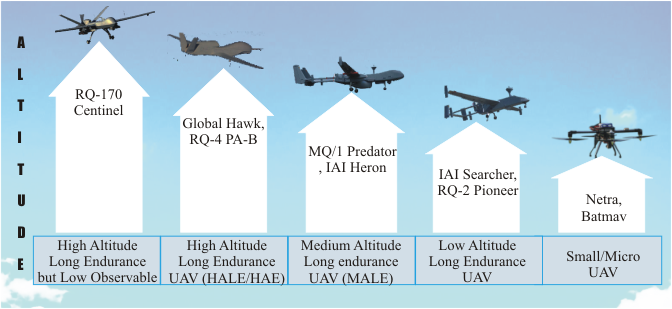
\includegraphics[width =\textwidth]{figures/categories.png}
    \caption{The different categories of drones.}
    \label{fig:categories}
  \end{figure}

Due to their aerodynamical function, there is an alternative classification, where it is possible to find three families: fixed wings aircrafts, rotating wings aircrafts and the swing-wing aircrafts. A study shows that the research has mainly focused on the rotating wings aircrafts with VTOL (Vertical Take Off and Landing) configuration. These vehicles are capable of take off and land in a vertical way and due to this advantage, the range of applications is very extensive, being used on military and civilian applications, like surveillance, rescue, aerial mapping, etc.

 \subsection{Vertical Take Off and Landing (VTOL) vehicles}
 \subsection{Rotorcraft}
\begin{itemize}
  \item Helicopter: is a type of rotorcraft in which lift and thrust are supplied by rotors. This allows the helicopter to take off and land vertically, to hover, and to fly forward and laterally. These attributes allow helicopters to be used in congested or isolated areas where fixed-wing aircrafts would usually not be able to take off or land.\fig{apache} shows an example of a helicopter.

      \begin{figure}[h!]
        \centering
        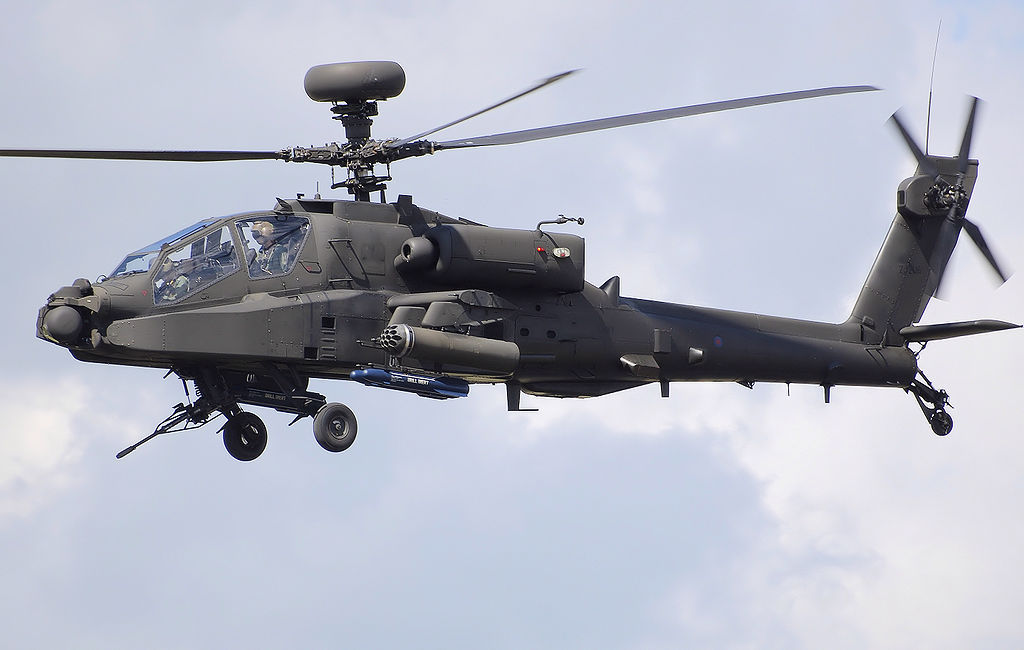
\includegraphics[width=0.4\textwidth]{figures/apache.jpg}
        \caption{An Apache attack helicopter}\label{apache}
      \end{figure}

  \item Multirotor: also called multicopter, is a rotorcraft with more than two rotors. An advantage of multirotor aircraft  is the simpler rotor mechanics required for flight control. Unlike single and double-rotor helicopters, multirotors often use fixed-pitch and yaw blades; control of vehicle motion is achieved by varying the relative speed of each rotor to change the thrust and torque produced by each one. Due to their ease of both construction and control, multirotor aircraft are frequently used in radio control aircraft and UAV projects, in which the names \textbf{tricopter}, \textbf{quadcopter} see \fig{fig:quaddji}, \textbf{hexacopter} and \textbf{octocopter} see \fig{fig:octodji}, are frequently used to refer to 3, 4, 6 and 8-rotor helicopters, respectively.
%
  \begin{figure} [h!]
\centering
% \begin{multicols}{2}
\begin{subfigure}[t]{0.45\textwidth}
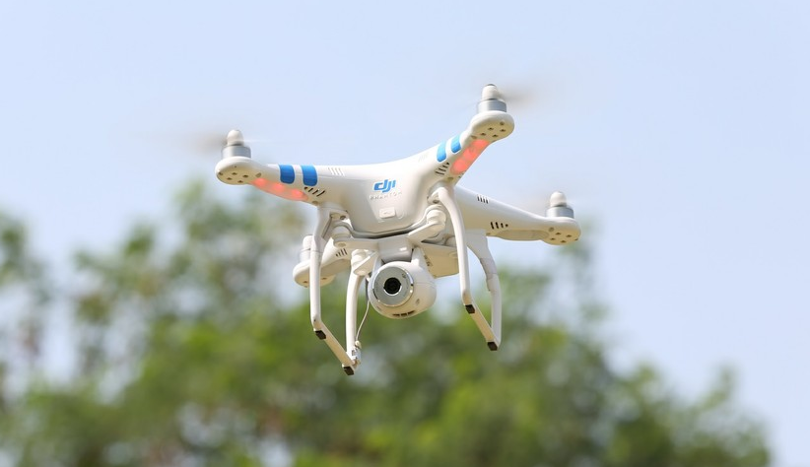
\includegraphics[width = \textwidth]{figures/quaddji.png}
\caption{}
\label{fig:quaddji}
\end{subfigure}
%$\qquad$
%\hfill
\begin{subfigure}[t]{0.45\textwidth}
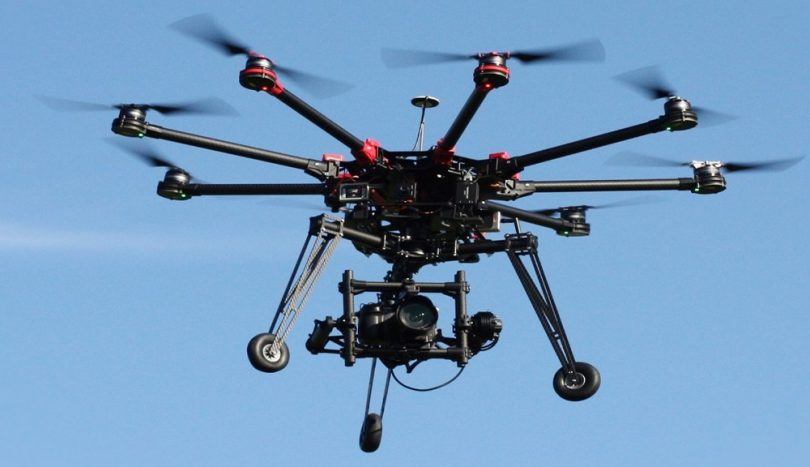
\includegraphics[width = \textwidth]{figures/octodji.jpg}
\caption{}
\label{fig:octodji}
\end{subfigure}
\caption{(a)Quadcopter and (b)octocopter configurations, courtesy of (\cite{website:dji})}
  \label{fig:multirotor}
\end{figure}

%
\item Autogyro: is also known as gyroplane, gyrocopter or rotaplane. Is a type of rotorcraft that uses an unpowered rotor in autorotation to develop lift, and an engine-powered propeller, similar to that of a fixed-wing aircraft, to provide thrust. While similar to a helicopter rotor in appearance, the autogyro's rotor must have air flowing through the rotor disc to generate rotation. \fig{auto} shows an example of an autogyro.

      \begin{figure}[h!]
        \centering
        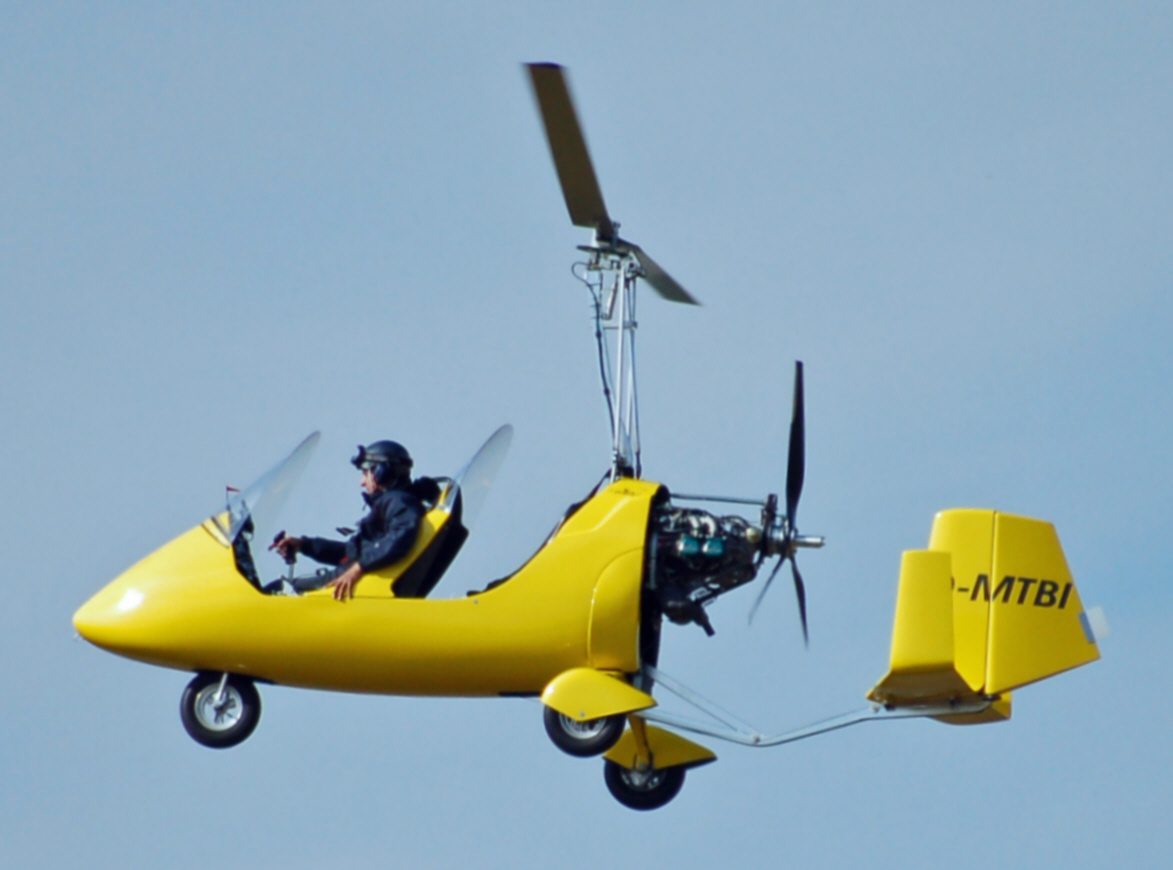
\includegraphics[width=0.4\textwidth]{figures/autogyro.jpg}
        \caption{Autogyro MT-03 in flight}\label{auto}
      \end{figure}

  \item Gyrodyne: is a type of VTOL aircraft with a helicopter rotor-like system that is driven by its engine for take off and landing and also includes one or more conventional propellers to provide forward thrust during cruising flight. Lift during forward flight is provided by a combination of the rotor, like the autogyro, as well as conventional wings.

   \fig{gyro} shows an example of gyrodyne.
      \begin{figure}[h!]
        \centering
        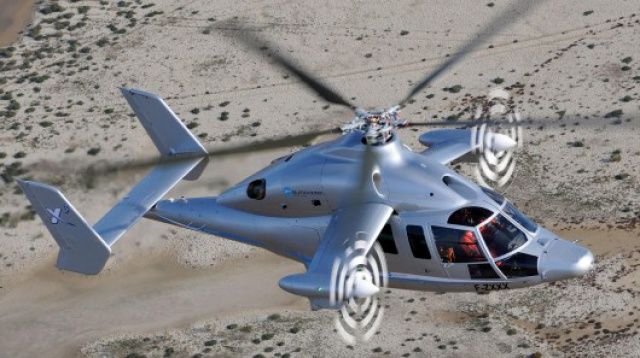
\includegraphics[width=0.45\textwidth]{figures/gyro.jpg}
        \caption{Gyrodyne AM-X3 in flight}\label{gyro}
      \end{figure}

\end{itemize}

\subsection{Powered lift}
\begin{itemize}
  \item Convertiplane: is an aircraft which uses rotor power for vertical take off and landing and converts to fixed-wing lift in normal flight. These vehicles may be divided into two broad classes, based on wether the rotor is fixed as in a helicopter or tilts to provide thrust in forward flight. \fig{convert} shows an example of a convertiplane.

      \begin{figure}[h!]
        \centering
        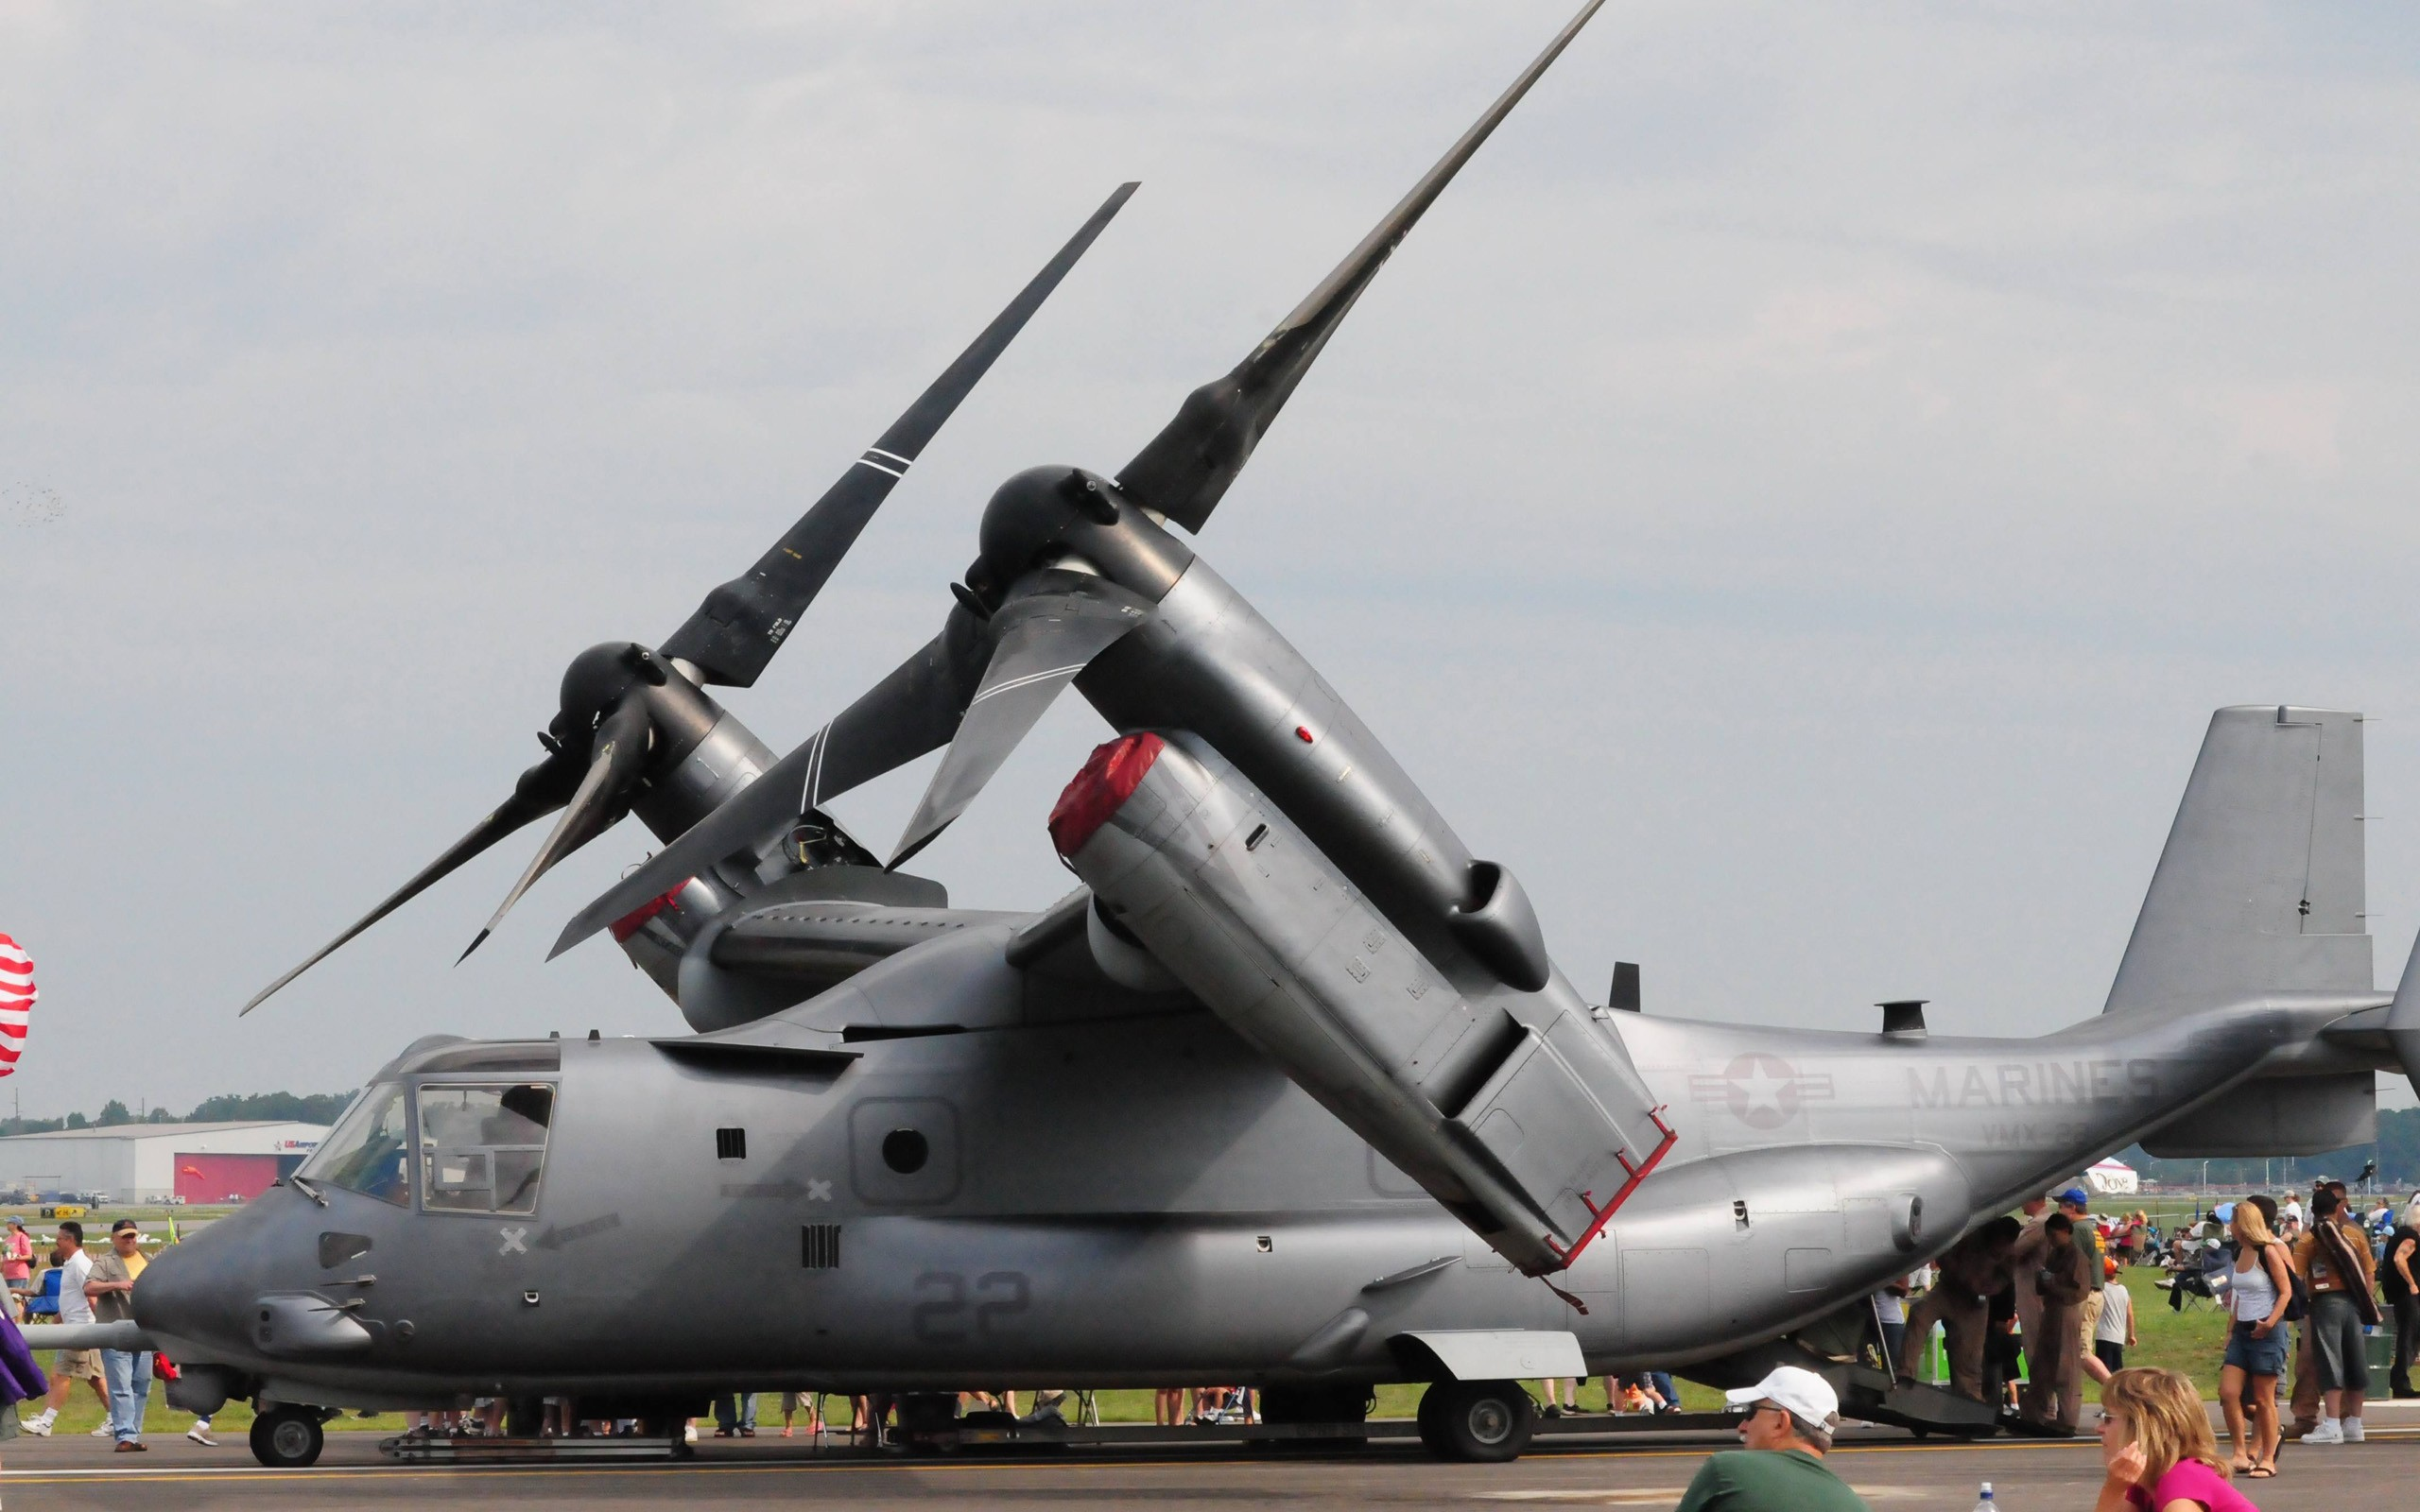
\includegraphics[width=0.4\textwidth]{figures/converti.jpg}
        \caption{Convertiplane}\label{convert}
      \end{figure}

  \item Tail-sitter: called also tailsitter, is a type of VTOL vehicle that takes off and lands on its tail, then tilts horizontally for forward flight. \fig{tail} shows an example of tail-sitter UAV's.

      \begin{figure}[h!]
        \centering
        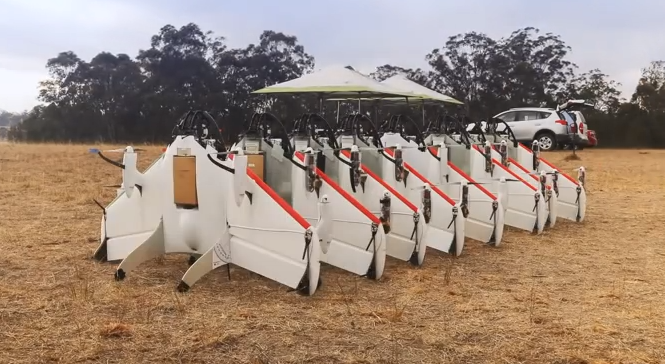
\includegraphics[width=0.45\textwidth]{figures/tail.png}
        \caption{Tail-sitter prototypes, as part of the Google’s project Wing for delivery}\label{tail}
      \end{figure}

  \item Lift jets: is an auxiliary jet engine used to provide lift for VTOL operation, but may be shut down for normal wing-borne flight.
  \item Lift fans: is an aircraft configuration in which lifting fans are located in large holes in an otherwise conventional fixed wing or fuselage. It is used for V/STOL \footnote{Vertical and/or Short Take-Off and Landing} operation. The aircraft takes off using the fans to provide lift, then transitions to fixed.wing lift in forward flight. Several experimental craft have been flown, but only the F-35 Lighting II entered into production, see \fig{f35}

      \begin{figure}[h!]
        \centering
        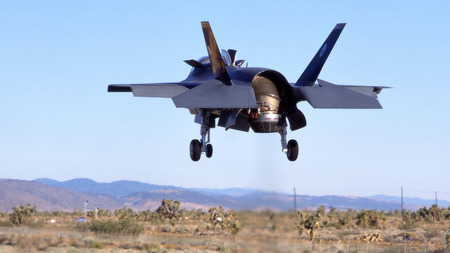
\includegraphics[width=0.45\textwidth]{figures/f35.jpg}
        \caption{F-35 Lighting II combat aircraft during take off}\label{f35}
      \end{figure}

\end{itemize}

The present work is centered on the analysis and study of multirotors, particularly on the modelling and control of a quadcopter carrying a manipulator arm. However, during the development of the project, the hexacopter configuration was also used. It allowed the obtention of some interesting results.

\section{Multi-rotors: state of the art}

The most common vehicle with the capacity of take off and landing in vertical way is the standard helicopter, which is composed of a principal rotor and a rear rotor. However, the multirotors, where we can find the four rotor helicopter, quadrotor or quadcopter, the hexacopter or hexarotor and the octocopter or octorotor have been the center of interest for many works in the last years, see \cite{Guerrero:2011}, \cite{Alaimo:2013} and \cite{Fogelberg:2008}. Some of the advantages offered by these vehicles are its symmetry, which makes it easy to design and build. The usage of four, six or eight rotors provides improved stability on hover, because the distributed pushing forces are acting at the same distance from the center of mass instead of just one pushing force acting on the whole center of mass. Also, the propellers can be protected by the frame of the prototype, which makes its usage indoor safer, face to the non-protected propellers of the standard helicopter.

The modeling of this kind of vehicles has done possible the design of many control laws which allow the attitude and position stabilization with good results. Some of the most used control laws have been: backstepping, found on \cite{Bouabdallah:2005}, \cite{Abdelaziz:2006} and \cite{Wu:2010}; sliding mode control has also been applied to these vehicles, and it can be found on \cite{Bouabdallah:2005}, \cite{Zheng:2014} and \cite{Arellano:2013}; linear control laws (PD and PID), they can be seen at \cite{erginer:2007}, \cite{li:2011} and \cite{hoffmann:2007}.

Other interesting projects developed with multi-rotors can be found on the domains of: navigation, where embedded cameras and/or different sensors are used to know the relative position of the aerial system, see \cite{courbon:2009} and \cite{sebesta:2012}; fault-tolerant control, where fault detection on the actuators is implemented and a control law is proposed for the aerial vehicle, see \cite{sharifi:2010} and \cite{li:2013}.




 \subsection{Characteristics and operation of the mini-UAV}

 \label{subsubsection:quadri}

 This part of the chapter is devoted to the mathematical modeling of the quadrotor. First, a general description of the function of the system is presented. After that, the mathematical modeling is treated, and equally the relation between motors, propellers and the dynamics of the system.

 The quadrotor or four rotor helicopter is a mechatronic system composed of a cross structure. At each end of the cross we find a propeller coupled to a motor, and at the center of the configuration all the electronic elements are found (power source, computer, etc). Compared to the classical helicopter, this system does not have main rotor and the control is performed by the angular velocity change on each rotor, \cite{Nelson:1998}.

 The four rotors are composed of the propellers coupled to DC motors or DC Brushless motors (BLDC). Such a platform is represented in \fig{fig:fourrotor}, where the front and rear motors (1 and 2) rotate clockwise, while the other two (3 and 4) rotate counterclockwise. In this way, gyroscopic effects and aerodynamic torques tend to cancel each other out in trimmed flight.
 \begin{figure}[h!]
     \centering
     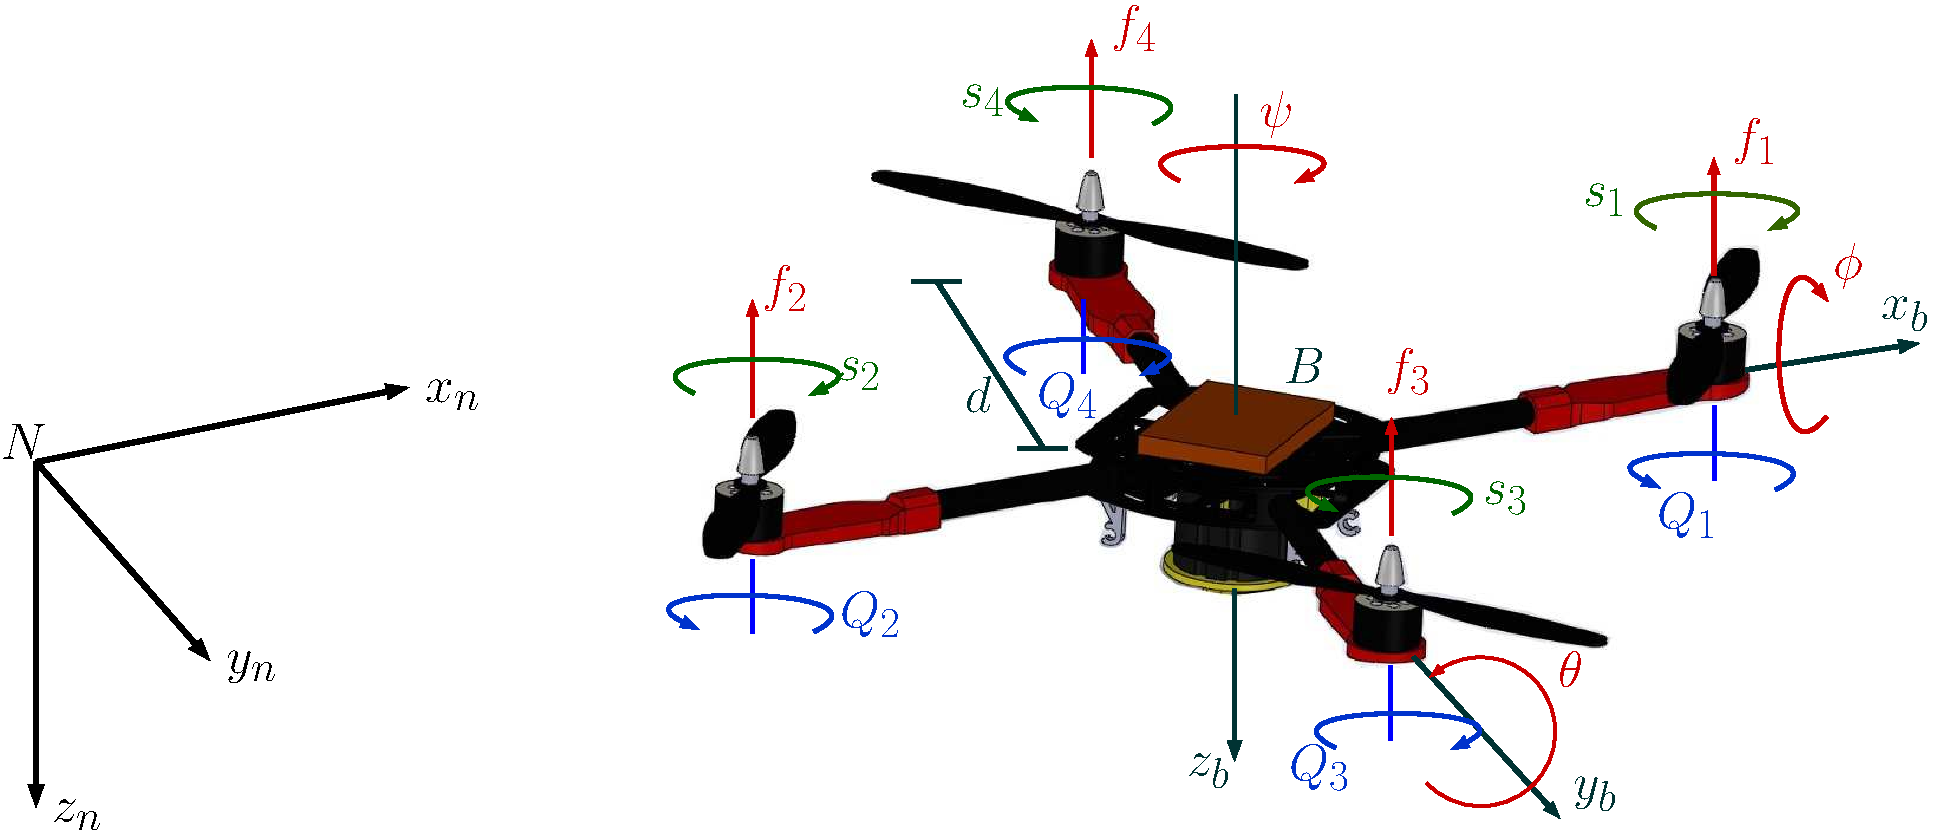
\includegraphics[width =0.9\textwidth]{figures/quadoperation.pdf}
     \caption{Scheme of the quadrotor configuration: inertial reference frame $N(x_n,y_n,z_n)$, the reference body fixed frame $B(x_b,y_b,z_b)$, the $f_i$ forces on each motor, angular velocity of the motors $s_{i}$ and the reaction torques $Q_i$.}
     \label{fig:fourrotor}
   \end{figure}

 Each rotor produces a force $f_i$ parallel to its rotation axe, as well as a drag torque $Q_i$, opposite to the direction of rotation. The total force or total thrust acting on the helicopter (parallel to the $z_b$ axis) is the addition of the four forces generated by each rotor $(F_T=f_1+f_2+f_3+f_4)$. The combination of these forces and the drag torques allow the angular motions over the main axes of the helicopter. Consequently, three movements for the position are produced, see \fig{fig:angmotion}.
 \begin{itemize}
   \item \textbf{Roll} ($\phi$): It is produced by the difference $f_3-f_4$. To obtain this, the velocity of the right motor $m_3$ is increased/reduced, while the velocity of the motor $m_4$ is equally decreased/increased. This difference of forces produces a torque $\Gamma_\phi$ around the axis $x_b$.
   \item \textbf{Pitch} ($\theta$): It is produced by the difference $f_1-f_2$. It is obtained similarly using the front and rear motors $m_1$ and $m_3$. This difference of forces produces a torque $\Gamma_\theta$ around the axis $y_b$.
   \item \textbf{Yaw} ($\psi$): It is the combination of all the reactive torques, $Q_1+Q_2-Q_3-Q_4$. It is obtained by decreasing/increasing the speed of the front and rear motors while decreasing/increasing the speed of the lateral motors. In other words, if a difference of speed between the motors turning in the opposite direction is produced, the reactive torques produce a torque $\Gamma_\psi$ around the axis $z_n$.
   \item \textbf{Vertical displacement on the $x_n$ axis}: To go forward or back, the rotational speed of motor $m_2$ must be decreased/increased, while decreasing/increasing the rotational speed of the motor $m_1$.
   \item \textbf{Lateral displacement on the $y_n$ axis}: To go to the right or left, the rotational speed of the lateral motors $m_4$ and $m_3$ must be decreased/increased.
   \item \textbf{Displacement on the $z_n$ axis}: To go up or down, the torque of all the rotors $m_i$ must be decreased/increased. In the absence of disturbances, the aerial system can perform a hover at a certain height by having a zero translation speed. Then, the total thrust $F_T$ must balance the weight $mg$ of the aerial system by pointing its direction in the axe $z_b$.
 \end{itemize}

 The first three movements are considered for the body fixed frame, and the last three for the inertial reference frame.
 \begin{figure}[h!]
     \centering
     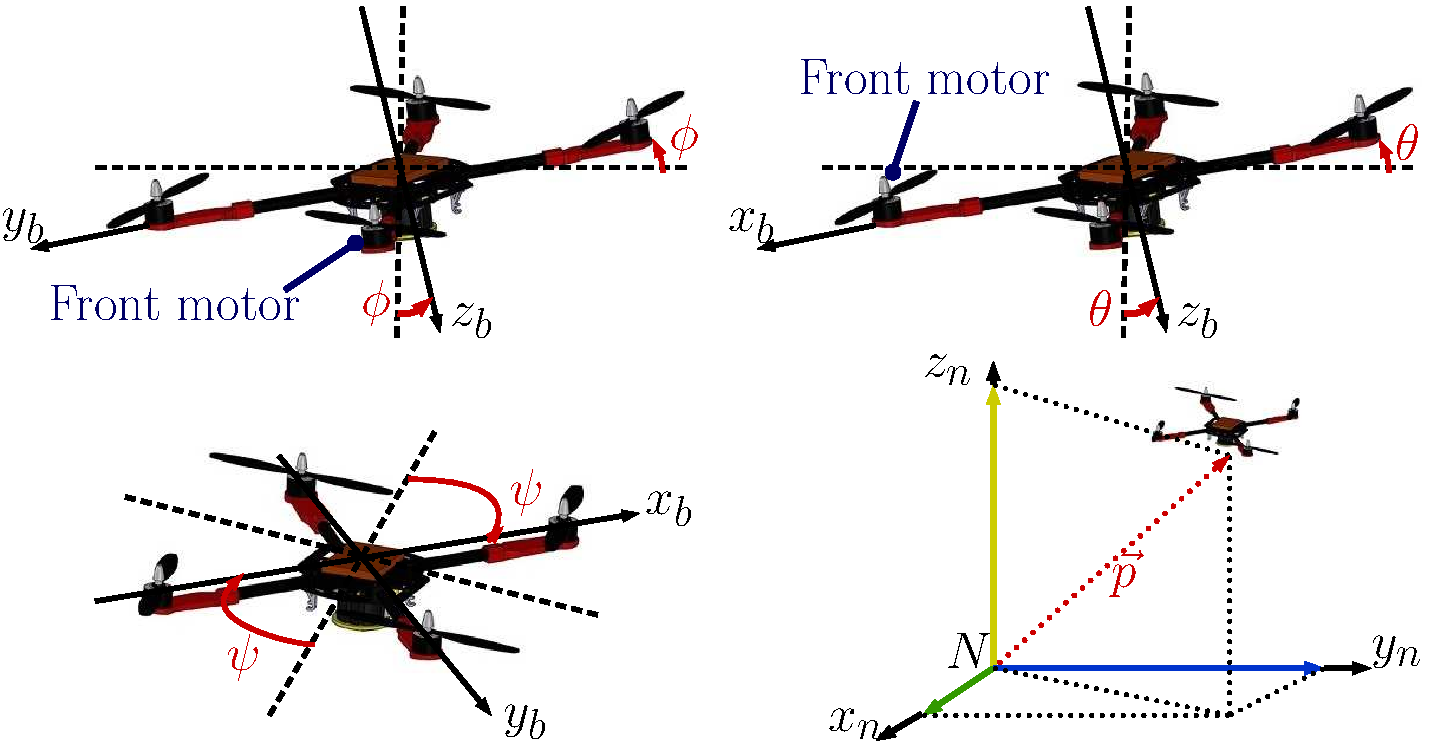
\includegraphics[width =0.8\textwidth]{figures/rollpitchyaw2.pdf}
     \caption{Roll ($\phi$), pitch ($\theta$), yaw ($\psi$) and space displacement}
     \label{fig:angmotion}
   \end{figure}

 From the description of the different angular movements and the vertical and horizontal displacements, it is visible that the position of the system depends on its attitude. In this way, the displacement of the quadcopter can be controlled from the attitude control.


 \section{Position representation}

 Robot tasks are often defined by the use of Cartesian coordinates. Let consider the scheme in \fig{fig:frame_pos}. It is possible to specify the coordinates of the point $p$ with respect to either frame $o_0x_0y_0$ or frame $o_1x_1y_1$.

 Geometrically, a point corresponds to a specific location in space, and a vector specifies a direction and a magnitude. Vectors can be used, for example, to represent displacements or forces. Therefore, while the point $p$ is not equivalent to the vector $\upsilon_1$, the displacement from the origin $o_0$ to the point $p$ is given by the vector $\upsilon_1$. Under this convention, it is clear that points and vectors are not equivalent, since points refer to specific locations in space, but a vector can be moved to any location in space. Then, two vectors are said to be equal if they have the same direction and the same magnitude.

 When assigning coordinates to vectors, the same notational convention is used as when assigning coordinates to points. Thus, $\upsilon_1$ and $\upsilon_2$ are geometric entities that are invariant with respect to the choice of coordinate systems, but the representation by coordinates of these vectors depend directly on the choice of reference coordinate frame.\\
 Using this convention, an expression of the form $\upsilon_1^1+\upsilon_2^2$ where $\upsilon_1^1$ and $\upsilon_2^2$ are as in \fig{fig:frame_pos}, is not defined since the frames $o_0x_0y_0$ and $o_1x_1y_1$ are not parallel. Thus, a clear need appears, not only for a representation system that allows points to be expressed with respect to various coordinate systems, but also for a mechanism that allows to transform the coordinates of points that are expressed in one coordinate system into the appropriate coordinates with respect to some other coordinate frame.
 \begin{figure}[h]
     \centering
     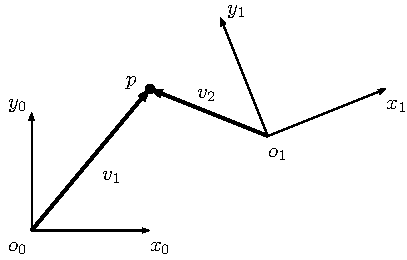
\includegraphics[width =0.5\textwidth]{figures/frame_pos.pdf}
     \caption{Two coordinate frames, a point $p$, and two vectors $\upsilon_1$ and $\upsilon_2$, (\cite{Spong:2004}).}
     \label{fig:frame_pos}
   \end{figure}

 \section{Rigid body attitude representation}

 Consider two orthogonal right-handed coordinate frames: the body coordinate frame, $B(x_b,y_b,z_b)$ located at the center of mass of the rigid body and the inertial coordinate frame, $N(x_n,y_n,z_n)$, located at some point in the space (for instance, the earth NED frame). This coordinate system is showed in \fig{fig:inertial_fixed}. In general, the origin of $B$ is chosen to coincide with the gravity center (CG) of the body.

 The body attitude in the space can be represented in many ways, each one with their advantages and disadvantages, depending mainly on the application.
 \begin{figure}[H]
     \centering
     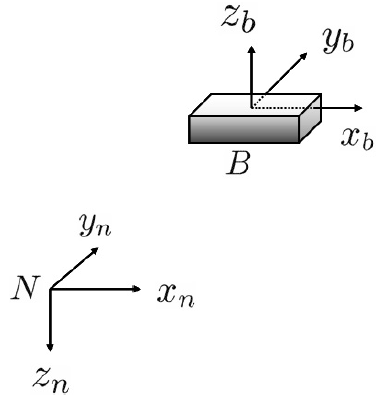
\includegraphics[width =0.28\textwidth]{figures/inertial_fixed.png}
     \caption{Inertial and mobile frame of a rigid body.}
     \label{fig:inertial_fixed}
   \end{figure}

 \begin{definition}
 The movement of a rigid body with reference frame B relative to a rigid body or reference frame N is called a simple rotation of B in N, if there is a line L, called rotation axis, where the orientation relative to B and N keeps the same between the start and the end of the movement.
 \end{definition}
 \begin{theorem}
    (Rotation Euler Theorem). Every relative change in orientation between two rigid bodies with the two coordinate systems B and N can be produced by one simple rotation of B over N.
 \end{theorem}
 Let $\vec{b}$ and $\vec{r}$ be the coordinates of a vector $\vec{X}$ in $B$ and $N$ respectively. Vector $\vec{b}$ can be written in terms of vector $\vec{r}$.

 Let $\vec{e} = [e_1\,\, e_2\,\, e_3]$ be a unit vector collinear to the rotation axis $L$ around which $B$ is rotated by an angle $\beta$. Consequently, $\vec{b}$ is obtained by
 \begin{equation}\label{eq:b}
 \vec{b} = \cos \beta \vec{r} + (1 - \cos \beta)\vec{e}\ \vec{e}\ ^T\vec{r} - \sin\beta\vec{e} \times \vec{r}
 \end{equation}
 In fact, the coordinates $\vec{b}$ and $\vec{r}$ are linked by means of the following linear transformation:
 \begin{equation}
 \vec{b} = C\vec{r}
 \end{equation}
 Matrix $C$ can be token as an operator which takes a fixed vector $\vec{r}$ expressed in $N$ and is expressed in $B$. From (\ref{eq:b})
 \begin{equation}
 C = \cos\beta I_3 + (1 - \cos\beta)\vec{e}\ \vec{e}\ ^T - \sin\beta[\vec{e}\ ^\times]
 \end{equation} where $I_3$ represents the identity matrix of dimension three and $[\xi^\times]$ represents the skew-symmetric matrix, given by:
 \begin{equation}\label{skew}
   [\xi^\times]=\left(\begin{array}{c}
                  \xi_1 \\
                  \xi_2 \\
                  \xi_3
                \end{array}\right)^\times=\left(
                                                  \begin{array}{ccc}
                                                    0 & \xi_3 & \-\xi_2 \\
                                                    -\xi_3 & 0 & \xi_1 \\
                                                    \xi_2 & -\xi_1 & 0 \\
                                                  \end{array}\right)
 \end{equation}
 Matrix $C \in \mathbb{R}^{3\times3}$ identifies the orientation of the moving frame $B$ with respect to the inertial frame $N$ and it allows the coordinate transformation of a vector system into another one. This matrix is known as the direction cosine matrix (DCM), rotation matrix or attitude matrix.

 \subsubsection{Rotation matrix}

 Rotation matrix $C$ belongs to the subspace of orthogonal matrices of dimension three, called special orthogonal group, denoted by $S0(3)$, and defined by
 \begin{equation}\label{so3}
   S0(3)={C|C\in \mathbb{R}^{3\times3},C^TC=I_3,\det(C)=1}
 \end{equation}
 In a rotation matrix $C$, each element $c_{ij}$ is a direct cosine, given by:
 \begin{equation}\label{C}
   C=\left(
       \begin{array}{ccc}
         c_{11} & c_{12} & c_{13} \\
         c_{21} & c_{22} & c_{23} \\
         c_{31} & c_{32} & c_{33} \\
       \end{array}\right)
 \end{equation} where
 \begin{equation}\label{cij}
   c_1=\left(
         \begin{array}{c}
           c_{11} \\
           c_{21} \\
           c_{31} \\
         \end{array}\right)\ \ c_1=\left(
         \begin{array}{c}
           c_{12} \\
           c_{22} \\
           c_{32} \\
         \end{array}\right)\ \ c_1=\left(
         \begin{array}{c}
           c_{13} \\
           c_{23} \\
           c_{33} \\
         \end{array}\right)
 \end{equation}
 Consequently,
 \begin{equation}\label{C2}
   C=\left(
       \begin{array}{ccc}
         c_1 & c_2 & c_3 \\ \end{array}\right)
 \end{equation} where
 \begin{equation}
   c_i^Tc_i=1\ \ \textrm{and}\ \ c_i^Tc_j=0\ \ \forall i\neq j
 \end{equation}

 \subsubsection{Rotational velocity}

 Suppose that a rotation matrix $C$ is time varying, so that $C=C(t)\ \in\ S0(3)$ for every $t\ \in\ \mathbb{R}$. Assuming that $C(t)$ is continuously differentiable as a function of $t$. An argument identical to the one in the previous section shows that the time derivative $\dot{C}(t)$ of $C(t)$ is given by
 \begin{equation}
   \dot{C}(t)=[\vec{\omega}\ ^\times]C(t)
 \end{equation} where $\vec{\omega}$ is the angular velocity of the rotating frame with respect to the fixed frame at time $t$.

 \subsubsection{Euler angles and Roll, Pitch and Yaw angles}
 \begin{figure}[H]
     \centering
     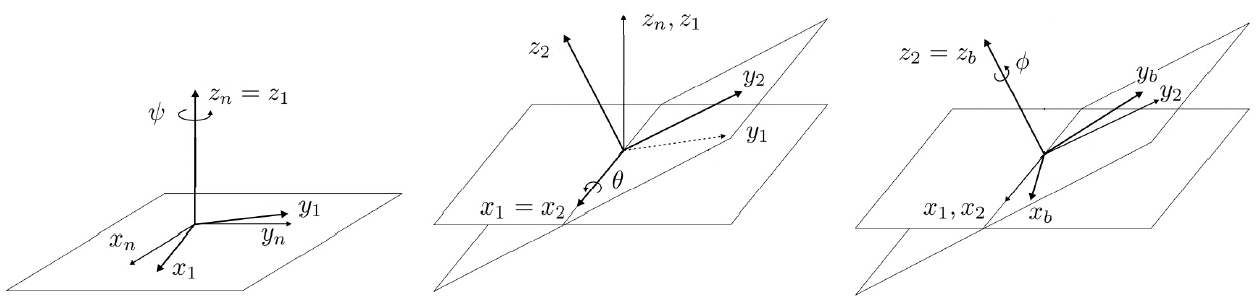
\includegraphics[width =\textwidth]{figures/euler.png}
     \caption{Euler angles.}
     \label{fig:euler_an}
   \end{figure}

 A common method of specifying a rotation matrix in terms of three independent quantities is to use the so-called Euler Angles $(\psi,\theta,\varphi)$. Consider again the fixed coordinate frame $N(x_n,y_n,z_n)$ and the rotated frame $(x_b,y_b,z_b)$, shown in \fig{fig:euler_an}.

 It is possible to specify the orientation of the frame $(x_1,y_1,z_1)$ relative to the frame $N(x_n,y_n,z_n)$ by the three angles, and it can be obtained by three successive rotations as follows: first rotate about z-axis by the angle $\phi$, next, rotate about the current y-axis by the angle $\theta$. Finally, rotate about the current z-axis by the angle $\psi$.
 In terms of the basic rotation matrices the resulting rotational transformation $C_1^0$ can be generated as the product
 \begin{equation}\label{euler}
 \begin{split}
 C_1^0=C_{z,\phi},C_{y,\theta},C_{z,\psi} &= \left[\begin{array}{ccc}
                                                      c_\phi & -s_\phi & 0 \\
                                                      s_\phi & c_\psi & 0 \\
                                                      0 & 0 & 1 \end{array}\right]\left[\begin{array}{ccc}
                                                                                          c_\theta & 0 & s_\theta \\
                                                                                          0 & 1 & 0 \\
                                                                                          -s_\theta & 0 & c_\theta \end{array}\right]\left[\begin{array}{ccc}
                                                                                                                    c_\psi & -s_\psi & 0 \\
                                                                                                                    s_\psi & c_\psi & 0 \\
                                                                                                                     0& 0 & 1
                                                                                                                  \end{array}
                                                                                          \right]\\
                                                      &=\left[\begin{array}{ccc}
                                                        c_\phi c_\theta c_\psi-s_\phi s_\psi & -c_\phi c_\theta s_\psi-s_\phi c_\psi & c_\phi s_\theta \\
                                                        s_\phi c_\theta c_\psi+c_\phi s_\psi & -s_\phi c_\theta s_\psi+c_\phi c_\psi & s_\phi s_\theta \\
                                                        -s_\theta c_\psi & s_\theta s_\psi & c_\theta                     \end{array}\right]
 \end{split}
 \end{equation}

 A rotation matrix $C$ can also be described as a product of successive rotations about the principal coordinate axes $x_n$, $y_n$ and $z_n$ taken in a specific order. These rotations define the roll, pitch and yaw angles. The order of rotations is specified as $z-y-x$, in other words, first a yaw about $z_n$ by an angle $\phi$, then pitch about the $y_n$ by an angle $\theta$, and finally roll about the $x_n$ by an angle $\psi$. Since the successive rotations are relative to the fixed frame, the resulting transformation matrix is given by
 \begin{equation}\label{euler}
 \begin{split}
   C_1^0=C_{z,\phi}C_{y,\theta}C_{x,\psi}&=\left[\begin{array}{ccc}
                                                   c_\phi & -s_\phi & 0 \\
                                                   s_\phi & c_\phi & 0 \\
                                                   0 & 0 & 1
                                                 \end{array}
   \right]\left[\begin{array}{ccc}
                  c_\theta & 0 & s_\theta \\
                  0 & 1 & 0 \\
                  -s_\theta & 0 & c_\theta
                \end{array}\right]\left[\begin{array}{ccc}
                                          1 & 0 & 0 \\
                                          0 & c_\psi & -s_\psi \\
                                          0 & s_\psi & c_\psi
                                        \end{array}\right] \\
                                        &=\left[\begin{array}{ccc}
                                                c_\phi c_\theta & -s_\phi c_\psi+c_\phi s_\theta s_\psi & s_\phi s_\psi+c_\phi s_\theta c_\psi \\
                                                s_\phi c_\theta & c_\phi c_\psi+s_\phi s_\theta s_\psi & -c_\phi s_\psi+s_\phi s_\theta c_\psi \\
                                                -s_\theta & c_\theta s_\psi & c_\theta c_\psi
                                              \end{array}\right]
 \end{split}
 \end{equation}

 Now, let $\vec{\omega}=[\begin{array}{ccc}\omega_x & \omega_y & \omega_z\end{array}]$ be the angular velocity of the body in the reference frame $B$ with respect to the reference frame $N$. Then, the kinematic equation is given by \cite{Fossen:1994}:
 \begin{equation}\label{vitesse}
   \left(\begin{array}{c}
           \dot{\phi} \\
           \dot{\theta} \\
           \dot{\psi}\end{array}\right)=\left(\begin{array}{ccc}
                                                1 & \tan\theta\sin\phi & \tan\theta\sin\phi \\
                                                0 & \cos\phi & -\sin\phi \\
                                                0 & \frac{\sin\phi}{\cos\theta} & \frac{\cos\phi}{\cos\theta}
                                              \end{array}\right)\left(\begin{array}{c}
                                                                        \omega_x \\
                                                                        \omega_y \\
                                                                        \omega_z
                                                                      \end{array}
                                              \right)
 \end{equation}

 \subsubsection{Quaternions}

 The drawbacks of the angle/axis representation can be overcome by a different four-parameter representation; namely, the unit \emph{quaternion} or Euler parameters, defined by:
 \begin{equation}\label{defquaternion}
         q:=\left(%
 \begin{array}{c}
   \cos \frac{\beta}{2} \\
   \vec{e} \sin \frac{\beta}{2}  \\
 \end{array}%
 \right)=\left(\begin{array}{c}
   q_0 \\
   q_v  \\
 \end{array}\right)   \in \mathbb H
 \end{equation} where
 \begin{equation}\label{H}
   \mathbb H={q|q_0^2+\vec{q}\ ^T\vec{q}=1, \ q=\left(\begin{array}{c}
   q_0 \\
   \vec{q}  \\
 \end{array}\right), \ q_0\in\mathbb{R}, \ \vec{q}\in\mathbb{R}^3}
 \end{equation} where $\vec{q}=(q_1\ \ q_2 \ \ q_3)^T \in \mathbb R^3 $ and $q_0 \in \mathbb R$ are known as the vector and scalar parts of the quaternion respectively. The identity quaternion and the conjugated quaternion are given by:
 \begin{equation}\label{qid}
   q_{id}=[1 \ \ 0^T]\ ^T \ \ \bar{q}=[q_0 \ \ -\vec{q}\ ^T]\ ^T
 \end{equation}
 Since the quaternion is unitary, $q^{-1}=\bar{q}$.
 The product of two quaternions $q_1=[q_{1_{0}} \ \ \vec{q_1}^T]^T$ and $q_2=[q_{2_{0}} \ \ \vec{q_2}^T]^T$ is defined by:
 \begin{equation}\label{multiq}
   q_1\otimes q_2=\left(\begin{array}{cc}
                          q_{1_{0}} & -\vec{q}_1\ ^T \\
                          \vec{q}_1 & I_3q_{1_{0}}+[\vec{q}\ ^\times]
                        \end{array}\right)\left(\begin{array}{c}
                                                  q_{2_{0}} \\
                                                  \vec{q}_2 \end{array}\right)
 \end{equation}

 Now, let $b_q$ and $r_q$ be the quaternions associated to vectors $\vec{b}$ and $\vec{r}$, defined by:
 \begin{equation}
   b_q=[0 \ \ \vec{b}\ ^T]\ ^T \ \ r_q=[0 \ \ \vec{r}\ ^T]\ ^T
 \end{equation}
 These two quaternions are linked by the next relation:
 \begin{equation}
   b_q=q\otimes r_q \otimes q^{-1}=q \otimes r_q \otimes \bar{q}
 \end{equation}

 Rotation matrix $C$ can be expressed in terms of quaternions by:
 \begin{equation}\label{rotq}
   C=C(q)=(q_0^2-\vec{q}\ ^T\vec{q})I_3+2(\vec{q}\ \vec{q}\ ^T-q_0[\vec{q}\ ^\times])
 \end{equation} from where
 \begin{equation}\label{Cq}
   C(q)=\left(\begin{array}{ccc}
                2(q_0^2+q_1^2)-1 & 2(q_1q_2+q_0q_3) & 2(q_1q_3-q_0q_2) \\
                2(q_1q_2-q_0q_3) & 2(q_0^2+q_2^2)-1 & 2(q_0q_1+q_2q_3) \\
                2(q_0q_2+q_1q_3) & 2(q_2q_3-q_0q_1) & 2(q_0^2+q_3^2)-1 \end{array}\right)
 \end{equation}

 The relation between the vectors $\vec{b}$ and $\vec{r}$ is:
 \begin{equation}
   \vec{b}=C(q)\vec{r}
 \end{equation}
 Denoting by $w=(\omega_1\ \ \omega_2\ \ \omega_3)^T$ the angular velocity vector of the body coordinate frame, $B$ relative to the inertial  coordinate frame $N$ expressed in $B$, the kinematics equation is given by
 \begin{equation}\label{eqkinematic}
 \left(%
 \begin{array}{c}
   \dot{q}_0 \\
   \dot{\vec{q}} \\
 \end{array}%
 \right) =  \frac{1}{2}\left(%
 \begin{array}{c}
   -\dot{q}^T \\
   I_3q_0 + [\vec{q}^\times] \\
 \end{array}%
 \right) w=\frac{1}{2}\Xi(q)w
 \end{equation}

 \subsubsection{Rigid motions}

 \begin{definition}
   A rigid motion is an ordered pair (d,C) where $d\ \in\ \mathbb{R}^3$ and $C\ \in\ SO(3)$. The group of all rigid motions is known as the \textbf{Special Euclidean Group} and is denoted by $SO(3)$. It is denoted that $SO(3)=\mathbb{R}^3\times SO(3)$.
 \end{definition}

 A rigid motion is a pure translation together with a pure rotation.

 \subsubsection{Homogeneous transformations}

 The combination of position and orientation representations allows the formulation of homogeneous transformations, used in the modeling of arm manipulators. Then, the transformation matrices with the form:
 \begin{equation}\label{eq:homo}
   H=\left[\begin{array}{cc}
             C & d \\
             0 & 1 \end{array}\right]
 \end{equation} are called \textbf{homogeneous transformations}. Then, a homogeneous transformation is a representation of a rigid motion where the system $S0(3)$ is used interchangeably to represent the set of rigid motions and the set of all $4\times4$ matrices given in (\ref{eq:homo}).

 A set of basic homogeneous transformations generating $S0(3)$ is given by
 \begin{equation}\label{transx}
   Trans_{x,a}=\left[\begin{array}{cccc}
                       1 & 0 & 0 & a \\
                       0 & 1 & 0 & 0 \\
                       0 & 0 & 1 & 0 \\
                       0 & 0 & 0 & 1 \end{array}\right];\ \ Rot_{x,a}\left[\begin{array}{cccc}
                                                                            1 & 0 & 0 & 0 \\
                                                                            0 & c_a & -s_a & 0 \\
                                                                            0 & s_a & c_a & 0 \\
                                                                            0 & 0 & 0 & 1 \end{array}\right]
 \end{equation}
 \begin{equation}\label{transx}
   Trans_{y,b}=\left[\begin{array}{cccc}
                       1 & 0 & 0 & 0 \\
                       0 & 1 & 0 & b \\
                       0 & 0 & 1 & 0 \\
                       0 & 0 & 0 & 1 \end{array}\right];\ \ Rot_{y,b}\left[\begin{array}{cccc}
                                                                            c_\beta & 0 & s_\beta & 0 \\
                                                                            0 & 1 & 0 & 0 \\
                                                                            -s_\beta & 0 & c_\beta & 0 \\
                                                                            0 & 0 & 0 & 1 \end{array}\right]
 \end{equation}
 \begin{equation}\label{transx}
   Trans_{z,c}=\left[\begin{array}{cccc}
                       1 & 0 & 0 & 0 \\
                       0 & 1 & 0 & 0 \\
                       0 & 0 & 1 & c \\
                       0 & 0 & 0 & 1 \end{array}\right];\ \ Rot_{x,a}\left[\begin{array}{cccc}
                                                                            c_\gamma & -s_\gamma & 0 & 0 \\
                                                                            s_\gamma & c_\gamma & 0 & 0 \\
                                                                            0 & 0 & 1 & 0 \\
                                                                            0 & 0 & 0 & 1 \end{array}\right]
 \end{equation} for translation and rotation about the $x,y,z$ axis respectively.\\
 The most general homogeneous transformation that is considered is given by
 \begin{equation}\label{homogen}
   H_1^0=\left[\begin{array}{cccc}
                 n_x & s_x & a_x & d_x \\
                 n_y & s_y & a_y & d_y \\
                 n_z & s_z & a_z & d_z \\
                 0 & 0 & 0 & 1 \end{array}\right]=\left[\begin{array}{cccc}
                                                          n & s & a & d \\
                                                          0 & 0 & 0 & 1 \end{array}\right]
 \end{equation}
 In the above equation $n=(n_x,n_y,n_z)^T$ is a vector representing the direction of $X_1$ in the $o_0x_0y_0$ system, $s=(s_x,s_y,s_z)^T$ represents the direction of $y_1$, and $a=(a_x,a_y,a_z)$ represents the direction of $z_1$. $d=(d_x,d_y,d_z)^T$ represents the vector from the origin $o_0$ to the origin $o_1$ expressed in the frame $o_0x_0y_0z_0$.

 \subsubsection{Attitude error}

 Two orientations of a rigid body are considered, described by rotation matrices $C_1$ and $C_2$ respectively. Then, the relative attitude between these two orientations is computed by:
 \begin{equation}\label{Cr}
   C_r=C_1^{-1}C_2
 \end{equation}
 In fact, $C_r$ represents an operator of orientation which rotates $C_2$ about $C_1$. From here, the relative orientation is used in the estimation and in the orientation control as \emph{attitude error}. With this, $C_d=C_1$ is the desired attitude of a rigid body and $C=C_2$ is the real attitude of the body.
 Consequently, the attitude error is computed by:
 \begin{equation}\label{Ce}
   C_e=C_d^{-1}C
 \end{equation}
 If the attitude error is zero, then, $C_e=I_3$.
 When the unitary quaternion is used to represent the attitude of the body, the relative orientation between $q_1$ and $q_2$ is expressed by:
 \begin{equation}\label{qr}
   q_r=q_1^{-1}\otimes q_2=\left(\begin{array}{cc}
                                  q_{1_{0}} & \vec{q}_1\ ^T \\
                                  -\vec{q}_1 & I_3q_{1_{0}}-[\vec{q}\ ^\times]\end{array}
   \right)\left(\begin{array}{c}
                  q_{2_0} \\
                  \vec{q}_2 \end{array}\right)=\bar{q}_1\otimes q_2
 \end{equation}
 The geodesic metric is given by the next expression:
 \begin{equation}\label{betar}
   \beta_r=2|\arccos(q_{r_{0}})|
 \end{equation}
 This metric represents the smallest angle of rotation between attitude $q_1$ and the attitude $q_2$. The Euclidean distance between the two unitary quaternions gives an approximation of the geodesic metric:
 \begin{equation}\label{geodesic}
   \frac{2}{\pi}\beta_r\leq2\parallel q_1-q_2\parallel_2\leq\beta_r
 \end{equation}
 Also, when $\beta_r$ is enough small, it is possible to do the next approximation:
 \begin{equation}\label{approx}
   \beta_r\approx2\parallel q_1-q_2\parallel_2
 \end{equation}

 For the case of the attitude control law, if $q_d=q_1$ is the desired attitude of the body and $q=q_2$ is the real attitude of the body, the attitude error is given by:
 \begin{equation}\label{qerr}
   q_e=q_d^{-1}\otimes q=\bar{q}_d\otimes q
 \end{equation}
 When the attitude error is zero, the error quaternion has two possible values:
 \begin{equation}\label{qe1}
   q_e=[\pm1 \ \ 0]^T
 \end{equation}
 This is due to the non bijection quaternion with the group $SO(3)$.

% \subsection{Notation and axis system}
% \subsection{Dinamic model of a mini-UAV}

 \section{Conclusions}

%
\clearemptydoublepage
% % \chapter{State of the art of aerial manipulation}
<<<<<<< current
%!TEX root = ../thesis.tex
%*******************************************************************************
%****************************** Third Chapter **********************************
%*******************************************************************************
\chapter{Pose estimation using a single camera}%Lateral and height

% **************************** Define Graphics   Path **************************
\ifpdf
    \graphicspath{{Chapter3/Figs/Raster/}{Chapter3/Figs/PDF/}{Chapter3/Figs/}}
\else
    \graphicspath{{Chapter3/Figs/Vector/}{Chapter3/Figs/}}
\fi


UAV autonomous navigation into corridors or tunnels is a hard task due mainly to the localization problem. GPS measurements are usually dropped noised or unavailable. Cameras become a popular sensors for pose estimation even if sometimes is hard to compute on-board the algorithm. This chapter is centered on the estimation of the relative position of the vehicle through a single image in real-time execution. This information is useful since it serves to make an indoor navigation (in a corridor). The algorithm designed is intended to use the minimum of resources of the computer. Although this first stage focuses on using tools such as matlab, the algorithms can be easily implemented in an embedded system. So the program can be resume as follow: firstly the virtual image is obtained. Then the edges of the image are extracted.  The rotation %This extracted information are all the lines obtained from the edges of doors, windows, walls, corners, etc.
matrix of the camera is estimated using infinite vanishing points and finite vanishing points. A new sub-classification of lines is made from the finite vanishing point. This subset is done in four quadrants. Using the finite vanishing point and the information of each quadrant, we can obtain the principal line from each corner. The collinearity property is used with pairs of major lines. If there is a collinearity between each pair of lines the system is centered. Otherwise, the result is a percentage of displacement in the \textit{y}-axis, \textit{z}-axis.  The scale is a percentage of displacement where the center of the corridor indicates a zero percentage of displacement. A numerical validation is made in order to verify this algorithm.

\section{Pose estimation algorithm}

 The proposed vision algorithm takes into account the perspective projection, the vanish point identification and the collinearities of the principal lines in the image to estimate the pose of an aerial vehicle. 0.2cm Ideas from \cite{Akinlar2011, boulanger:inria-00461526} and \cite{Lee2009} have inspired our algorithm.  The general scheme of the estimation pose algorithm can be seen in Figure \ref{fig:1_algo}. As can be observed in this figure, once the image is acquired a line
detector algorithm is applied. For making a subset of vertical, horizontal and diagonal lines a histogram is then used. After that, the rotation matrix is acquired and the line classification algorithm is again applied for extracting principal lines in the image. This information is used with the collinearity approach for estimating the pose of the camera. Therefore it is relatively easy compute the \textit{y} and \textit{z}-axis in the image plane.

Figure \ref{fig:VisionAlgoritm} shows the general procedure, and  this  depics too the vanishing point evolution. For obtaining the pose estimation it is necessary to know the camera model, next subsections will introduce this concept and each block in the general scheme algorithm.

\begin{figure*}[h!]
\centering
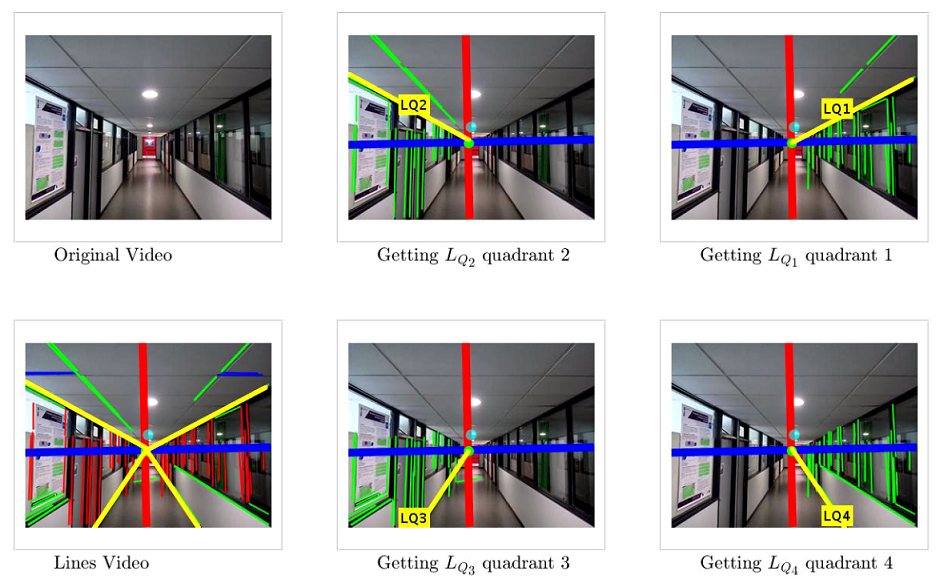
\includegraphics[width=0.85\textwidth]{Chapter03/Images/Algoritme_m.png}
\caption{These images introduce the applied methodology. The scene is a corridor and an image is taken from the video to extract a set of lines that could describe geometrically the environment and the rotation matrix. Four new subsets of lines are made taking into account the vanishing point (quadrant 1, 2, 3 and 4). The information of each quadrant is used to obtain the principal lines (LQ1, LQ2, LQ3, LQ4). }
\label{fig:VisionAlgoritm}
\end{figure*}


\subsection{Vanishing point algorithm}
Perspective projection of parallel lines in world space creates vanishing lines in image space that
intersect in a point called vanishing point. If the parallel lines are parallel to the image plane,
the vanishing lines are also parallel to this plane and the vanishing point is at an infinite
distance from the image center, hence is called infinite vanishing point. Otherwise, it is a finite
vanishing point. For our case the camera calibration is based on the following assumption: the main vanishing lines in the input image correspond to three orthogonal directions in world space as can be seen in Figure \ref{fig:VisionAlgoritm}.

\subsection{Dominant lines detection}
In man-made indoor environments, it is possible to extract line segments, texture, colors and so on.
In this work,  the linear time line segment detector called EDlines \cite{Akinlar2011} is used giving accurate results and with high time process (all the segments for an image $240 \times3 20$ are computed in 3 $ms$). This algorithm no requires parameter tuning and run ups faster than others methods as the Hough transform \cite{HoughMAtlab}.

\subsection{Lines classification}

RANSAC (Random Sample Consensus) has become  a simple and powerful method to %various authors have been developed and introduced RANSAC as
provide a partition of parallel straight lines into clusters by
pruning outliers. \color{blue} The algorithm begins selecting randomly  two lines for generating a VP hypothesis.  These lines  are grouped together in order to optimize the estimated VP and for obtaining a dominant VP.
When a dominant VP is obtained, the process finishes. Nevertheless, several finite vanishing points can be
extracted from the environment with this algorithm. \color{black} \vskip 0.2cm


In the context of indoor navigation, the main orthogonal
directions in environments consist generally in a vertical
one (often associated with an infinite VP) and two horizontal
ones (associated with finite or infinite VP). In this work, the heuristic strategy is taken  to extract a
limited number of reliable VP while enforcing the
orthogonality constraint, in conjunction with RANSAC.  \vskip 0.2cm

For a robust selection of VPs, an histogram is made in order to classify
all the set of lines in a subset of vertical lines  $L_v$, a subset of horizontal lines $L_h$ and a subset
of diagonal lines $L_d$. For clustering lines by RANSAC, the consensus score is quite different
depending on each subset and is computing with (\ref{RansacVP1}). Unlike the finite VP whose coordinates may be determined in
the image plan (lines $L_d$), the infinite VPs are generally represented with a
direction (lines $L_v$, $L_h$). For finite VP, the consensus score is based on a
distance between the candidate straight line and the
intersecting point and represented as (\ref{RansacVP2}). For infinite VP, it is obtained with (\ref{RansacIVP}) using the angular
distance between the direction of the candidate straight line
and the direction representing the infinite VP,  more details see \cite{Elloumi2014}.

\begin{eqnarray}
	score &=&  \sum_{i=0}^{n} \Upsilon(v,l_i)  \label{RansacVP1} \\
  	\Upsilon(v,l_i)  &=&  \left \{\begin{array}{ll}
 	                   1 & d(v,l_i) < \delta\\
 	                   0 &  \text{otherwise}
 	                  \end{array} \right.       \label{RansacVP2} \\
	 \Upsilon(v,l_i) &=&  \left \{\begin{array}{ll}
 	                   1 & Min(\widehat{(\overrightarrow{v},\overrightarrow{l_i})},\widehat{(\overrightarrow{l_i},\overrightarrow{v})}) < \delta\\
 	                   0 & \text{otherwise}
 	                  \end{array} \right.   \label{RansacIVP}
 \end{eqnarray}
where $n$ is the number of dominant lines and $d(v, l_i)$ denotes the
Euclidian distance from the finite VP candidate $v$ to the line $l_i$.
The lines whose distance is below a fixed threshold $\delta$ are
considered as participants. $(\overrightarrow{v},\overrightarrow{l_i})$ describes the angle between the infinite VP direction
from the image center and the line $l_i$ to test in image space. \color{black}

\subsection{Rotation matrix estimation}

It is known that when using the VPs intrinsic and extrinsic camera parameters can be estimated. We consider that the intrinsic parameters are known thus we will focus on compute the others ones, in particularly the Rotation matrix.
The main point $p$ of the camera is set to the center of the image plane. The rotation matrix
$(\vec{u},\vec{v},\vec{w})$ transforms points from real world to the image plane. Its columns are the vectors of the world coordinates frame expressed in the camera space. The directions of the three vanishing points from the optical center of the camera are assumed to be orthogonal. Thus without loss of generality, the following relations hold for the final calibrated.

% \begin{subequations}
% \begin{align}
% 	\label{VectorOrto}
% 	f>0 \\
% 	\vec{u} \cdot \vec{v}= \vec{v}\cdot \vec{w}=\vec{w}\cdot \vec{u}=0\\
%   	\abs{\vec{u}}=\abs{\vec{v}}=\abs{\vec{w}}
% \end{align}
% \end{subequations}

The obtained structured lines  from the corridor image provide enough information to estimate the camera rotation matrix.
Normally, it is supposed that the camera has a vertical position, and  as the corridor is plenty of vertical and horizontal lines, then it is possible to find a finite vanishing point and two infinite vanishing points.


\subsubsection*{A finite vanishing point, two infinite vanishing points}

\begin{figure}[h!]
\centering
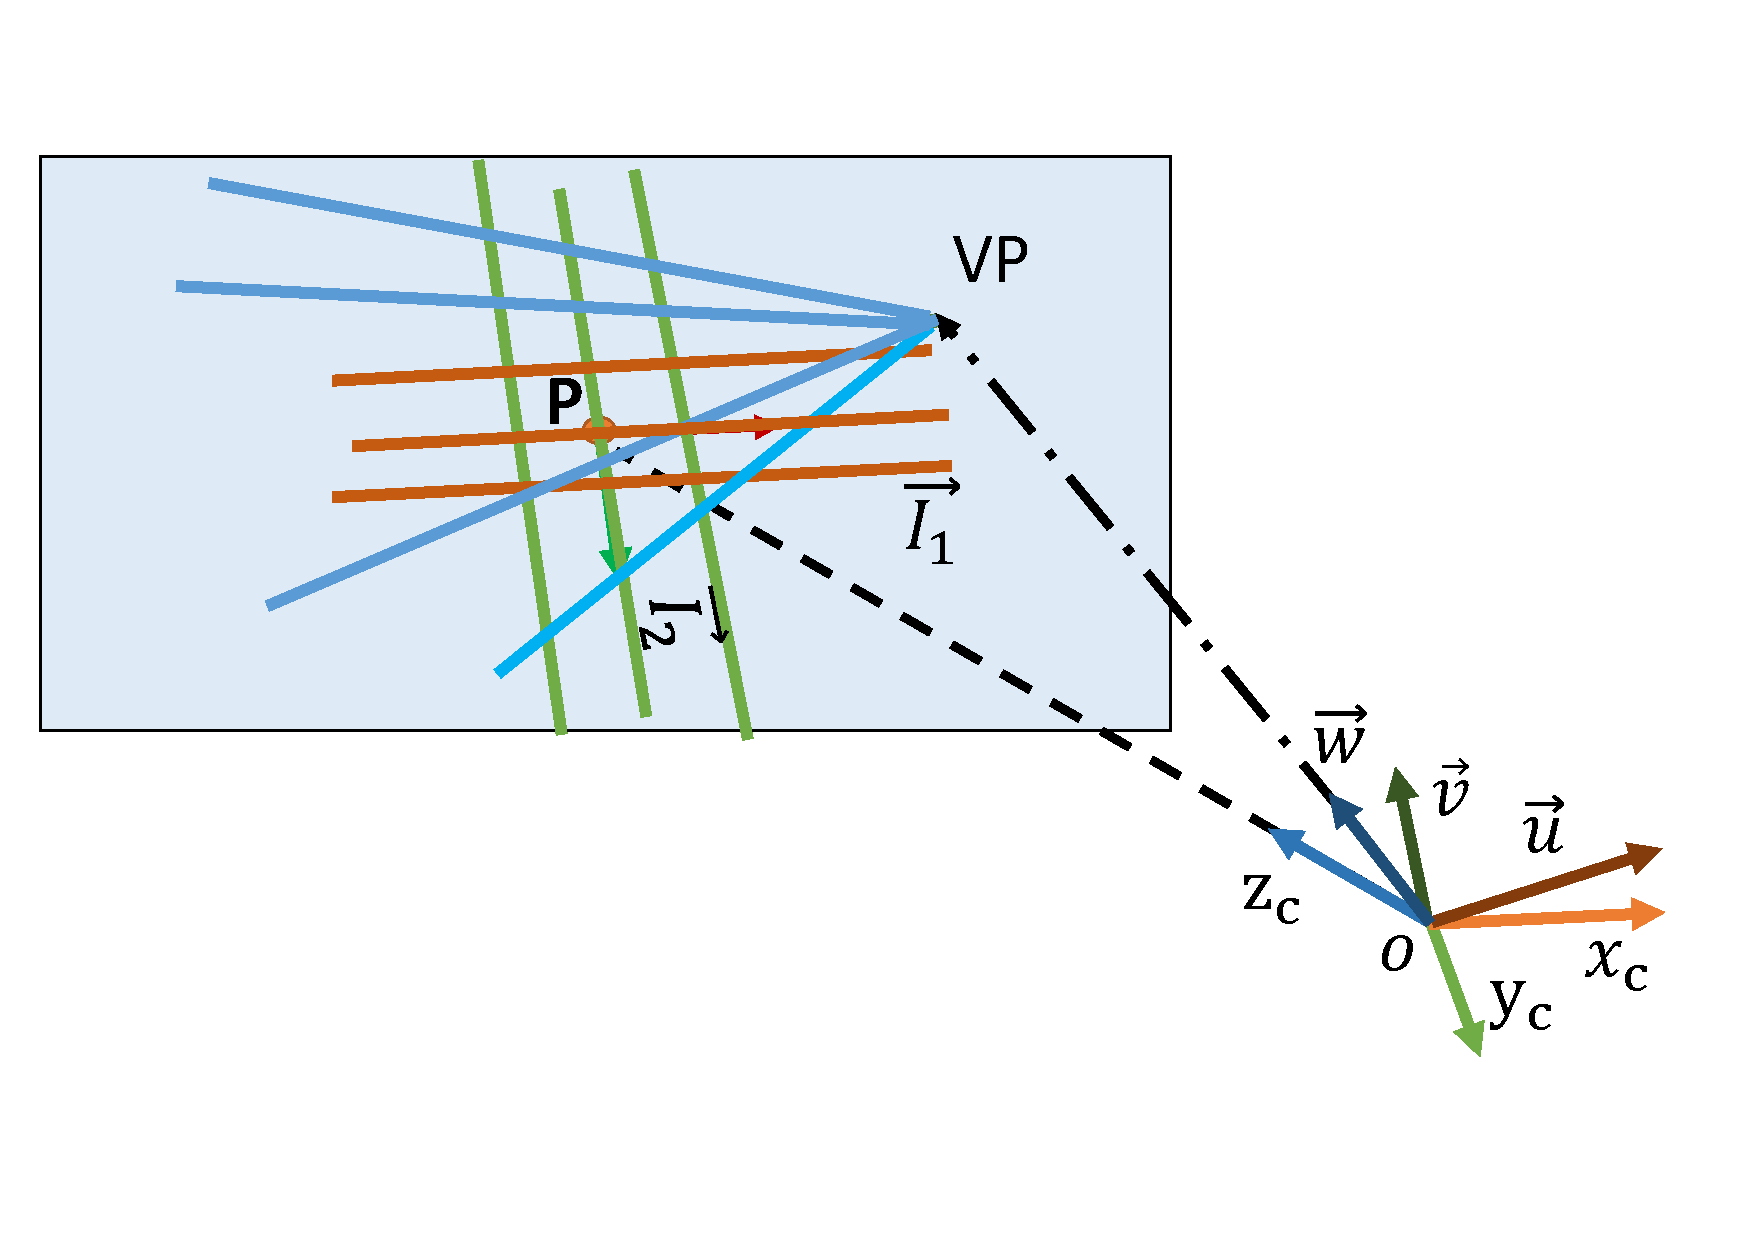
\includegraphics[width=0.8\textwidth]{Chapter03/Images/twoInfiniteVPOneFVPG.pdf}
\caption{Camera calibration with one finite and two infinite vanishing points. $(x_c,y_c,z_c)$ is the camera coordinate frame, $(\vec{u},\vec{v},\vec{w})$ the world coordinate frame, $VP$ the finite vanishing point, $\vec{I_1}$ and $\vec{I_2}$ the infinite vanishing point directions. $P$ is the main point.}
\label{fig:3_unpunto}
\end{figure}

This case occurs when two axes of the world frame are parallel to the image plane.  Fig \ref{fig:3_unpunto}
introduces the terms involved for the camera calibration
using one finite vanishing point $\overrightarrow{OVP} = (vp_{x}, vp_{y},-f )^T$ and
two infinite vanishing points with directions $\vec{I_1} = (I_{1_x}, I_{1_y},0)^T$
and $\vec{I_2} = (I_{2_x}, I_{2_y},0)^T$. \vskip 0.2cm


The vector $\vec{w}'$ defines a non-normalized form of  $\vec{w}$,
and is computed from the finite vanishing point as
\begin{equation}
	\label{oneVanish}
	\vec{w}'= (w_{x}',w_{y}',w_{z}')=\overrightarrow{OVP}=(vp_{x}, vp_{y},-f )
 \end{equation}

The coordinate axis $\vec{u}$, as indicated in Figure \ref{fig:3_unpuntoH}, lies
on the plane defined by the points $O$, $P$ and the direction
$\vec{I_1} = (I_{1_x}, I_{1_y},0)^T$ . Then $\vec{u}'$, the non-normalized version of
$\vec{u}$, can be expressed as $\vec{u}' = (I_{1_x}, I_{1_y},u_{z}')$. The goal is that
$\vec{u}$ and $\vec{w}$ belong into an orthogonal coordinate frame, then
\begin{equation}
	%\label{oneVanish}
	\vec{u}' \cdot  \vec{w}'= I_{1_x}w_{x}'+ I_{1_y}w_{y}'+u_{z}'w_{z}' =0
 \end{equation}
therefore
 \begin{equation}
	\label{PlanoU}
	u_{z}'=\frac{I_{1_x}w_{x}'+ I_{1_y}w_{y}'}{f}
\end{equation}

\begin{figure}[h]
\centering
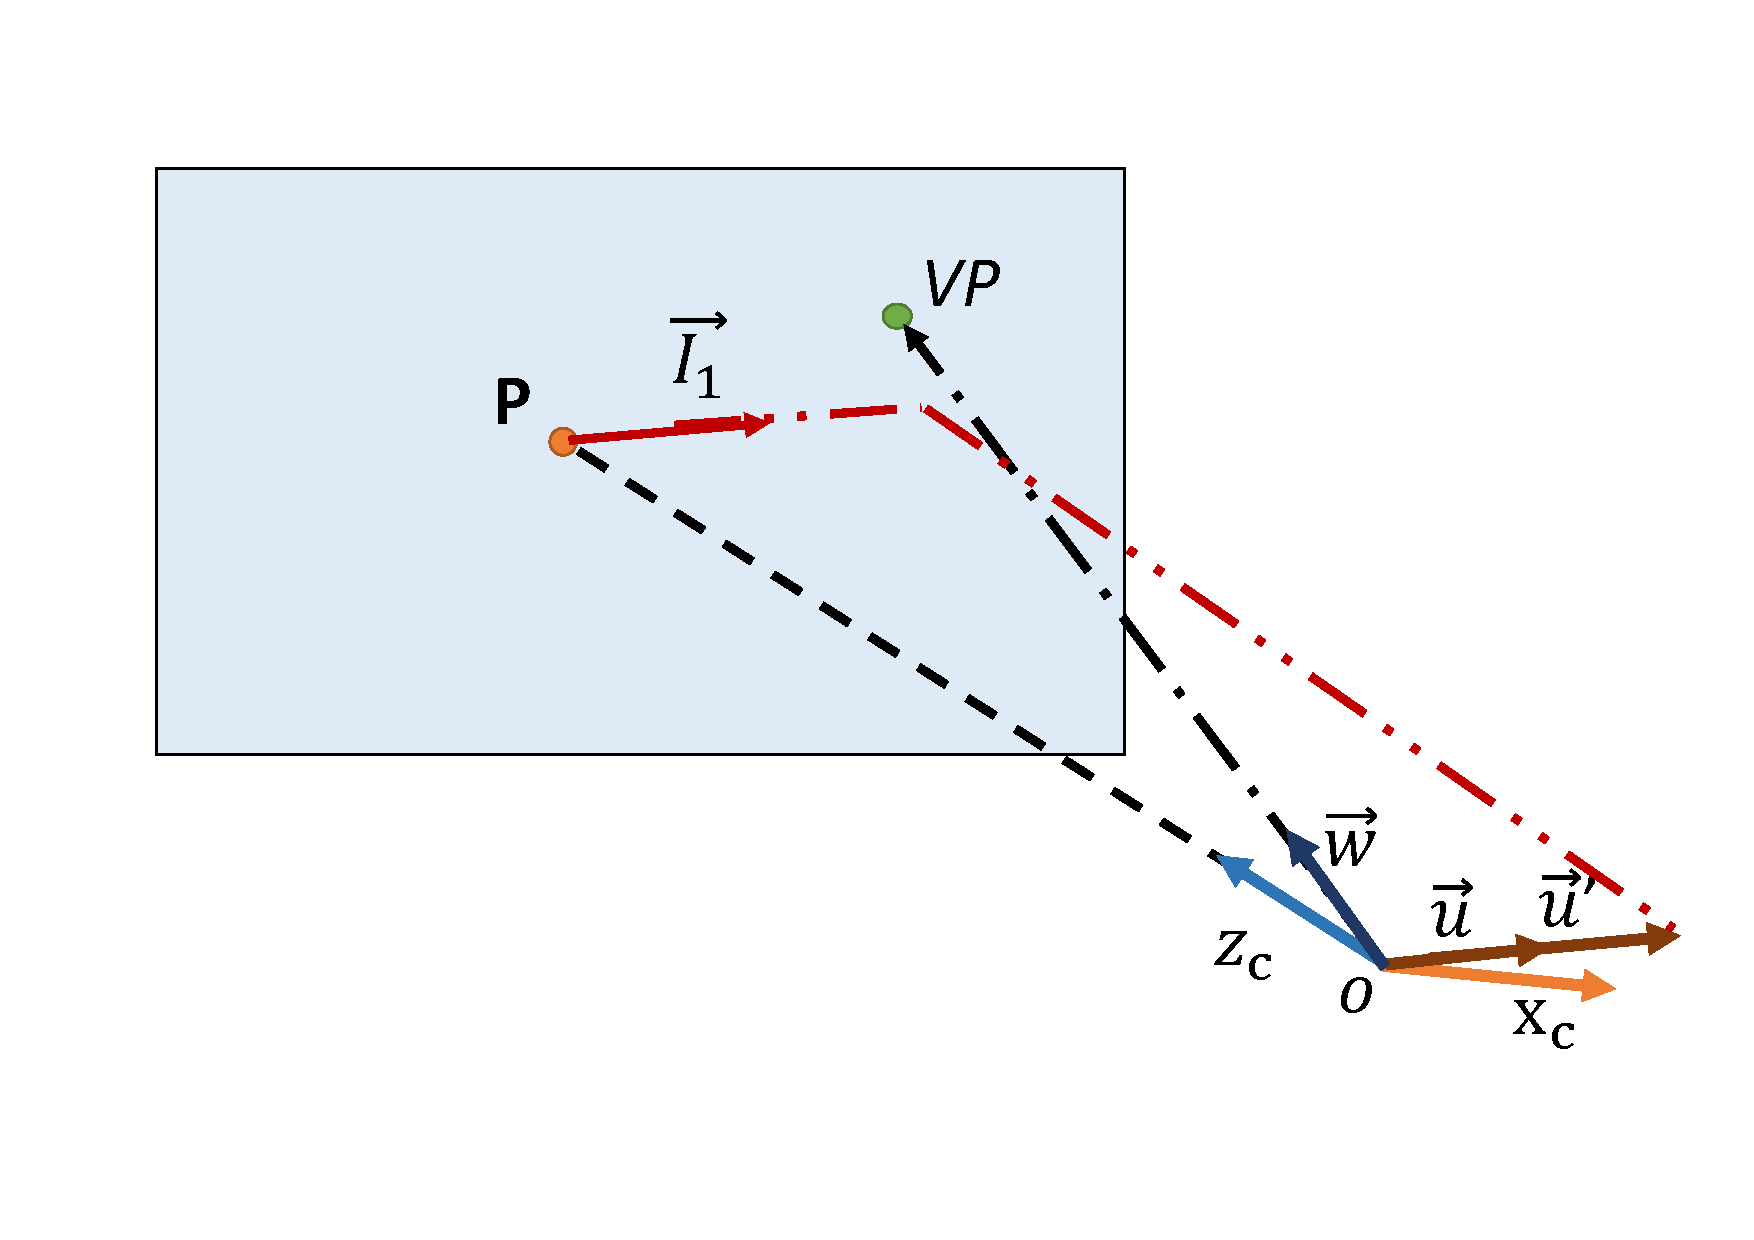
\includegraphics[scale=0.5]{Chapter03/Images/twoInfiniteVPOneFVPH.pdf}
\caption{ $\vec{u}$ estimation from the infinite vanishing points.}
\label{fig:3_unpuntoH}
\end{figure}

Similar procedures can be used for $\vec{v}' = (I_{2_x}, I_{2_y},v_{z}')$ (see Figure \ref{fig:3_unpuntoV}), thus

\begin{equation}
	\label{PlanoV}
	v_{z}'=\frac{I_{2_x}w_{x}'+ I_{2_y}w_{y}'}{f}
\end{equation}

\begin{figure}[h]
\centering
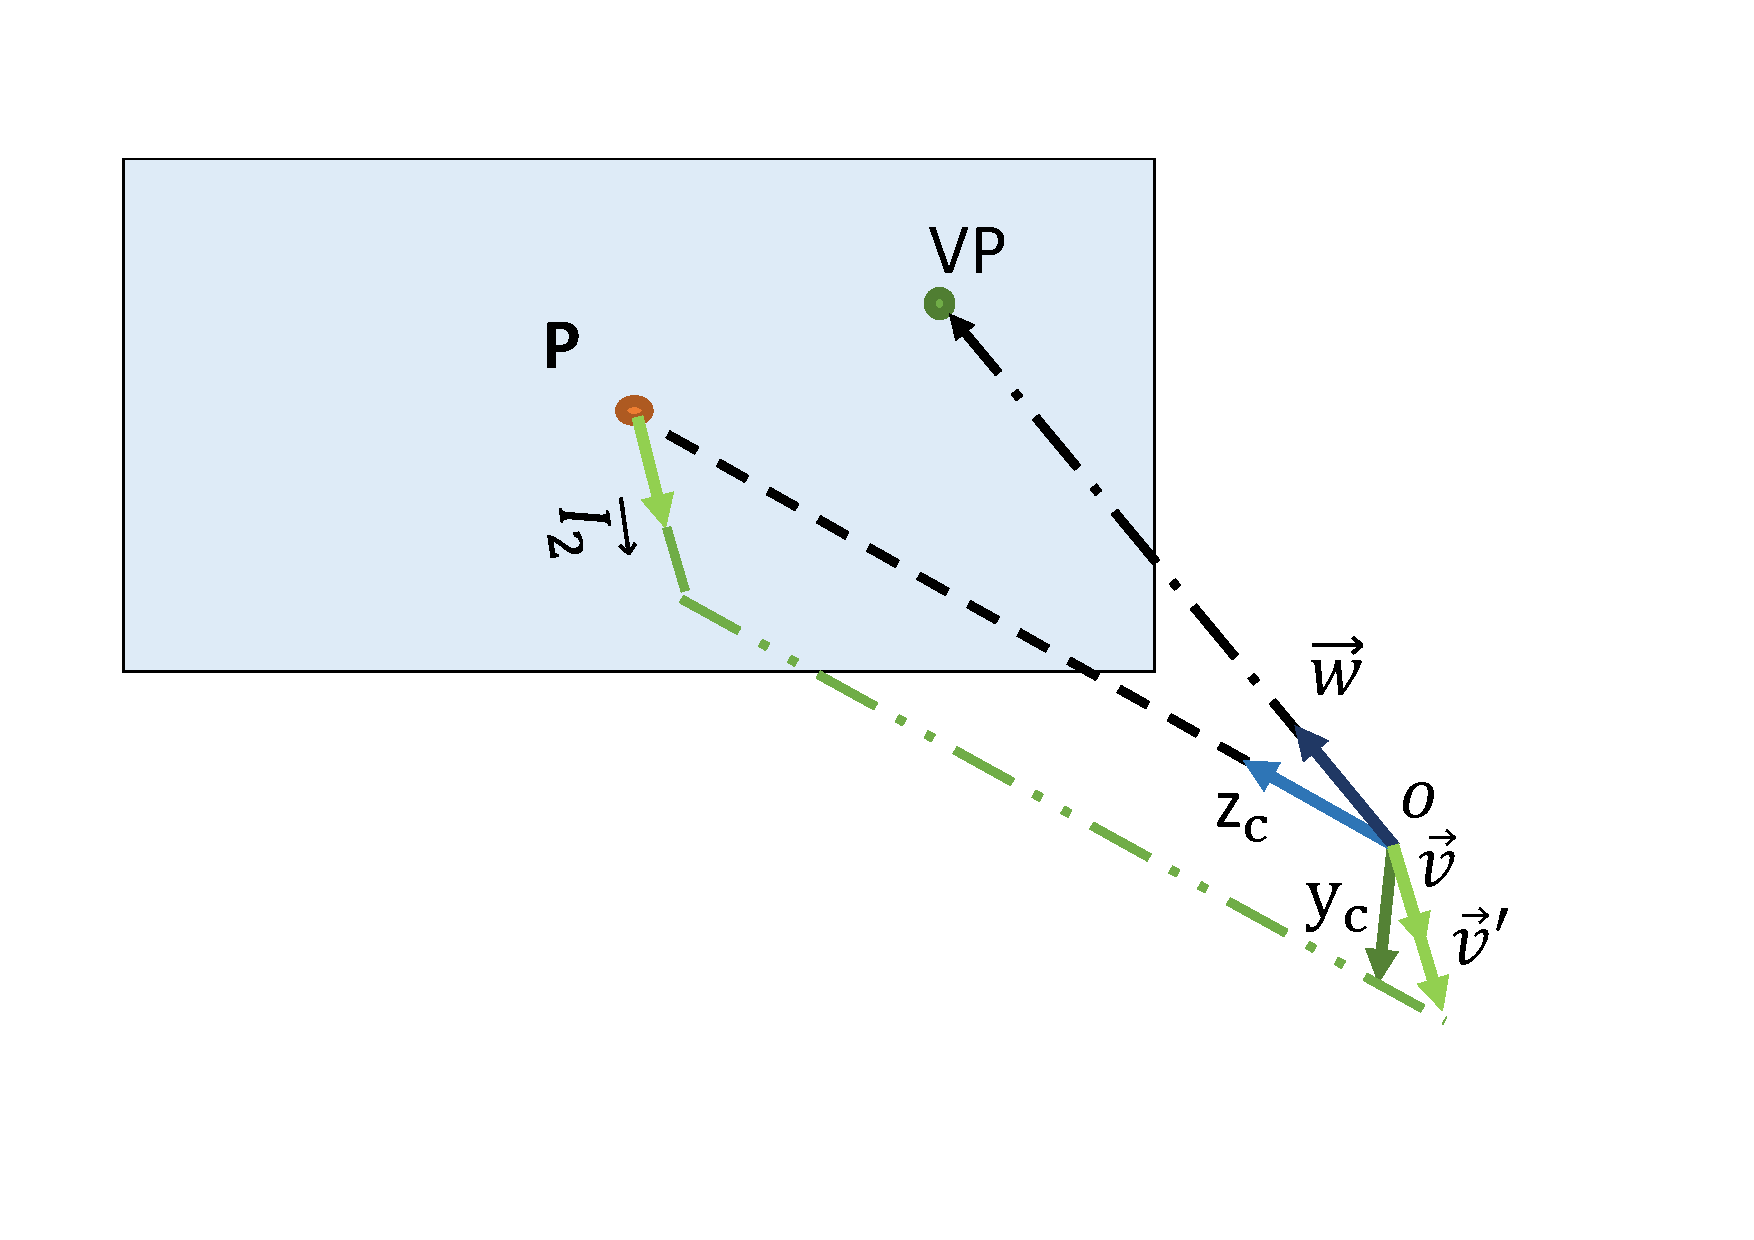
\includegraphics[scale=0.5]{Chapter03/Images/twoInfiniteVPOneFVPV.pdf}
\caption{$\vec{v}$ estimation from  the infinite vanishing points.}
\label{fig:3_unpuntoV}
\end{figure}

Typically the vertical lines are plenty and more precise in
many images, so it retains $\vec{v}'$ and $\vec{w}'$ and compute $\vec{u}'$ using a
cross product, $\vec{u}'= \vec{v}'\times \vec{w}'$. The rotation matrix of the camera $R= (\vec{u},\vec{v},\vec{w})$ from
 Eq. (\ref{CameraMatrix}) which meets the conditions from Eq. (\ref{VectorOrto}) is
obtained by normalizing $\vec{u}'$, $\vec{v}'$ and $\vec{w}'$.


\subsection{Principal lines estimation}

color{blue}

Once the camera rotation matrix obtained, fusing this information with $ L_v $,  $ L_h $ and  $ L_d $ thus, the principal lines of the corridor (corners of the the corridor) could be estimated. The algorithm results in  four new subsets (quadrants 1,2,3,4) relatives with to the vanishing point and the rotation matrix. Therefore, the information in each quadrant
is useful to find the main line of each subset. Each subset of lines contains the beginning and end point of each line as well as its inclination and its length.  \vskip 0.2cm

\color{magenta}

The principal lines which are in the border of the right wall-ceiling $L_{Q_1}$, right wall-floor $L_{Q_2}$,
left wall-ceiling $L_{Q_3}$ and left wall-floor $L_{Q_4}$ are depicted in Fig \ref{fig:VisionAlgoritm}.  \vskip 0.2cm

% \subsubsection{Generalized least squares fitting}

%{\footnotesize
%      \begin{tabular}{p{0.6\textwidth} p{0.4\textwidth}}
	%  \begin{itemize}
%     \item Let  $X_1=(x_1,x_2,...,x_n)^T$ and $Y_1=(y_1,y_2,...,y_n)^T$. Define a new $2\times n$ matrix $X=(X_1, Y_1)^T$.
%    {\tiny

   \begin{equation*}
 C_m\equiv \begin{bmatrix}%\dfrac{1}{2}XX^T=
     \omega_n \sum x_n^2   &  \omega_n \sum x_n y_n \\
     \omega_n \sum x_n y_n &  \omega_n \sum y_n^2
    \end{bmatrix}
\end{equation*}
%}

$(x_n,y_n)$ are the initial and final points from each line, $C_m$ represents the covariance matrix, $m$ represents the frames and
\begin{equation*}
 \omega_n=e^{\frac{-0.5 \theta^2}{\sigma^2}}
\end{equation*}
\begin{equation*}
 \theta=\arctan \frac{x_n a_{m-1}+y_n b_{m-1}}{x_n a_{m-1}-y_n b_{m-1}}
\end{equation*}

Where $\omega_n$ is the weight that supply the response variance to a constant value, $a_{m-1}, b_{m-1}$ represents initial line hypothesis and the .


\begin{equation*}
y=LQ_k=-\frac{b_m}{a_m} x
\end{equation*}
where the vector proper  $\alpha=[a_m, b_m]^T$ extracted from $C_m$ represents the principal line of each quadrant with $k=1,2,3,4$.

\color{red}
Sigo sin entender esta ultima parte que me enviaste
podrias explicarlo en espanol?
\color{black}

\subsection{Pose camera estimation}


\color{blue}

Position camera estimation is obtained using the previous results and the relation with the borders of the corridor. Hence, when the camera is in the center of the corridor, there is a collinearity
between the lines $L_{Q_1},L_{Q_3}$ and $L_{Q_2},L_{Q_4}$ that can be expressed as
\begin{eqnarray}
		   CP_{1,3} &=& L_{Q_1}\wedge L_{Q_3} \label{crossLines13} \\
		   CP_{2,4} &= & L_{Q_2}\wedge L_{Q_4} \label{crossLines24}
\end{eqnarray}

The third component of $CP_{1,3}$ and $CP_{2,4}$ supplies the information to obtain the relative camera position and it is given as
\begin{eqnarray}
		y_r=CP_{1,3}-CP_{2,4} \label{relaitve_x} \\
z_r=CP_{1,3}+CP_{2,4} \label{realitive_z}
\end{eqnarray}
where $y_r$ and $z_r$ are the relative position with respect to the center of the corridor. \\

\color{black}

\color{red}
Las figuras que pusiste y como las pusiste no se ven, tienden a confundir y hace mas complicado el asunto para entender, te voy a poner un bosquejo de como quedaria mejor..
para esto necesito una secuencia de estas figuras separadas (cada figura separada..)
\color{blue}

\section{Numerical validation}
%

The previous algorithm for pose estimation was firstly tested off-line. For corroborating equations (\ref{crossLines13}) and (\ref{crossLines24}) a sequence of images where taken with specified  movements as shown in Figures \ref{camera up and down} and \ref{camera right and left}.

\begin{figure} [h!]
\centering
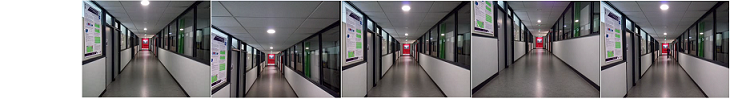
\includegraphics[scale=0.5]{Chapter03/Images/CentreFrames_m.png}
\caption{Pictures with a camera in the middle of a corridor. The test was: 1) stay at the middle, 2) move up, 3) returns to the middle, 4) move down and 5) returns to the middle. }
\label{camera up and down}
\end{figure}


\begin{figure} [h!]
\centering
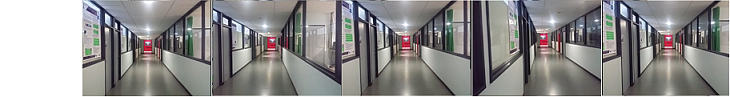
\includegraphics[scale=0.5]{Chapter03/Images/Lateral_m.png}
\caption{Pictures with a camera in the middle of a corridor. The test was: 1) stay at the middle, 2) move rigth, 3) returns to the middle, 4) move left and 5) returns to the middle. }
\label{camera right and left}
\end{figure}

The experiment was to place the camera in the middle of the corridor and moves it firstly up and down (Figure \ref{camera up and down}) and after right and left (Figure \ref{camera right and left}). These movements can be represented via principal lines in the image and observed graphically in Figures  \ref{fig:CentreFrames} and \ref{fig:lateralFRames}, where the cross product between $L_{Q_i}$ are represented, see (\ref{crossLines13}) and (\ref{crossLines24}). On one hand, notice for example from Figure \ref{fig:CentreFrames}  that both cross products have the same behavior and when if the camera is moved up the lines representing $L_{Q_1}\wedge L_{Q_3}$  and $L_{Q_4}\wedge L_{Q_2}$ increase and when the camera is moved down they decrease, representing then the good camera's behavior. On the other hand, when the camera is moved right and left, then the cross product between $L_{Q_1}\wedge L_{Q_3}$  and $L_{Q_4}\wedge L_{Q_2}$ are different (see Figure  \ref{fig:lateralFRames}), nevertheless this information gives necessary data to estimate the $y$ position, as can be seen in Figure  \ref{fig:XYlateral}. Observe in this figure that when the camera is moved right the $y$ estimation is negative and if it is moved left, then a $y$ positive response is obtained. In addition note that $z$ estimation remains quasi-constant. Similarly for Figure \ref{fig:XYcentre} where with the up and down camera's movements the $z$ state is estimated, observe also that $y$ estimation is also quasi-constant.



\begin{figure}[h!]
        \centering
        % This file was created by matlab2tikz.
% Minimal pgfplots version: 1.3
%
%The latest updates can be retrieved from
%  http://www.mathworks.com/matlabcentral/fileexchange/22022-matlab2tikz
%where you can also make suggestions and rate matlab2tikz.
%
\definecolor{mycolor1}{rgb}{0.00000,0.44700,0.74100}%
\definecolor{mycolor2}{rgb}{0.85000,0.32500,0.09800}%
%
\begin{tikzpicture}

\begin{axis}[%
width=6.656442cm,
height=3cm,
at={(0cm,0cm)},
scale only axis,
xmin=0,
xmax=60,
xlabel={Time (sec)},
xmajorgrids,
ymin=-0.3,
ymax=0.5,
ylabel={Cross product},
ymajorgrids,
legend style={legend columns=2,legend cell align=left,align=left,draw=white!15!black}
]
\addplot [color=mycolor1,solid,line width=2.0pt]
  table[row sep=crcr]{%
0	0\\
0.199335548172757	0.030742027925972\\
0.398671096345515	0.0828735307141348\\
0.598006644518272	0.105081321825358\\
0.79734219269103	0.138826415767478\\
0.996677740863787	0.158012182380284\\
1.19601328903654	0.165318336971575\\
1.3953488372093	0.129759187651805\\
1.59468438538206	0.153461059573169\\
1.79401993355482	0.162469237192847\\
1.99335548172757	0.167889162514036\\
2.19269102990033	0.175363911624859\\
2.39202657807309	0.17679802060079\\
2.59136212624585	0.169046976759301\\
2.7906976744186	0.17803807773658\\
2.99003322259136	0.17865142111461\\
3.18936877076412	0.180553164243146\\
3.38870431893688	0.187710505101491\\
3.58803986710963	0.204041035478399\\
3.78737541528239	0.21217945191349\\
3.98671096345515	0.21305849534408\\
4.18604651162791	0.211274427028537\\
4.38538205980066	0.208293620013859\\
4.58471760797342	0.20836783661539\\
4.78405315614618	0.208628644841035\\
4.98338870431894	0.208369223901828\\
5.18272425249169	0.206154168791621\\
5.38205980066445	0.21778747263864\\
5.58139534883721	0.211650949117691\\
5.78073089700997	0.210224040265121\\
5.98006644518272	0.216316680182076\\
6.17940199335548	0.212784544860855\\
6.37873754152824	0.216163792212759\\
6.578073089701	0.210087929923006\\
6.77740863787375	0.196315112872329\\
6.97674418604651	0.197105507459289\\
7.17607973421927	0.197806072188377\\
7.37541528239203	0.193373638163163\\
7.57475083056478	0.208069099458681\\
7.77408637873754	0.208034793813171\\
7.9734219269103	0.198240381391177\\
8.17275747508306	0.195685221835226\\
8.37209302325581	0.198911960913538\\
8.57142857142857	0.19944310829398\\
8.77076411960133	0.200307530669613\\
8.97009966777409	0.201433223855905\\
9.16943521594684	0.200608875718738\\
9.3687707641196	0.209704024239964\\
9.56810631229236	0.209636210457107\\
9.76744186046512	0.206945066931917\\
9.96677740863787	0.20756166503172\\
10.1661129568106	0.211824702244533\\
10.3654485049834	0.214729736631606\\
10.5647840531561	0.218446630875855\\
10.7641196013289	0.215449324758097\\
10.9634551495017	0.212325909892533\\
11.1627906976744	0.221127132960991\\
11.3621262458472	0.230712638671687\\
11.5614617940199	0.244434338600201\\
11.7607973421927	0.256643111495394\\
11.9601328903654	0.270713831033366\\
12.1594684385382	0.291476166526801\\
12.358803986711	0.310759262817296\\
12.5581395348837	0.32485284027707\\
12.7574750830565	0.346592051833787\\
12.9568106312292	0.369733610076934\\
13.156146179402	0.387575727549183\\
13.3554817275748	0.400630217873027\\
13.5548172757475	0.406061953187462\\
13.7541528239203	0.4202093386277\\
13.953488372093	0.426108587752899\\
14.1528239202658	0.433045756421874\\
14.3521594684385	0.440076903749821\\
14.5514950166113	0.444816326368204\\
14.7508305647841	0.450248529944735\\
14.9501661129568	0.452032845365701\\
15.1495016611296	0.456702468586884\\
15.3488372093023	0.457721551086022\\
15.5481727574751	0.456476945481678\\
15.7475083056478	0.456228382158606\\
15.9468438538206	0.457351532254795\\
16.1461794019934	0.458873391847378\\
16.3455149501661	0.460155924541988\\
16.5448504983389	0.463836678313106\\
16.7441860465116	0.46708914589731\\
16.9435215946844	0.467229370585945\\
17.1428571428571	0.468814394298497\\
17.3421926910299	0.467151525259722\\
17.5415282392027	0.469992125696965\\
17.7408637873754	0.470488153561163\\
17.9401993355482	0.47133828366119\\
18.1395348837209	0.4712136054494\\
18.3388704318937	0.473197952459583\\
18.5382059800664	0.473811810239429\\
18.7375415282392	0.473721931121786\\
18.936877076412	0.474306122558772\\
19.1362126245847	0.473769240182764\\
19.3355481727575	0.471807952378505\\
19.5348837209302	0.475075360110677\\
19.734219269103	0.474889855501165\\
19.9335548172757	0.471753722095564\\
20.1328903654485	0.471711717964217\\
20.3322259136213	0.471434487222184\\
20.531561461794	0.471181142315513\\
20.7308970099668	0.471324136765159\\
20.9302325581395	0.47165937825952\\
21.1295681063123	0.471579238738933\\
21.3289036544851	0.471649215234227\\
21.5282392026578	0.471422751723768\\
21.7275747508306	0.471064366542006\\
21.9269102990033	0.471177084730362\\
22.1262458471761	0.476173602152583\\
22.3255813953488	0.476317277665897\\
22.5249169435216	0.476468981081323\\
22.7242524916944	0.474890491991672\\
22.9235880398671	0.485672390921398\\
23.1229235880399	0.481640805503392\\
23.3222591362126	0.481305711319191\\
23.5215946843854	0.479101891431731\\
23.7209302325581	0.477222689645709\\
23.9202657807309	0.46995585831105\\
24.1196013289037	0.470143173565368\\
24.3189368770764	0.471353888074935\\
24.5182724252492	0.474670849246479\\
24.7176079734219	0.474214982532677\\
24.9169435215947	0.473309232825266\\
25.1162790697674	0.4702148595381\\
25.3156146179402	0.466623685141034\\
25.514950166113	0.458434098808722\\
25.7142857142857	0.431922133556878\\
25.9136212624585	0.406036866021997\\
26.1129568106312	0.38039995269299\\
26.312292358804	0.356831546083206\\
26.5116279069767	0.322200657313163\\
26.7109634551495	0.305814299966114\\
26.9102990033223	0.280394856478819\\
27.109634551495	0.263781848291225\\
27.3089700996678	0.248955514608588\\
27.5083056478405	0.236306847625229\\
27.7076411960133	0.226281537481772\\
27.906976744186	0.222261370563225\\
28.1063122923588	0.224721022706015\\
28.3056478405316	0.22476533346158\\
28.5049833887043	0.219702791930158\\
28.7043189368771	0.218639125249466\\
28.9036544850498	0.213235288983912\\
29.1029900332226	0.212913375488299\\
29.3023255813953	0.21228176757624\\
29.5016611295681	0.223800534132015\\
29.7009966777409	0.226901606259314\\
29.9003322259136	0.221722406316364\\
30.0996677740864	0.225702789436084\\
30.2990033222591	0.228714968858014\\
30.4983388704319	0.218398774482463\\
30.6976744186047	0.213802060701838\\
30.8970099667774	0.225847310857305\\
31.0963455149502	0.227346203360617\\
31.2956810631229	0.216690547489862\\
31.4950166112957	0.216552662799759\\
31.6943521594684	0.217670360719735\\
31.8936877076412	0.189999617580706\\
32.093023255814	0.19020693329187\\
32.2923588039867	0.20531608916418\\
32.4916943521595	0.201752114776826\\
32.6910299003322	0.189051967535848\\
32.890365448505	0.186402236710532\\
33.0897009966777	0.195223273001069\\
33.2890365448505	0.21553877298573\\
33.4883720930233	0.199105585068201\\
33.687707641196	0.205330469090425\\
33.8870431893688	0.20231250412812\\
34.0863787375415	0.204315298733265\\
34.2857142857143	0.213043572400633\\
34.485049833887	0.216381165891312\\
34.6843853820598	0.214338312518101\\
34.8837209302326	0.190891845755397\\
35.0830564784053	0.169045388129524\\
35.2823920265781	0.117970056131066\\
35.4817275747508	0.0618122169285922\\
35.6810631229236	0.0212892341015012\\
35.8803986710963	-0.021581250796285\\
36.0797342192691	-0.0407628403912041\\
36.2790697674419	-0.0643765588041649\\
36.4784053156146	-0.0845714012217986\\
36.6777408637874	-0.114381902194977\\
36.8770764119601	-0.123194462033602\\
37.0764119601329	-0.14726030403955\\
37.2757475083056	-0.16825262185245\\
37.4750830564784	-0.187557341614786\\
37.6744186046512	-0.19123943099753\\
37.8737541528239	-0.20267788063962\\
38.0730897009967	-0.211819315074755\\
38.2724252491694	-0.217778009185701\\
38.4717607973422	-0.228140241975077\\
38.671096345515	-0.217250594700689\\
38.8704318936877	-0.226107038531323\\
39.0697674418605	-0.23101328496671\\
39.2691029900332	-0.236516404359276\\
39.468438538206	-0.241075317536677\\
39.6677740863787	-0.244948723856249\\
39.8671096345515	-0.247255132191605\\
40.0664451827243	-0.245453814770265\\
40.265780730897	-0.246176164527333\\
40.4651162790698	-0.247822375278133\\
40.6644518272425	-0.249055730427652\\
40.8637873754153	-0.250090430167425\\
41.063122923588	-0.263017147931831\\
41.2624584717608	-0.263663827137829\\
41.4617940199336	-0.242798079796263\\
41.6611295681063	-0.24919543837436\\
41.8604651162791	-0.256558503461077\\
42.0598006644518	-0.259350205694448\\
42.2591362126246	-0.260856593203861\\
42.4584717607973	-0.259369184086433\\
42.6578073089701	-0.260847042991638\\
42.8571428571429	-0.265856079830801\\
43.0564784053156	-0.267909493358909\\
43.2558139534884	-0.249627090506112\\
43.4551495016611	-0.252631241082031\\
43.6544850498339	-0.24767615356644\\
43.8538205980066	-0.253337795568863\\
44.0531561461794	-0.250813819942353\\
44.2524916943522	-0.254503959520435\\
44.4518272425249	-0.256560896988312\\
44.6511627906977	-0.256939124807369\\
44.8504983388704	-0.260644196262074\\
45.0498338870432	-0.26467599272932\\
45.2491694352159	-0.270060067743338\\
45.4485049833887	-0.272537541860207\\
45.6478405315615	-0.274229327053171\\
45.8471760797342	-0.275545675048239\\
46.046511627907	-0.279129379972995\\
46.2458471760797	-0.281198619991069\\
46.4451827242525	-0.28133388193592\\
46.6445182724253	-0.284666226184072\\
46.843853820598	-0.269029365875755\\
47.0431893687708	-0.247307299970423\\
47.2425249169435	-0.235748069151903\\
47.4418604651163	-0.225715507665264\\
47.641196013289	-0.225238129680491\\
47.8405315614618	-0.225433256373713\\
48.0398671096346	-0.225339898102067\\
48.2392026578073	-0.217279286472469\\
48.4385382059801	-0.21950817849527\\
48.6378737541528	-0.21034184070411\\
48.8372093023256	-0.212044448467703\\
49.0365448504983	-0.222970250691113\\
49.2358803986711	-0.239279839462634\\
49.4352159468439	-0.229448609262718\\
49.6345514950166	-0.227709614278369\\
49.8338870431894	-0.161321648091734\\
50.0332225913621	-0.125025189719276\\
50.2325581395349	-0.0836592328544258\\
50.4318936877076	-0.0398627348046633\\
50.6312292358804	0.00644523607091106\\
50.8305647840532	0.0489271269236699\\
51.0299003322259	0.0817933479629508\\
51.2292358803987	0.116461406303344\\
51.4285714285714	0.133142431877358\\
51.6279069767442	0.141687609276178\\
51.8272425249169	0.143640859102146\\
52.0265780730897	0.163266584448222\\
52.2259136212625	0.167208817911571\\
52.4252491694352	0.170736927140942\\
52.624584717608	0.178133943399358\\
52.8239202657807	0.180061169482605\\
53.0232558139535	0.180927859896376\\
53.2225913621263	0.181934431053367\\
53.421926910299	0.188007236741809\\
53.6212624584718	0.193329091764933\\
53.8205980066445	0.193715212411015\\
54.0199335548173	0.193450778499299\\
54.21926910299	0.193539146654546\\
54.4186046511628	0.183228797260322\\
54.6179401993356	0.18367127988381\\
54.8172757475083	0.182204850007427\\
55.0166112956811	0.192454709402846\\
55.2159468438538	0.195686603320542\\
55.4152823920266	0.185684729861345\\
55.6146179401993	0.190869703698701\\
55.8139534883721	0.195644283409796\\
56.0132890365449	0.194616307400244\\
56.2126245847176	0.201526368934063\\
56.4119601328904	0.199051661999297\\
56.6112956810631	0.198620778169795\\
56.8106312292359	0.196725532921711\\
57.0099667774086	0.193020051971268\\
57.2093023255814	0.191649981814679\\
57.4086378737542	0.195882780971597\\
57.6079734219269	0.202607878832124\\
57.8073089700997	0.197014402839495\\
58.0066445182724	0.19407472768477\\
58.2059800664452	0.194624427427319\\
58.4053156146179	0.194431061787678\\
58.6046511627907	0.200303432988159\\
58.8039867109635	0.200403545770639\\
59.0033222591362	0.20509426583411\\
59.202657807309	0.208041508591756\\
59.4019933554817	0.205603969967094\\
59.6013289036545	0.211738682009683\\
59.8006644518272	0.211399667764344\\
};
\addlegendentry{$\text{L}_{\text{Q}_\text{1}}\wedge\text{L}_{\text{Q}_\text{3}}$};

\addplot [color=mycolor2,dashed,line width=2.0pt]
  table[row sep=crcr]{%
0	0\\
0.199335548172757	0.0320626091915426\\
0.398671096345515	0.0817511843045116\\
0.598006644518272	0.127257203409701\\
0.79734219269103	0.154878094363065\\
0.996677740863787	0.179061563427889\\
1.19601328903654	0.185412066139698\\
1.3953488372093	0.186713908020985\\
1.59468438538206	0.200172253811674\\
1.79401993355482	0.201408954219292\\
1.99335548172757	0.20493449428673\\
2.19269102990033	0.205666676396152\\
2.39202657807309	0.206091359201615\\
2.59136212624585	0.206554749313233\\
2.7906976744186	0.211245329020206\\
2.99003322259136	0.211004873573202\\
3.18936877076412	0.21437742267165\\
3.38870431893688	0.216087694229007\\
3.58803986710963	0.21883893501534\\
3.78737541528239	0.218787320906457\\
3.98671096345515	0.219100453366994\\
4.18604651162791	0.218828742295831\\
4.38538205980066	0.224891894713642\\
4.58471760797342	0.224084047829433\\
4.78405315614618	0.221608644407124\\
4.98338870431894	0.218141591611892\\
5.18272425249169	0.215973212731868\\
5.38205980066445	0.214869476282882\\
5.58139534883721	0.214832736484727\\
5.78073089700997	0.214520416483156\\
5.98006644518272	0.214318637089189\\
6.17940199335548	0.214378454531542\\
6.37873754152824	0.213806510019757\\
6.578073089701	0.213767209496671\\
6.77740863787375	0.212851766144994\\
6.97674418604651	0.213635770208655\\
7.17607973421927	0.214117975182495\\
7.37541528239203	0.213995210047199\\
7.57475083056478	0.213436457093262\\
7.77408637873754	0.213404921652426\\
7.9734219269103	0.213259081211162\\
8.17275747508306	0.210778414051719\\
8.37209302325581	0.210792658205226\\
8.57142857142857	0.211480669231338\\
8.77076411960133	0.246138702289899\\
8.97009966777409	0.241421057178173\\
9.16943521594684	0.23773060414665\\
9.3687707641196	0.234113319797148\\
9.56810631229236	0.231911115413748\\
9.76744186046512	0.229887654146903\\
9.96677740863787	0.227800908991243\\
10.1661129568106	0.225846015817527\\
10.3654485049834	0.224466288487356\\
10.5647840531561	0.223095742944597\\
10.7641196013289	0.222260662612162\\
10.9634551495017	0.222841013927408\\
11.1627906976744	0.227340962641489\\
11.3621262458472	0.236956035470035\\
11.5614617940199	0.250237205281052\\
11.7607973421927	0.283528505930164\\
11.9601328903654	0.303650126242148\\
12.1594684385382	0.315448923935091\\
12.358803986711	0.326677526241795\\
12.5581395348837	0.347620970146806\\
12.7574750830565	0.36752847063599\\
12.9568106312292	0.378155959398808\\
13.156146179402	0.388537615145302\\
13.3554817275748	0.392512683027438\\
13.5548172757475	0.405576971942509\\
13.7541528239203	0.413700981546986\\
13.953488372093	0.419426281941872\\
14.1528239202658	0.427594729790868\\
14.3521594684385	0.437246896869441\\
14.5514950166113	0.450253300202354\\
14.7508305647841	0.464536511266053\\
14.9501661129568	0.470012404887887\\
15.1495016611296	0.47189344984303\\
15.3488372093023	0.474640714579043\\
15.5481727574751	0.475999724330138\\
15.7475083056478	0.470611422487283\\
15.9468438538206	0.474761082614527\\
16.1461794019934	0.476899066937246\\
16.3455149501661	0.476217715416071\\
16.5448504983389	0.474470001404674\\
16.7441860465116	0.474082013352342\\
16.9435215946844	0.471938428869725\\
17.1428571428571	0.467612304892456\\
17.3421926910299	0.472623837455728\\
17.5415282392027	0.471387909977419\\
17.7408637873754	0.469725743834744\\
17.9401993355482	0.468180525944768\\
18.1395348837209	0.468221464957505\\
18.3388704318937	0.466583711920482\\
18.5382059800664	0.467159986560546\\
18.7375415282392	0.466323841682952\\
18.936877076412	0.465295250371364\\
19.1362126245847	0.46429627027929\\
19.3355481727575	0.465701148468471\\
19.5348837209302	0.467100654110654\\
19.734219269103	0.469453919774675\\
19.9335548172757	0.474120692359259\\
20.1328903654485	0.473870660381315\\
20.3322259136213	0.470432692934215\\
20.531561461794	0.467806937713826\\
20.7308970099668	0.470353738651148\\
20.9302325581395	0.473318183307137\\
21.1295681063123	0.473273428823387\\
21.3289036544851	0.468577266163835\\
21.5282392026578	0.466026366882535\\
21.7275747508306	0.462070486998969\\
21.9269102990033	0.459662105391332\\
22.1262458471761	0.458923207735633\\
22.3255813953488	0.458158771321329\\
22.5249169435216	0.453915414368753\\
22.7242524916944	0.455986483906308\\
22.9235880398671	0.455834987337035\\
23.1229235880399	0.455744716884746\\
23.3222591362126	0.455774084724335\\
23.5215946843854	0.454746668633451\\
23.7209302325581	0.454412158586011\\
23.9202657807309	0.454252840232174\\
24.1196013289037	0.459016669187824\\
24.3189368770764	0.458486528852053\\
24.5182724252492	0.456755022692895\\
24.7176079734219	0.456654076710454\\
24.9169435215947	0.454987235914474\\
25.1162790697674	0.457482822558321\\
25.3156146179402	0.448328684676984\\
25.514950166113	0.437408133237098\\
25.7142857142857	0.429611692237303\\
25.9136212624585	0.411043810894273\\
26.1129568106312	0.382575060219923\\
26.312292358804	0.352513142210869\\
26.5116279069767	0.326688852066983\\
26.7109634551495	0.304112147295015\\
26.9102990033223	0.282025284854331\\
27.109634551495	0.266611214942692\\
27.3089700996678	0.2562916461232\\
27.5083056478405	0.246599528301404\\
27.7076411960133	0.243527454639695\\
27.906976744186	0.241790371632504\\
28.1063122923588	0.240348524556144\\
28.3056478405316	0.238757039457458\\
28.5049833887043	0.252554379755047\\
28.7043189368771	0.248279152556026\\
28.9036544850498	0.243686657069989\\
29.1029900332226	0.241266806044097\\
29.3023255813953	0.238988137712187\\
29.5016611295681	0.237955806271094\\
29.7009966777409	0.238708093532441\\
29.9003322259136	0.237365627514156\\
30.0996677740864	0.235764489654768\\
30.2990033222591	0.23421284259758\\
30.4983388704319	0.232210821850323\\
30.6976744186047	0.230656306656538\\
30.8970099667774	0.230484754444466\\
31.0963455149502	0.229447324896434\\
31.2956810631229	0.226982858920684\\
31.4950166112957	0.222949395854119\\
31.6943521594684	0.222477392749945\\
31.8936877076412	0.21723769049055\\
32.093023255814	0.216739632931268\\
32.2923588039867	0.216784460731293\\
32.4916943521595	0.216400153537603\\
32.6910299003322	0.215973899128233\\
32.890365448505	0.215459023405163\\
33.0897009966777	0.215440567021171\\
33.2890365448505	0.223128934585933\\
33.4883720930233	0.222208330481669\\
33.687707641196	0.221771538333541\\
33.8870431893688	0.219866907863976\\
34.0863787375415	0.219791047886523\\
34.2857142857143	0.219793881559957\\
34.485049833887	0.219596082300113\\
34.6843853820598	0.218806705617196\\
34.8837209302326	0.211136896685235\\
35.0830564784053	0.185722460245505\\
35.2823920265781	0.151147760970004\\
35.4817275747508	0.100016059177831\\
35.6810631229236	0.0446807030055201\\
35.8803986710963	0.0655724471034565\\
36.0797342192691	0.0160822779959248\\
36.2790697674419	-0.0216478579850808\\
36.4784053156146	-0.0584967055520748\\
36.6777408637874	-0.0851517401062519\\
36.8770764119601	-0.10160898273506\\
37.0764119601329	-0.113724411683194\\
37.2757475083056	-0.13267880360071\\
37.4750830564784	-0.14168608785018\\
37.6744186046512	-0.15377612412339\\
37.8737541528239	-0.161571624709748\\
38.0730897009967	-0.171065255891224\\
38.2724252491694	-0.179467436496735\\
38.4717607973422	-0.184614051280749\\
38.671096345515	-0.194463573438089\\
38.8704318936877	-0.197962840153099\\
39.0697674418605	-0.198830905789283\\
39.2691029900332	-0.20315813009051\\
39.468438538206	-0.207442191143203\\
39.6677740863787	-0.208292920236624\\
39.8671096345515	-0.2079207696927\\
40.0664451827243	-0.211377893238493\\
40.265780730897	-0.213102293138477\\
40.4651162790698	-0.213729931604371\\
40.6644518272425	-0.215499054703499\\
40.8637873754153	-0.214755221286152\\
41.063122923588	-0.215419827508301\\
41.2624584717608	-0.219886874688999\\
41.4617940199336	-0.221351351082579\\
41.6611295681063	-0.223319165451339\\
41.8604651162791	-0.224894029267765\\
42.0598006644518	-0.228584877257247\\
42.2591362126246	-0.230414149355335\\
42.4584717607973	-0.229187553308355\\
42.6578073089701	-0.233114418046791\\
42.8571428571429	-0.231148989983818\\
43.0564784053156	-0.230874041204472\\
43.2558139534884	-0.234404718799207\\
43.4551495016611	-0.230970347513089\\
43.6544850498339	-0.234018744118853\\
43.8538205980066	-0.232444624210312\\
44.0531561461794	-0.235202144840751\\
44.2524916943522	-0.235603608313914\\
44.4518272425249	-0.235627435706585\\
44.6511627906977	-0.235481614716005\\
44.8504983388704	-0.236822095402776\\
45.0498338870432	-0.234817327564808\\
45.2491694352159	-0.234815706659782\\
45.4485049833887	-0.235109964031422\\
45.6478405315615	-0.236713308135239\\
45.8471760797342	-0.237615507114977\\
46.046511627907	-0.239699646987028\\
46.2458471760797	-0.238530659543076\\
46.4451827242525	-0.239372507100505\\
46.6445182724253	-0.236080557181417\\
46.843853820598	-0.241092404422802\\
47.0431893687708	-0.242326750702718\\
47.2425249169435	-0.242958634719738\\
47.4418604651163	-0.243912777442231\\
47.641196013289	-0.240389941192291\\
47.8405315614618	-0.240139204373078\\
48.0398671096346	-0.236927121663719\\
48.2392026578073	-0.236016440709259\\
48.4385382059801	-0.235909495186352\\
48.6378737541528	-0.240482178542547\\
48.8372093023256	-0.240865060272296\\
49.0365448504983	-0.241668325930895\\
49.2358803986711	-0.238155732766004\\
49.4352159468439	-0.239017448284166\\
49.6345514950166	-0.222279129816369\\
49.8338870431894	-0.213714521310704\\
50.0332225913621	-0.162956466487615\\
50.2325581395349	-0.108079023397395\\
50.4318936877076	-0.0480925055210287\\
50.6312292358804	0.00334827215358234\\
50.8305647840532	0.0488704752020988\\
51.0299003322259	0.0863004748789584\\
51.2292358803987	0.114994029767972\\
51.4285714285714	0.1337720227875\\
51.6279069767442	0.148199859087158\\
51.8272425249169	0.158296933812294\\
52.0265780730897	0.169082519827637\\
52.2259136212625	0.17901412125142\\
52.4252491694352	0.181564813613354\\
52.624584717608	0.186690691516834\\
52.8239202657807	0.187998169175694\\
53.0232558139535	0.190346770789243\\
53.2225913621263	0.194783610169169\\
53.421926910299	0.196471812981709\\
53.6212624584718	0.200490000306102\\
53.8205980066445	0.200993769937054\\
54.0199335548173	0.200941120931024\\
54.21926910299	0.20087923051326\\
54.4186046511628	0.200898719888252\\
54.6179401993356	0.215031986916089\\
54.8172757475083	0.213221157392125\\
55.0166112956811	0.21270209739039\\
55.2159468438538	0.210586415777973\\
55.4152823920266	0.20851537902506\\
55.6146179401993	0.207886036495909\\
55.8139534883721	0.205373533673452\\
56.0132890365449	0.204406018843032\\
56.2126245847176	0.203790598773077\\
56.4119601328904	0.202000734044225\\
56.6112956810631	0.199944163914177\\
56.8106312292359	0.19829265072892\\
57.0099667774086	0.196510800833752\\
57.2093023255814	0.194867939626268\\
57.4086378737542	0.193879454244979\\
57.6079734219269	0.193734559392094\\
57.8073089700997	0.191891387441721\\
58.0066445182724	0.191355892470336\\
58.2059800664452	0.191103449276677\\
58.4053156146179	0.189713977600956\\
58.6046511627907	0.189008442349799\\
58.8039867109635	0.188541898281262\\
59.0033222591362	0.242105429389832\\
59.202657807309	0.225698828894778\\
59.4019933554817	0.216938757524525\\
59.6013289036545	0.209052829599811\\
59.8006644518272	0.204755319843383\\
};
\addlegendentry{$\text{L}_{\text{Q}_\text{4}}\wedge\text{L}_{\text{Q}_\text{2}}$};

\end{axis}
\end{tikzpicture}%
   \caption{Frames position and cross product, the camera is moving up and down}
    \label{fig:CentreFrames}
 \end{figure}
   
      
\begin{figure}[h!]
        \centering
      % This file was created by matlab2tikz.
% Minimal pgfplots version: 1.3
%
%The latest updates can be retrieved from
%  http://www.mathworks.com/matlabcentral/fileexchange/22022-matlab2tikz
%where you can also make suggestions and rate matlab2tikz.
%
\definecolor{mycolor1}{rgb}{0.00000,0.44700,0.74100}%
\definecolor{mycolor2}{rgb}{0.85000,0.32500,0.09800}%
%
\begin{tikzpicture}

\begin{axis}[%
width=6.656442cm,
height=3cm,
at={(0cm,0cm)},
scale only axis,
xmin=0,
xmax=60,
xlabel={Time (sec)},
xmajorgrids,
ymin=-0.6,
ymax=1,
ylabel={Relative position},
ymajorgrids,
legend style={legend columns=2,legend cell align=left,align=left,draw=white!15!black}
]
\addplot [color=mycolor1,solid,line width=2.0pt]
  table[row sep=crcr]{%
0	0\\
0.199335548172757	-0.00132058126557062\\
0.398671096345515	0.00112234640962325\\
0.598006644518272	-0.0221758815843431\\
0.79734219269103	-0.0160516785955867\\
0.996677740863787	-0.0210493810476044\\
1.19601328903654	-0.0200937291681225\\
1.3953488372093	-0.0569547203691796\\
1.59468438538206	-0.0467111942385056\\
1.79401993355482	-0.0389397170264447\\
1.99335548172757	-0.0370453317726938\\
2.19269102990033	-0.0303027647712935\\
2.39202657807309	-0.0292933386008251\\
2.59136212624585	-0.0375077725539325\\
2.7906976744186	-0.0332072512836254\\
2.99003322259136	-0.0323534524585916\\
3.18936877076412	-0.033824258428504\\
3.38870431893688	-0.0283771891275158\\
3.58803986710963	-0.0147978995369406\\
3.78737541528239	-0.00660786899296631\\
3.98671096345515	-0.0060419580229141\\
4.18604651162791	-0.00755431526729347\\
4.38538205980066	-0.0165982746997833\\
4.58471760797342	-0.0157162112140435\\
4.78405315614618	-0.0129799995660891\\
4.98338870431894	-0.00977236771006398\\
5.18272425249169	-0.00981904394024732\\
5.38205980066445	0.0029179963557584\\
5.58139534883721	-0.00318178736703598\\
5.78073089700997	-0.00429637621803455\\
5.98006644518272	0.00199804309288718\\
6.17940199335548	-0.00159390967068679\\
6.37873754152824	0.00235728219300188\\
6.578073089701	-0.00367927957366479\\
6.77740863787375	-0.0165366532726649\\
6.97674418604651	-0.0165302627493666\\
7.17607973421927	-0.016311902994118\\
7.37541528239203	-0.0206215718840356\\
7.57475083056478	-0.00536735763458115\\
7.77408637873754	-0.00537012783925528\\
7.9734219269103	-0.0150186998199849\\
8.17275747508306	-0.0150931922164926\\
8.37209302325581	-0.0118806972916885\\
8.57142857142857	-0.0120375609373584\\
8.77076411960133	-0.0458311716202862\\
8.97009966777409	-0.0399878333222684\\
9.16943521594684	-0.0371217284279117\\
9.3687707641196	-0.0244092955571834\\
9.56810631229236	-0.0222749049566412\\
9.76744186046512	-0.0229425872149865\\
9.96677740863787	-0.0202392439595224\\
10.1661129568106	-0.0140213135729936\\
10.3654485049834	-0.00973655185574929\\
10.5647840531561	-0.0046491120687418\\
10.7641196013289	-0.00681133785406565\\
10.9634551495017	-0.0105151040348745\\
11.1627906976744	-0.00621382968049736\\
11.3621262458472	-0.00624339679834773\\
11.5614617940199	-0.00580286668085125\\
11.7607973421927	-0.0268853944347704\\
11.9601328903654	-0.0329362952087819\\
12.1594684385382	-0.0239727574082904\\
12.358803986711	-0.0159182634244992\\
12.5581395348837	-0.0227681298697363\\
12.7574750830565	-0.0209364188022035\\
12.9568106312292	-0.00842234932187419\\
13.156146179402	-0.000961887596118427\\
13.3554817275748	0.00811753484558908\\
13.5548172757475	0.000484981244953109\\
13.7541528239203	0.00650835708071373\\
13.953488372093	0.00668230581102663\\
14.1528239202658	0.00545102663100666\\
14.3521594684385	0.0028300068803806\\
14.5514950166113	-0.00543697383414987\\
14.7508305647841	-0.0142879813213174\\
14.9501661129568	-0.0179795595221858\\
15.1495016611296	-0.015190981256146\\
15.3488372093023	-0.0169191634930204\\
15.5481727574751	-0.0195227788484596\\
15.7475083056478	-0.0143830403286773\\
15.9468438538206	-0.0174095503597311\\
16.1461794019934	-0.0180256750898684\\
16.3455149501661	-0.0160617908740833\\
16.5448504983389	-0.0106333230915679\\
16.7441860465116	-0.00699286745503241\\
16.9435215946844	-0.00470905828378065\\
17.1428571428571	0.001202089406041\\
17.3421926910299	-0.00547231219600586\\
17.5415282392027	-0.00139578428045323\\
17.7408637873754	0.000762409726418722\\
17.9401993355482	0.00315775771642202\\
18.1395348837209	0.00299214049189495\\
18.3388704318937	0.00661424053910065\\
18.5382059800664	0.0066518236788824\\
18.7375415282392	0.00739808943883474\\
18.936877076412	0.0090108721874077\\
19.1362126245847	0.00947296990347396\\
19.3355481727575	0.00610680391003376\\
19.5348837209302	0.00797470600002337\\
19.734219269103	0.0054359357264902\\
19.9335548172757	-0.0023669702636947\\
20.1328903654485	-0.00215894241709758\\
20.3322259136213	0.00100179428796954\\
20.531561461794	0.00337420460168653\\
20.7308970099668	0.000970398114011173\\
20.9302325581395	-0.00165880504761673\\
21.1295681063123	-0.00169419008445382\\
21.3289036544851	0.00307194907039171\\
21.5282392026578	0.00539638484123339\\
21.7275747508306	0.00899387954303676\\
21.9269102990033	0.01151497933903\\
22.1262458471761	0.0172503944169504\\
22.3255813953488	0.0181585063445678\\
22.5249169435216	0.0225535667125698\\
22.7242524916944	0.0189040080853645\\
22.9235880398671	0.0298374035843634\\
23.1229235880399	0.0258960886186465\\
23.3222591362126	0.025531626594856\\
23.5215946843854	0.0243552227982798\\
23.7209302325581	0.022810531059698\\
23.9202657807309	0.0157030180788755\\
24.1196013289037	0.0111265043775438\\
24.3189368770764	0.0128673592228819\\
24.5182724252492	0.0179158265535845\\
24.7176079734219	0.0175609058222229\\
24.9169435215947	0.0183219969107925\\
25.1162790697674	0.0127320369797783\\
25.3156146179402	0.0182950004640497\\
25.514950166113	0.0210259655716238\\
25.7142857142857	0.00231044131957503\\
25.9136212624585	-0.00500694487227649\\
26.1129568106312	-0.00217510752693267\\
26.312292358804	0.00431840387233745\\
26.5116279069767	-0.00448819475381967\\
26.7109634551495	0.0017021526710983\\
26.9102990033223	-0.00163042837551197\\
27.109634551495	-0.00282936665146627\\
27.3089700996678	-0.00733613151461229\\
27.5083056478405	-0.010292680676175\\
27.7076411960133	-0.0172459171579233\\
27.906976744186	-0.0195290010692789\\
28.1063122923588	-0.0156275018501294\\
28.3056478405316	-0.0139917059958779\\
28.5049833887043	-0.0328515878248887\\
28.7043189368771	-0.0296400273065596\\
28.9036544850498	-0.0304513680860776\\
29.1029900332226	-0.0283534305557982\\
29.3023255813953	-0.0267063701359468\\
29.5016611295681	-0.0141552721390794\\
29.7009966777409	-0.0118064872731264\\
29.9003322259136	-0.0156432211977925\\
30.0996677740864	-0.0100617002186839\\
30.2990033222591	-0.00549787373956639\\
30.4983388704319	-0.01381204736786\\
30.6976744186047	-0.0168542459546999\\
30.8970099667774	-0.00463744358716067\\
31.0963455149502	-0.00210112153581635\\
31.2956810631229	-0.0102923114308223\\
31.4950166112957	-0.00639673305436064\\
31.6943521594684	-0.0048070320302103\\
31.8936877076412	-0.0272380729098439\\
32.093023255814	-0.0265326996393978\\
32.2923588039867	-0.0114683715671129\\
32.4916943521595	-0.0146480387607772\\
32.6910299003322	-0.026921931592385\\
32.890365448505	-0.0290567866946308\\
33.0897009966777	-0.0202172940201026\\
33.2890365448505	-0.00759016160020315\\
33.4883720930233	-0.0231027454134682\\
33.687707641196	-0.0164410692431156\\
33.8870431893688	-0.0175544037358568\\
34.0863787375415	-0.0154757491532584\\
34.2857142857143	-0.00675030915932379\\
34.485049833887	-0.00321491640880095\\
34.6843853820598	-0.0044683930990948\\
34.8837209302326	-0.0202450509298384\\
35.0830564784053	-0.0166770721159805\\
35.2823920265781	-0.0331777048389378\\
35.4817275747508	-0.0382038422492392\\
35.6810631229236	-0.0233914689040189\\
35.8803986710963	-0.0871536978997415\\
36.0797342192691	-0.0568451183871289\\
36.2790697674419	-0.0427287008190841\\
36.4784053156146	-0.0260746956697238\\
36.6777408637874	-0.0292301620887247\\
36.8770764119601	-0.0215854792985424\\
37.0764119601329	-0.0335358923563557\\
37.2757475083056	-0.0355738182517397\\
37.4750830564784	-0.0458712537646057\\
37.6744186046512	-0.0374633068741393\\
37.8737541528239	-0.041106255929872\\
38.0730897009967	-0.0407540591835303\\
38.2724252491694	-0.0383105726889664\\
38.4717607973422	-0.043526190694328\\
38.671096345515	-0.0227870212626\\
38.8704318936877	-0.0281441983782241\\
39.0697674418605	-0.0321823791774265\\
39.2691029900332	-0.0333582742687662\\
39.468438538206	-0.0336331263934739\\
39.6677740863787	-0.0366558036196255\\
39.8671096345515	-0.0393343624989057\\
40.0664451827243	-0.0340759215317715\\
40.265780730897	-0.033073871388856\\
40.4651162790698	-0.0340924436737625\\
40.6644518272425	-0.0335566757241526\\
40.8637873754153	-0.0353352088812731\\
41.063122923588	-0.0475973204235304\\
41.2624584717608	-0.0437769524488301\\
41.4617940199336	-0.0214467287136847\\
41.6611295681063	-0.0258762729230209\\
41.8604651162791	-0.0316644741933116\\
42.0598006644518	-0.0307653284372013\\
42.2591362126246	-0.0304424438485263\\
42.4584717607973	-0.0301816307780778\\
42.6578073089701	-0.0277326249448472\\
42.8571428571429	-0.0347070898469835\\
43.0564784053156	-0.0370354521544376\\
43.2558139534884	-0.0152223717069049\\
43.4551495016611	-0.0216608935689415\\
43.6544850498339	-0.0136574094475869\\
43.8538205980066	-0.0208931713585512\\
44.0531561461794	-0.0156116751016013\\
44.2524916943522	-0.0189003512065203\\
44.4518272425249	-0.0209334612817265\\
44.6511627906977	-0.0214575100913635\\
44.8504983388704	-0.0238221008592978\\
45.0498338870432	-0.0298586651645122\\
45.2491694352159	-0.0352443610835564\\
45.4485049833887	-0.037427577828785\\
45.6478405315615	-0.0375160189179315\\
45.8471760797342	-0.0379301679332619\\
46.046511627907	-0.0394297329859675\\
46.2458471760797	-0.042667960447993\\
46.4451827242525	-0.0419613748354148\\
46.6445182724253	-0.0485856690026544\\
46.843853820598	-0.0279369614529532\\
47.0431893687708	-0.00498054926770558\\
47.2425249169435	0.00721056556783473\\
47.4418604651163	0.0181972697769673\\
47.641196013289	0.0151518115118004\\
47.8405315614618	0.0147059479993652\\
48.0398671096346	0.0115872235616521\\
48.2392026578073	0.01873715423679\\
48.4385382059801	0.0164013166910819\\
48.6378737541528	0.0301403378384373\\
48.8372093023256	0.0288206118045925\\
49.0365448504983	0.0186980752397817\\
49.2358803986711	-0.00112410669663085\\
49.4352159468439	0.00956883902144773\\
49.6345514950166	-0.00543048446200062\\
49.8338870431894	0.0523928732189702\\
50.0332225913621	0.0379312767683394\\
50.2325581395349	0.0244197905429689\\
50.4318936877076	0.00822977071636547\\
50.6312292358804	0.00309696391732872\\
50.8305647840532	5.66517215710785e-05\\
51.0299003322259	-0.00450712691600763\\
51.2292358803987	0.00146737653537179\\
51.4285714285714	-0.000629590910142336\\
51.6279069767442	-0.00651224981098017\\
51.8272425249169	-0.0146560747101482\\
52.0265780730897	-0.00581593537941441\\
52.2259136212625	-0.0118053033398487\\
52.4252491694352	-0.0108278864724125\\
52.624584717608	-0.00855674811747609\\
52.8239202657807	-0.0079369996930885\\
53.0232558139535	-0.00941891089286701\\
53.2225913621263	-0.0128491791158026\\
53.421926910299	-0.00846457623990035\\
53.6212624584718	-0.00716090854116988\\
53.8205980066445	-0.00727855752603926\\
54.0199335548173	-0.00749034243172436\\
54.21926910299	-0.00734008385871468\\
54.4186046511628	-0.0176699226279297\\
54.6179401993356	-0.0313607070322785\\
54.8172757475083	-0.0310163073846977\\
55.0166112956811	-0.020247387987544\\
55.2159468438538	-0.0148998124574308\\
55.4152823920266	-0.0228306491637155\\
55.6146179401993	-0.0170163327972076\\
55.8139534883721	-0.00972925026365587\\
56.0132890365449	-0.00978971144278848\\
56.2126245847176	-0.00226422983901356\\
56.4119601328904	-0.00294907204492753\\
56.6112956810631	-0.00132338574438154\\
56.8106312292359	-0.00156711780720925\\
57.0099667774086	-0.00349074886248438\\
57.2093023255814	-0.00321795781158943\\
57.4086378737542	0.00200332672661796\\
57.6079734219269	0.00887331944002981\\
57.8073089700997	0.00512301539777399\\
58.0066445182724	0.002718835214434\\
58.2059800664452	0.00352097815064242\\
58.4053156146179	0.00471708418672223\\
58.6046511627907	0.0112949906383608\\
58.8039867109635	0.0118616474893772\\
59.0033222591362	-0.0370111635557219\\
59.202657807309	-0.0176573203030217\\
59.4019933554817	-0.0113347875574306\\
59.6013289036545	0.00268585240987218\\
59.8006644518272	0.00664434792096072\\
};
\addlegendentry{y};

\addplot [color=mycolor2,dashed,line width=2.0pt]
  table[row sep=crcr]{%
0	0\\
0.199335548172757	0.0628046371175146\\
0.398671096345515	0.164624715018646\\
0.598006644518272	0.232338525235059\\
0.79734219269103	0.293704510130543\\
0.996677740863787	0.337073745808173\\
1.19601328903654	0.350730403111273\\
1.3953488372093	0.31647309567279\\
1.59468438538206	0.353633313384843\\
1.79401993355482	0.363878191412139\\
1.99335548172757	0.372823656800767\\
2.19269102990033	0.381030588021011\\
2.39202657807309	0.382889379802406\\
2.59136212624585	0.375601726072534\\
2.7906976744186	0.389283406756786\\
2.99003322259136	0.389656294687813\\
3.18936877076412	0.394930586914796\\
3.38870431893688	0.403798199330499\\
3.58803986710963	0.422879970493739\\
3.78737541528239	0.430966772819947\\
3.98671096345515	0.432158948711074\\
4.18604651162791	0.430103169324368\\
4.38538205980066	0.433185514727501\\
4.58471760797342	0.432451884444823\\
4.78405315614618	0.430237289248159\\
4.98338870431894	0.426510815513719\\
5.18272425249169	0.42212738152349\\
5.38205980066445	0.432656948921522\\
5.58139534883721	0.426483685602419\\
5.78073089700997	0.424744456748277\\
5.98006644518272	0.430635317271265\\
6.17940199335548	0.427162999392397\\
6.37873754152824	0.429970302232517\\
6.578073089701	0.423855139419677\\
6.77740863787375	0.409166879017323\\
6.97674418604651	0.410741277667944\\
7.17607973421927	0.411924047370872\\
7.37541528239203	0.407368848210361\\
7.57475083056478	0.421505556551943\\
7.77408637873754	0.421439715465597\\
7.9734219269103	0.41149946260234\\
8.17275747508306	0.406463635886945\\
8.37209302325581	0.409704619118764\\
8.57142857142857	0.410923777525318\\
8.77076411960133	0.446446232959511\\
8.97009966777409	0.442854281034078\\
9.16943521594684	0.438339479865388\\
9.3687707641196	0.443817344037112\\
9.56810631229236	0.441547325870856\\
9.76744186046512	0.43683272107882\\
9.96677740863787	0.435362574022963\\
10.1661129568106	0.437670718062059\\
10.3654485049834	0.439196025118962\\
10.5647840531561	0.441542373820451\\
10.7641196013289	0.437709987370259\\
10.9634551495017	0.435166923819941\\
11.1627906976744	0.44846809560248\\
11.3621262458472	0.467668674141722\\
11.5614617940199	0.494671543881253\\
11.7607973421927	0.540171617425558\\
11.9601328903654	0.574363957275514\\
12.1594684385382	0.606925090461892\\
12.358803986711	0.637436789059091\\
12.5581395348837	0.672473810423877\\
12.7574750830565	0.714120522469777\\
12.9568106312292	0.747889569475743\\
13.156146179402	0.776113342694485\\
13.3554817275748	0.793142900900466\\
13.5548172757475	0.811638925129972\\
13.7541528239203	0.833910320174686\\
13.953488372093	0.845534869694772\\
14.1528239202658	0.860640486212742\\
14.3521594684385	0.877323800619262\\
14.5514950166113	0.895069626570558\\
14.7508305647841	0.914785041210788\\
14.9501661129568	0.922045250253588\\
15.1495016611296	0.928595918429915\\
15.3488372093023	0.932362265665065\\
15.5481727574751	0.932476669811816\\
15.7475083056478	0.926839804645889\\
15.9468438538206	0.932112614869322\\
16.1461794019934	0.935772458784624\\
16.3455149501661	0.936373639958059\\
16.5448504983389	0.938306679717779\\
16.7441860465116	0.941171159249652\\
16.9435215946844	0.93916779945567\\
17.1428571428571	0.936426699190952\\
17.3421926910299	0.939775362715449\\
17.5415282392027	0.941380035674384\\
17.7408637873754	0.940213897395907\\
17.9401993355482	0.939518809605958\\
18.1395348837209	0.939435070406905\\
18.3388704318937	0.939781664380064\\
18.5382059800664	0.940971796799975\\
18.7375415282392	0.940045772804738\\
18.936877076412	0.939601372930136\\
19.1362126245847	0.938065510462054\\
19.3355481727575	0.937509100846976\\
19.5348837209302	0.942176014221331\\
19.734219269103	0.944343775275839\\
19.9335548172757	0.945874414454823\\
20.1328903654485	0.945582378345532\\
20.3322259136213	0.941867180156399\\
20.531561461794	0.938988080029339\\
20.7308970099668	0.941677875416307\\
20.9302325581395	0.944977561566657\\
21.1295681063123	0.94485266756232\\
21.3289036544851	0.940226481398062\\
21.5282392026578	0.937449118606303\\
21.7275747508306	0.933134853540975\\
21.9269102990033	0.930839190121693\\
22.1262458471761	0.935096809888216\\
22.3255813953488	0.934476048987226\\
22.5249169435216	0.930384395450076\\
22.7242524916944	0.93087697589798\\
22.9235880398671	0.941507378258433\\
23.1229235880399	0.937385522388138\\
23.3222591362126	0.937079796043526\\
23.5215946843854	0.933848560065183\\
23.7209302325581	0.93163484823172\\
23.9202657807309	0.924208698543224\\
24.1196013289037	0.929159842753192\\
24.3189368770764	0.929840416926988\\
24.5182724252492	0.931425871939374\\
24.7176079734219	0.930869059243131\\
24.9169435215947	0.92829646873974\\
25.1162790697674	0.927697682096421\\
25.3156146179402	0.914952369818018\\
25.514950166113	0.895842232045821\\
25.7142857142857	0.861533825794182\\
25.9136212624585	0.81708067691627\\
26.1129568106312	0.762975012912914\\
26.312292358804	0.709344688294075\\
26.5116279069767	0.648889509380146\\
26.7109634551495	0.609926447261129\\
26.9102990033223	0.56242014133315\\
27.109634551495	0.530393063233917\\
27.3089700996678	0.505247160731787\\
27.5083056478405	0.482906375926632\\
27.7076411960133	0.469808992121467\\
27.906976744186	0.464051742195728\\
28.1063122923588	0.465069547262159\\
28.3056478405316	0.463522372919038\\
28.5049833887043	0.472257171685205\\
28.7043189368771	0.466918277805492\\
28.9036544850498	0.456921946053901\\
29.1029900332226	0.454180181532397\\
29.3023255813953	0.451269905288428\\
29.5016611295681	0.461756340403109\\
29.7009966777409	0.465609699791755\\
29.9003322259136	0.45908803383052\\
30.0996677740864	0.461467279090852\\
30.2990033222591	0.462927811455594\\
30.4983388704319	0.450609596332786\\
30.6976744186047	0.444458367358376\\
30.8970099667774	0.456332065301771\\
31.0963455149502	0.456793528257051\\
31.2956810631229	0.443673406410546\\
31.4950166112957	0.439502058653878\\
31.6943521594684	0.440147753469679\\
31.8936877076412	0.407237308071256\\
32.093023255814	0.406946566223137\\
32.2923588039867	0.422100549895473\\
32.4916943521595	0.418152268314429\\
32.6910299003322	0.405025866664081\\
32.890365448505	0.401861260115696\\
33.0897009966777	0.41066384002224\\
33.2890365448505	0.438667707571663\\
33.4883720930233	0.421313915549871\\
33.687707641196	0.427102007423966\\
33.8870431893688	0.422179411992096\\
34.0863787375415	0.424106346619788\\
34.2857142857143	0.43283745396059\\
34.485049833887	0.435977248191426\\
34.6843853820598	0.433145018135297\\
34.8837209302326	0.402028742440632\\
35.0830564784053	0.354767848375029\\
35.2823920265781	0.26911781710107\\
35.4817275747508	0.161828276106424\\
35.6810631229236	0.0659699371070213\\
35.8803986710963	0.0439911963071715\\
36.0797342192691	-0.0246805623952793\\
36.2790697674419	-0.0860244167892457\\
36.4784053156146	-0.143068106773873\\
36.6777408637874	-0.199533642301228\\
36.8770764119601	-0.224803444768662\\
37.0764119601329	-0.260984715722745\\
37.2757475083056	-0.300931425453161\\
37.4750830564784	-0.329243429464966\\
37.6744186046512	-0.34501555512092\\
37.8737541528239	-0.364249505349367\\
38.0730897009967	-0.382884570965979\\
38.2724252491694	-0.397245445682436\\
38.4717607973422	-0.412754293255826\\
38.671096345515	-0.411714168138778\\
38.8704318936877	-0.424069878684422\\
39.0697674418605	-0.429844190755993\\
39.2691029900332	-0.439674534449786\\
39.468438538206	-0.448517508679879\\
39.6677740863787	-0.453241644092873\\
39.8671096345515	-0.455175901884305\\
40.0664451827243	-0.456831708008758\\
40.265780730897	-0.459278457665809\\
40.4651162790698	-0.461552306882504\\
40.6644518272425	-0.464554785131151\\
40.8637873754153	-0.464845651453576\\
41.063122923588	-0.478436975440131\\
41.2624584717608	-0.483550701826827\\
41.4617940199336	-0.464149430878842\\
41.6611295681063	-0.472514603825698\\
41.8604651162791	-0.481452532728842\\
42.0598006644518	-0.487935082951695\\
42.2591362126246	-0.491270742559196\\
42.4584717607973	-0.488556737394788\\
42.6578073089701	-0.493961461038429\\
42.8571428571429	-0.497005069814619\\
43.0564784053156	-0.498783534563381\\
43.2558139534884	-0.484031809305319\\
43.4551495016611	-0.483601588595119\\
43.6544850498339	-0.481694897685294\\
43.8538205980066	-0.485782419779176\\
44.0531561461794	-0.486015964783104\\
44.2524916943522	-0.490107567834349\\
44.4518272425249	-0.492188332694897\\
44.6511627906977	-0.492420739523374\\
44.8504983388704	-0.497466291664849\\
45.0498338870432	-0.499493320294128\\
45.2491694352159	-0.50487577440312\\
45.4485049833887	-0.50764750589163\\
45.6478405315615	-0.51094263518841\\
45.8471760797342	-0.513161182163215\\
46.046511627907	-0.518829026960023\\
46.2458471760797	-0.519729279534146\\
46.4451827242525	-0.520706389036425\\
46.6445182724253	-0.520746783365489\\
46.843853820598	-0.510121770298556\\
47.0431893687708	-0.489634050673141\\
47.2425249169435	-0.478706703871641\\
47.4418604651163	-0.469628285107495\\
47.641196013289	-0.465628070872782\\
47.8405315614618	-0.465572460746791\\
48.0398671096346	-0.462267019765786\\
48.2392026578073	-0.453295727181728\\
48.4385382059801	-0.455417673681622\\
48.6378737541528	-0.450824019246657\\
48.8372093023256	-0.452909508739999\\
49.0365448504983	-0.464638576622007\\
49.2358803986711	-0.477435572228638\\
49.4352159468439	-0.468466057546884\\
49.6345514950166	-0.449988744094738\\
49.8338870431894	-0.375036169402439\\
50.0332225913621	-0.28798165620689\\
50.2325581395349	-0.191738256251821\\
50.4318936877076	-0.087955240325692\\
50.6312292358804	0.0097935082244934\\
50.8305647840532	0.0977976021257687\\
51.0299003322259	0.168093822841909\\
51.2292358803987	0.231455436071317\\
51.4285714285714	0.266914454664858\\
51.6279069767442	0.289887468363336\\
51.8272425249169	0.30193779291444\\
52.0265780730897	0.332349104275859\\
52.2259136212625	0.346222939162992\\
52.4252491694352	0.352301740754296\\
52.624584717608	0.364824634916193\\
52.8239202657807	0.368059338658299\\
53.0232558139535	0.37127463068562\\
53.2225913621263	0.376718041222536\\
53.421926910299	0.384479049723518\\
53.6212624584718	0.393819092071035\\
53.8205980066445	0.394708982348069\\
54.0199335548173	0.394391899430323\\
54.21926910299	0.394418377167806\\
54.4186046511628	0.384127517148574\\
54.6179401993356	0.398703266799899\\
54.8172757475083	0.395426007399552\\
55.0166112956811	0.405156806793236\\
55.2159468438538	0.406273019098515\\
55.4152823920266	0.394200108886405\\
55.6146179401993	0.39875574019461\\
55.8139534883721	0.401017817083248\\
56.0132890365449	0.399022326243276\\
56.2126245847176	0.40531696770714\\
56.4119601328904	0.401052396043522\\
56.6112956810631	0.398564942083973\\
56.8106312292359	0.395018183650631\\
57.0099667774086	0.38953085280502\\
57.2093023255814	0.386517921440947\\
57.4086378737542	0.389762235216575\\
57.6079734219269	0.396342438224218\\
57.8073089700997	0.388905790281216\\
58.0066445182724	0.385430620155106\\
58.2059800664452	0.385727876703996\\
58.4053156146179	0.384145039388635\\
58.6046511627907	0.389311875337958\\
58.8039867109635	0.3889454440519\\
59.0033222591362	0.447199695223942\\
59.202657807309	0.433740337486534\\
59.4019933554817	0.422542727491619\\
59.6013289036545	0.420791511609495\\
59.8006644518272	0.416154987607728\\
};
\addlegendentry{z};

\end{axis}
\end{tikzpicture}%
      \label{fig:XYcentre}
      \caption{Relative position} 
      %Cross product between principal lines of a corridor, (b)
      %    relative position between the cross product and the principal lines }
    \label{fig:centrePosition}
  \end{figure}



  \begin{figure}[!h]
  \centering
     % This file was created by matlab2tikz.
% Minimal pgfplots version: 1.3
%
%The latest updates can be retrieved from
%  http://www.mathworks.com/matlabcentral/fileexchange/22022-matlab2tikz
%where you can also make suggestions and rate matlab2tikz.
%
\definecolor{mycolor1}{rgb}{0.00000,0.44700,0.74100}%
\definecolor{mycolor2}{rgb}{0.85000,0.32500,0.09800}%
%
\begin{tikzpicture}

\begin{axis}[%
width=6.656442cm,
height=3cm,
at={(0cm,0cm)},
scale only axis,
xmin=0,
xmax=60,
xlabel={Time (sec)},
xmajorgrids,
ymin=-0.6,
ymax=0.8,
ylabel={Cross product},
ymajorgrids,
legend style={legend columns=2,legend cell align=left,align=left,draw=white!15!black}
]
\addplot [color=mycolor1,solid,line width=2.0pt]
  table[row sep=crcr]{%
0	0\\
0.112570356472795	0.0338128800506108\\
0.225140712945591	0.0781186744950125\\
0.337711069418386	0.112470076980368\\
0.450281425891182	0.132880043941261\\
0.562851782363977	0.147437189653863\\
0.675422138836773	0.159909831886464\\
0.787992495309569	0.173379750236549\\
0.900562851782364	0.176264102408247\\
1.01313320825516	0.183582430962678\\
1.12570356472796	0.185493038872155\\
1.23827392120075	0.188500038723374\\
1.35084427767355	0.190757784253662\\
1.46341463414634	0.192834868892969\\
1.57598499061914	0.19535092246597\\
1.68855534709193	0.198432278513121\\
1.80112570356473	0.201207350660654\\
1.91369606003752	0.200596821078583\\
2.02626641651032	0.202248958838729\\
2.13883677298311	0.203659268707712\\
2.25140712945591	0.202816675813975\\
2.36397748592871	0.199219959979387\\
2.4765478424015	0.175936345472609\\
2.5891181988743	0.185040916768287\\
2.70168855534709	0.185979765787084\\
2.81425891181989	0.187603916497351\\
2.92682926829268	0.188156860363543\\
3.03939962476548	0.191394924233384\\
3.15196998123827	0.195114673020982\\
3.26454033771107	0.198582073235385\\
3.37711069418386	0.197773574842031\\
3.48968105065666	0.202474498424629\\
3.60225140712946	0.204347951411614\\
3.71482176360225	0.204103882431725\\
3.82739212007505	0.201469844139015\\
3.93996247654784	0.199175983698453\\
4.05253283302064	0.199035397348986\\
4.16510318949343	0.197312338183083\\
4.27767354596623	0.197355204038733\\
4.39024390243902	0.1745236750114\\
4.50281425891182	0.189318337076791\\
4.61538461538462	0.17032913994802\\
4.72795497185741	0.171684279037693\\
4.84052532833021	0.149493974199423\\
4.953095684803	0.108024014169737\\
5.0656660412758	0.115930416531766\\
5.17823639774859	0.130531388958703\\
5.29080675422139	0.144264355232999\\
5.40337711069418	0.158969251197829\\
5.51594746716698	0.167402025625788\\
5.62851782363977	0.172996645383662\\
5.74108818011257	0.174511554553017\\
5.85365853658537	0.184626951755902\\
5.96622889305816	0.18501233345537\\
6.07879924953096	0.182249372162074\\
6.19136960600375	0.182089897531924\\
6.30393996247655	0.183511208914705\\
6.41651031894934	0.185243880849872\\
6.52908067542214	0.185174086269186\\
6.64165103189493	0.185892012121156\\
6.75422138836773	0.185136355308999\\
6.86679174484053	0.1854975225442\\
6.97936210131332	0.187689967445412\\
7.09193245778612	0.188248588834192\\
7.20450281425891	0.188267238440533\\
7.31707317073171	0.189672437281292\\
7.4296435272045	0.194677394294628\\
7.5422138836773	0.198036549251512\\
7.65478424015009	0.199371017368896\\
7.76735459662289	0.199204868894711\\
7.87992495309569	0.199610178048138\\
7.99249530956848	0.19986646729688\\
8.10506566604128	0.199980617281622\\
8.21763602251407	0.200190177853059\\
8.33020637898687	0.199624481841326\\
8.44277673545966	0.198827634361661\\
8.55534709193246	0.198117108518734\\
8.66791744840525	0.196295468947635\\
8.78048780487805	0.194612752600557\\
8.89305816135084	0.193562503686751\\
9.00562851782364	0.193969562205689\\
9.11819887429644	0.197058721199376\\
9.23076923076923	0.19689883343058\\
9.34333958724203	0.195955917780991\\
9.45590994371482	0.195415796610041\\
9.56848030018762	0.194154713132345\\
9.68105065666041	0.183524860957425\\
9.79362101313321	0.170615761678194\\
9.906191369606	0.15674780880419\\
10.0187617260788	0.14321488878955\\
10.1313320825516	0.130298995433052\\
10.2439024390244	0.12166528304015\\
10.3564727954972	0.129892187829227\\
10.46904315197	0.126276044222144\\
10.5816135084428	0.115543593149062\\
10.6941838649156	0.100898330963019\\
10.8067542213884	0.0752984212686885\\
10.9193245778612	0.0434736503976224\\
11.031894934334	0.0179384503236599\\
11.1444652908068	0.00684359180763483\\
11.2570356472795	-0.0166869582439842\\
11.3696060037523	-0.0488978468835196\\
11.4821763602251	-0.0790104774474624\\
11.5947467166979	-0.113460974646368\\
11.7073170731707	-0.144891511637877\\
11.8198874296435	-0.173675131912444\\
11.9324577861163	-0.196181593293089\\
12.0450281425891	-0.208206175999706\\
12.1575984990619	-0.223231254887624\\
12.2701688555347	-0.229213882208691\\
12.3827392120075	-0.23101896821864\\
12.4953095684803	-0.231633399722565\\
12.6078799249531	-0.232942180794323\\
12.7204502814259	-0.234419318338329\\
12.8330206378987	-0.236965710848388\\
12.9455909943715	-0.244957745891395\\
13.0581613508443	-0.261954917533339\\
13.1707317073171	-0.276235335972997\\
13.2833020637899	-0.290182449686313\\
13.3958724202627	-0.305245212501116\\
13.5084427767355	-0.315917035254263\\
13.6210131332083	-0.321862884100609\\
13.7335834896811	-0.331724989360136\\
13.8461538461538	-0.335702913467911\\
13.9587242026266	-0.340468243383304\\
14.0712945590994	-0.345478233851735\\
14.1838649155722	-0.347470559274428\\
14.296435272045	-0.34896713408192\\
14.4090056285178	-0.34366991121753\\
14.5215759849906	-0.335926528894775\\
14.6341463414634	-0.340209170136963\\
14.7467166979362	-0.338242156919721\\
14.859287054409	-0.340042357908668\\
14.9718574108818	-0.341789240477192\\
15.0844277673546	-0.342848186180256\\
15.1969981238274	-0.346125879006961\\
15.3095684803002	-0.34841524676692\\
15.422138836773	-0.346402447421877\\
15.5347091932458	-0.34497771274764\\
15.6472795497186	-0.351484523264604\\
15.7598499061914	-0.353088436210777\\
15.8724202626642	-0.354081653556549\\
15.984990619137	-0.355207416008695\\
16.0975609756098	-0.355670345840297\\
16.2101313320826	-0.362120933313116\\
16.3227016885553	-0.363209402084913\\
16.4352720450281	-0.358920606602676\\
16.5478424015009	-0.359185967770079\\
16.6604127579737	-0.360882789860906\\
16.7729831144465	-0.360642828853224\\
16.8855534709193	-0.355568034809691\\
16.9981238273921	-0.356160247906048\\
17.1106941838649	-0.356741233912473\\
17.2232645403377	-0.357562503190737\\
17.3358348968105	-0.358747514232504\\
17.4484052532833	-0.359011843877269\\
17.5609756097561	-0.359316768095886\\
17.6735459662289	-0.359003782865682\\
17.7861163227017	-0.354545162995028\\
17.8986866791745	-0.354890589751355\\
18.0112570356473	-0.360288171328559\\
18.1238273921201	-0.360852043971566\\
18.2363977485929	-0.360985178149573\\
18.3489681050657	-0.363226570179795\\
18.4615384615385	-0.363235914046092\\
18.5741088180113	-0.363205993257601\\
18.6866791744841	-0.341237034247378\\
18.7992495309568	-0.342154297686383\\
18.9118198874296	-0.343818887012021\\
19.0243902439024	-0.345198996795264\\
19.1369606003752	-0.348085869497819\\
19.249530956848	-0.344719225527737\\
19.3621013133208	-0.349007938270244\\
19.4746716697936	-0.344609653888941\\
19.5872420262664	-0.337289038874431\\
19.6998123827392	-0.337032802799652\\
19.812382739212	-0.33914523396219\\
19.9249530956848	-0.340600006821824\\
20.0375234521576	-0.338398094348933\\
20.1500938086304	-0.341453196718409\\
20.2626641651032	-0.344614511266779\\
20.375234521576	-0.345004581286897\\
20.4878048780488	-0.346661977793001\\
20.6003752345216	-0.346947549565181\\
20.7129455909944	-0.351003380233841\\
20.8255159474672	-0.346330481873011\\
20.93808630394	-0.346695000169738\\
21.0506566604128	-0.348643828177225\\
21.1632270168856	-0.35237063987166\\
21.2757973733583	-0.352442708352689\\
21.3883677298311	-0.35289343043788\\
21.5009380863039	-0.348782115684998\\
21.6135084427767	-0.345641878372057\\
21.7260787992495	-0.349218992514277\\
21.8386491557223	-0.349734389205368\\
21.9512195121951	-0.346298445657587\\
22.0637898686679	-0.348816683626059\\
22.1763602251407	-0.347219031851382\\
22.2889305816135	-0.347986442206714\\
22.4015009380863	-0.344199722332578\\
22.5140712945591	-0.341460413232574\\
22.6266416510319	-0.336259690791491\\
22.7392120075047	-0.343464837120666\\
22.8517823639775	-0.346028898286896\\
22.9643527204503	-0.346258307065097\\
23.0769230769231	-0.34953162376588\\
23.1894934333959	-0.350241054558031\\
23.3020637898687	-0.351316245400566\\
23.4146341463415	-0.352497011942653\\
23.5272045028143	-0.347671546461057\\
23.6397748592871	-0.342617639371094\\
23.7523452157598	-0.343029736085272\\
23.8649155722326	-0.344483831815534\\
23.9774859287054	-0.347640554122646\\
24.0900562851782	-0.349689206489917\\
24.202626641651	-0.344791174482075\\
24.3151969981238	-0.34564744588621\\
24.4277673545966	-0.342351130085401\\
24.5403377110694	-0.340260302304975\\
24.6529080675422	-0.342762866620129\\
24.765478424015	-0.344314959039089\\
24.8780487804878	-0.346107829548641\\
24.9906191369606	-0.346880731264235\\
25.1031894934334	-0.352571839209339\\
25.2157598499062	-0.343072893611689\\
25.328330206379	-0.344189016456062\\
25.4409005628518	-0.345250491054665\\
25.5534709193246	-0.340077172882274\\
25.6660412757974	-0.338275167130577\\
25.7786116322702	-0.335608052232043\\
25.891181988743	-0.335101006120062\\
26.0037523452158	-0.329638678981123\\
26.1163227016886	-0.327431828060283\\
26.2288930581614	-0.323977163032604\\
26.3414634146341	-0.315628600429944\\
26.4540337711069	-0.295280024428115\\
26.5666041275797	-0.275598696081093\\
26.6791744840525	-0.259332198939687\\
26.7917448405253	-0.226680280754306\\
26.9043151969981	-0.1975320229684\\
27.0168855534709	-0.185981955139726\\
27.1294559099437	-0.162452854043388\\
27.2420262664165	-0.15208336516127\\
27.3545966228893	-0.139117280974921\\
27.4671669793621	-0.124275110901685\\
27.5797373358349	-0.105444378458061\\
27.6923076923077	-0.0896843737050856\\
27.8048780487805	-0.069250142715357\\
27.9174484052533	-0.0481793684088378\\
28.0300187617261	-0.0303655282016061\\
28.1425891181989	-0.00690468514111643\\
28.2551594746717	0.0128808865126376\\
28.3677298311445	0.0405438014661307\\
28.4803001876173	0.0620085656997668\\
28.5928705440901	0.0765116024942797\\
28.7054409005629	0.0937958491219562\\
28.8180112570356	0.113745993654071\\
28.9305816135084	0.119243920082785\\
29.0431519699812	0.126753999997576\\
29.155722326454	0.129261150206949\\
29.2682926829268	0.138366219858979\\
29.3808630393996	0.144547739767189\\
29.4934333958724	0.148403243517159\\
29.6060037523452	0.153348557010923\\
29.718574108818	0.154287075742953\\
29.8311444652908	0.151799141771775\\
29.9437148217636	0.152726033185129\\
30.0562851782364	0.155558380068955\\
30.1688555347092	0.154336987721779\\
30.281425891182	0.157054523984667\\
30.3939962476548	0.156924228076865\\
30.5065666041276	0.15676170448608\\
30.6191369606004	0.157105124356166\\
30.7317073170732	0.158503567499627\\
30.844277673546	0.158446652223626\\
30.9568480300188	0.158312012356577\\
31.0694183864916	0.162306110103494\\
31.1819887429644	0.172382553941931\\
31.2945590994372	0.171402432848205\\
31.4071294559099	0.171300957776138\\
31.5196998123827	0.175408798990629\\
31.6322701688555	0.171545112447451\\
31.7448405253283	0.172069724024796\\
31.8574108818011	0.171841952135441\\
31.9699812382739	0.171442630916486\\
32.0825515947467	0.170881744443728\\
32.1951219512195	0.169616246453653\\
32.3076923076923	0.179189359460962\\
32.4202626641651	0.178865987199561\\
32.5328330206379	0.176639461854871\\
32.6454033771107	0.176627860572761\\
32.7579737335835	0.176238519542516\\
32.8705440900563	0.174473720180308\\
32.9831144465291	0.173824499648275\\
33.0956848030019	0.173800955902285\\
33.2082551594747	0.173856563101419\\
33.3208255159475	0.173777994572302\\
33.4333958724203	0.173364179099412\\
33.5459662288931	0.168469752813557\\
33.6585365853659	0.169613336158769\\
33.7711069418387	0.169170627767453\\
33.8836772983114	0.179798481381829\\
33.9962476547842	0.179580203699488\\
34.108818011257	0.179967236272093\\
34.2213883677298	0.178871134162049\\
34.3339587242026	0.178293931606216\\
34.4465290806754	0.177816983722728\\
34.5590994371482	0.174659337261943\\
34.671669793621	0.176453938261385\\
34.7842401500938	0.176676214175266\\
34.8968105065666	0.179962010283622\\
35.0093808630394	0.189508245123292\\
35.1219512195122	0.204870814595846\\
35.234521575985	0.232452404166479\\
35.3470919324578	0.250471636428545\\
35.4596622889306	0.264237370122911\\
35.5722326454034	0.284733703236684\\
35.6848030018762	0.302552340726468\\
35.797373358349	0.321420526939557\\
35.9099437148218	0.344572455406793\\
36.0225140712946	0.37156912502672\\
36.1350844277674	0.395755462131469\\
36.2476547842402	0.429033471012503\\
36.3602251407129	0.458026221032905\\
36.4727954971857	0.491122438499188\\
36.5853658536585	0.530039874304947\\
36.6979362101313	0.563320125002019\\
36.8105065666041	0.600066310009515\\
36.9230769230769	0.630518057333651\\
37.0356472795497	0.652782451734124\\
37.1482176360225	0.677421877653545\\
37.2607879924953	0.686005913667979\\
37.3733583489681	0.69302879732752\\
37.4859287054409	0.693525255354537\\
37.5984990619137	0.695120901303095\\
37.7110694183865	0.698562446922637\\
37.8236397748593	0.698781458699101\\
37.9362101313321	0.699911771413797\\
38.0487804878049	0.700447108629663\\
38.1613508442777	0.701226408841879\\
38.2739212007505	0.701761984976572\\
38.3864915572233	0.701989260062872\\
38.4990619136961	0.702755134118271\\
38.6116322701689	0.703643281767371\\
38.7242026266417	0.704655138403564\\
38.8367729831145	0.70492714903003\\
38.9493433395872	0.705567682878607\\
39.06191369606	0.705853856050391\\
39.1744840525328	0.706684497729728\\
39.2870544090056	0.706698055125714\\
39.3996247654784	0.706719181273706\\
39.5121951219512	0.707534908043219\\
39.624765478424	0.708487339239622\\
39.7373358348968	0.70865540398382\\
39.8499061913696	0.709548041906067\\
39.9624765478424	0.709832306130323\\
40.0750469043152	0.713714664784963\\
40.187617260788	0.71430238545026\\
40.3001876172608	0.714104094774455\\
40.4127579737336	0.714044818774517\\
40.5253283302064	0.714486792290877\\
40.6378986866792	0.716147324134977\\
40.750469043152	0.715803454457453\\
40.8630393996248	0.716003082106347\\
40.9756097560976	0.716089648276495\\
41.0881801125704	0.716606504250221\\
41.2007504690432	0.716817018484774\\
41.3133208255159	0.717369708203692\\
41.4258911819887	0.717642638729836\\
41.5384615384615	0.717539411366284\\
41.6510318949343	0.717409373987978\\
41.7636022514071	0.716746454980862\\
41.8761726078799	0.717652540360567\\
41.9887429643527	0.717286965704283\\
42.1013133208255	0.716787268608025\\
42.2138836772983	0.716542341717056\\
42.3264540337711	0.715663814993045\\
42.4390243902439	0.715267972953924\\
42.5515947467167	0.714916765538914\\
42.6641651031895	0.715432576865989\\
42.7767354596623	0.71561469355243\\
42.8893058161351	0.716659897774923\\
43.0018761726079	0.716494620012104\\
43.1144465290807	0.716897340618202\\
43.2270168855535	0.717429384612102\\
43.3395872420263	0.717160969814296\\
43.4521575984991	0.717643434759206\\
43.5647279549719	0.717542373230132\\
43.6772983114447	0.71692417055756\\
43.7898686679174	0.716997458098021\\
43.9024390243902	0.718842605048608\\
44.015009380863	0.718797573664836\\
44.1275797373358	0.718478250722544\\
44.2401500938086	0.718285085905399\\
44.3527204502814	0.717967531885321\\
44.4652908067542	0.717337106325204\\
44.577861163227	0.716303561394819\\
44.6904315196998	0.715694798962573\\
44.8030018761726	0.71472348300564\\
44.9155722326454	0.712848254895243\\
45.0281425891182	0.71222969470503\\
45.140712945591	0.711829180761733\\
45.2532833020638	0.711324951785704\\
45.3658536585366	0.711033725558637\\
45.4784240150094	0.711017761167651\\
45.5909943714822	0.711481154589465\\
45.703564727955	0.711701358177602\\
45.8161350844278	0.711619452142425\\
45.9287054409006	0.711280286839148\\
46.0412757973734	0.71165314975713\\
46.1538461538462	0.711607775562765\\
46.2664165103189	0.711293177372224\\
46.3789868667917	0.710925485371836\\
46.4915572232645	0.711395883661783\\
46.6041275797373	0.710738999712535\\
46.7166979362101	0.710495744417883\\
46.8292682926829	0.709102795906819\\
46.9418386491557	0.708363513040605\\
47.0544090056285	0.706960367667267\\
47.1669793621013	0.706314176868804\\
47.2795497185741	0.70527080904725\\
47.3921200750469	0.704359008954319\\
47.5046904315197	0.705101397161227\\
47.6172607879925	0.708198592165652\\
47.7298311444653	0.706854560911182\\
47.8424015009381	0.705210746616549\\
47.9549718574109	0.70310550246632\\
48.0675422138837	0.701298350346861\\
48.1801125703565	0.699160016593905\\
48.2926829268293	0.691301455316683\\
48.4052532833021	0.681813450525478\\
48.5178236397749	0.669070369760926\\
48.6303939962477	0.650109781347385\\
48.7429643527204	0.628255030905354\\
48.8555347091933	0.607153215853645\\
48.968105065666	0.584480935393426\\
49.0806754221388	0.561686803818208\\
49.1932457786116	0.544978271662773\\
49.3058161350844	0.522234208286096\\
49.4183864915572	0.500831599695791\\
49.53095684803	0.475108934617997\\
49.6435272045028	0.448738992123102\\
49.7560975609756	0.428715209950343\\
49.8686679174484	0.411870904746075\\
49.9812382739212	0.385628031098964\\
50.093808630394	0.352833572375233\\
50.2063789868668	0.326111707560929\\
50.3189493433396	0.300270034804925\\
50.4315196998124	0.276187018901532\\
50.5440900562852	0.244360594592793\\
50.656660412758	0.221707942450164\\
50.7692307692308	0.210935803392754\\
50.8818011257036	0.208441862516664\\
50.9943714821764	0.207328890481528\\
51.1069418386492	0.205624945519349\\
51.219512195122	0.204117570852187\\
51.3320825515948	0.203924931594426\\
51.4446529080675	0.209598551571314\\
51.5572232645403	0.207860595775572\\
51.6697936210131	0.211987103029624\\
51.7823639774859	0.209916889130368\\
51.8949343339587	0.205979413041107\\
52.0075046904315	0.213126420868021\\
52.1200750469043	0.207427703397785\\
52.2326454033771	0.206938358881707\\
52.3452157598499	0.208371569696093\\
52.4577861163227	0.208401838170543\\
52.5703564727955	0.206977474558089\\
52.6829268292683	0.204975903634914\\
52.7954971857411	0.217609335967146\\
52.9080675422139	0.216233114969344\\
53.0206378986867	0.209522016345875\\
53.1332082551595	0.209022679053899\\
53.2457786116323	0.208798421437654\\
53.3583489681051	0.207955024184023\\
53.4709193245779	0.205340164446819\\
53.5834896810507	0.20585948220307\\
53.6960600375235	0.204759830260321\\
53.8086303939962	0.214596804643719\\
53.921200750469	0.212406643674971\\
54.0337711069418	0.209063573180325\\
54.1463414634146	0.207754587285149\\
54.2589118198874	0.20592976229857\\
54.3714821763602	0.203421324402706\\
54.484052532833	0.199381163950892\\
54.5966228893058	0.197037126944468\\
54.7091932457786	0.19589777367647\\
54.8217636022514	0.205917954757752\\
54.9343339587242	0.204335305418544\\
55.046904315197	0.218125507191124\\
55.1594746716698	0.210825939223934\\
55.2720450281426	0.208966551469796\\
55.3846153846154	0.206181451184791\\
55.4971857410882	0.20227434043282\\
55.609756097561	0.201135952611372\\
55.7223264540338	0.200943351736639\\
55.8348968105066	0.200297920651947\\
55.9474671669794	0.199215757319272\\
56.0600375234522	0.199412157236533\\
56.172607879925	0.203190567224343\\
56.2851782363977	0.210047857995102\\
56.3977485928705	0.209784153384214\\
56.5103189493433	0.209488173287261\\
56.6228893058161	0.207609716556795\\
56.7354596622889	0.206379242380895\\
56.8480300187617	0.205499631437169\\
56.9606003752345	0.20339115129277\\
57.0731707317073	0.20002453076631\\
57.1857410881801	0.199240215971517\\
57.2983114446529	0.19772070112288\\
57.4108818011257	0.195349791030333\\
57.5234521575985	0.195214387594216\\
57.6360225140713	0.195266451374037\\
57.7485928705441	0.194945601419693\\
57.8611632270169	0.194404149730226\\
57.9737335834897	0.191206410744585\\
58.0863039399625	0.19958080706141\\
58.1988742964353	0.198469768579874\\
58.3114446529081	0.19790398165109\\
58.4240150093809	0.197506549849754\\
58.5365853658537	0.196322077615484\\
58.6491557223265	0.193432462610786\\
58.7617260787992	0.189913633115071\\
58.874296435272	0.189753390791992\\
58.9868667917448	0.18909500568536\\
59.0994371482176	0.18771663803673\\
59.2120075046904	0.186903491918968\\
59.3245778611632	0.194253728554419\\
59.437148217636	0.191086242197688\\
59.5497185741088	0.190713314558616\\
59.6622889305816	0.190189871306919\\
59.7748592870544	0.191554544102693\\
59.8874296435272	0.191903768936236\\
};
\addlegendentry{$\text{L}_{\text{Q}_\text{1}}\wedge\text{L}_{\text{Q}_\text{3}}$};

\addplot [color=mycolor2,dashed,line width=2.0pt]
  table[row sep=crcr]{%
0	0\\
0.112570356472795	0.0264948259756308\\
0.225140712945591	0.0737492150364243\\
0.337711069418386	0.100544099795482\\
0.450281425891182	0.121891136191532\\
0.562851782363977	0.136827178960533\\
0.675422138836773	0.144036865013677\\
0.787992495309569	0.148061632015922\\
0.900562851782364	0.165056277936386\\
1.01313320825516	0.172266367791116\\
1.12570356472796	0.192630023456284\\
1.23827392120075	0.192313455285606\\
1.35084427767355	0.192100542043271\\
1.46341463414634	0.188618968670416\\
1.57598499061914	0.197409764979449\\
1.68855534709193	0.19394686853499\\
1.80112570356473	0.192502424669707\\
1.91369606003752	0.20693465672329\\
2.02626641651032	0.203992901347541\\
2.13883677298311	0.20265145752268\\
2.25140712945591	0.209727883290767\\
2.36397748592871	0.227998925733269\\
2.4765478424015	0.240748058352978\\
2.5891181988743	0.225718239981814\\
2.70168855534709	0.225499097680997\\
2.81425891181989	0.222268774651543\\
2.92682926829268	0.235563523211337\\
3.03939962476548	0.238433712660484\\
3.15196998123827	0.226873386429366\\
3.26454033771107	0.220708212555184\\
3.37711069418386	0.220971678120498\\
3.48968105065666	0.215993543186642\\
3.60225140712946	0.21905991647562\\
3.71482176360225	0.215385069319463\\
3.82739212007505	0.238963885050618\\
3.93996247654784	0.238272213038763\\
4.05253283302064	0.231093691422333\\
4.16510318949343	0.237567632457858\\
4.27767354596623	0.229317252376509\\
4.39024390243902	0.2251085576276\\
4.50281425891182	0.209422045803586\\
4.61538461538462	0.208778092256289\\
4.72795497185741	0.20753817589904\\
4.84052532833021	0.222965172168844\\
4.953095684803	0.221296379232562\\
5.0656660412758	0.216800671497928\\
5.17823639774859	0.228031836876441\\
5.29080675422139	0.222659249417601\\
5.40337711069418	0.219596107662487\\
5.51594746716698	0.218042752177188\\
5.62851782363977	0.214848156693905\\
5.74108818011257	0.213426141007613\\
5.85365853658537	0.21019238633431\\
5.96622889305816	0.207751151571777\\
6.07879924953096	0.217381627255526\\
6.19136960600375	0.224845678237779\\
6.30393996247655	0.222767015580902\\
6.41651031894934	0.225883084095564\\
6.52908067542214	0.235570838580458\\
6.64165103189493	0.231298605012915\\
6.75422138836773	0.238131528686487\\
6.86679174484053	0.241116205457296\\
6.97936210131332	0.227853445706535\\
7.09193245778612	0.228241136017863\\
7.20450281425891	0.224639416689808\\
7.31707317073171	0.219220970827667\\
7.4296435272045	0.224380009519554\\
7.5422138836773	0.219479748896946\\
7.65478424015009	0.214212381713306\\
7.76735459662289	0.230665657351426\\
7.87992495309569	0.222224485632396\\
7.99249530956848	0.217598414947249\\
8.10506566604128	0.215692600179027\\
8.21763602251407	0.221692368955334\\
8.33020637898687	0.217848991483798\\
8.44277673545966	0.215381921520233\\
8.55534709193246	0.223458100370247\\
8.66791744840525	0.223285791040037\\
8.78048780487805	0.221810654550229\\
8.89305816135084	0.217263555934798\\
9.00562851782364	0.214454444835145\\
9.11819887429644	0.212370151796589\\
9.23076923076923	0.211131308150402\\
9.34333958724203	0.215267011851336\\
9.45590994371482	0.215249078116095\\
9.56848030018762	0.217541069590333\\
9.68105065666041	0.229071724288737\\
9.79362101313321	0.258389927545188\\
9.906191369606	0.279229571021867\\
10.0187617260788	0.289323514110985\\
10.1313320825516	0.289850772945362\\
10.2439024390244	0.296687128898305\\
10.3564727954972	0.297042881304765\\
10.46904315197	0.30133774471944\\
10.5816135084428	0.304053146304623\\
10.6941838649156	0.307217754242379\\
10.8067542213884	0.313169268110401\\
10.9193245778612	0.319696208382229\\
11.031894934334	0.332387536792993\\
11.1444652908068	0.347336718118338\\
11.2570356472795	0.362722945187053\\
11.3696060037523	0.384126660776125\\
11.4821763602251	0.407531716893458\\
11.5947467166979	0.432537939601388\\
11.7073170731707	0.455706223192203\\
11.8198874296435	0.478380607727043\\
11.9324577861163	0.496284492031345\\
12.0450281425891	0.510825218859591\\
12.1575984990619	0.520710376328022\\
12.2701688555347	0.525998225919447\\
12.3827392120075	0.528270264899306\\
12.4953095684803	0.530299220384475\\
12.6078799249531	0.531824773669072\\
12.7204502814259	0.534130598428328\\
12.8330206378987	0.537588273644364\\
12.9455909943715	0.547463794457322\\
13.0581613508443	0.55987870835947\\
13.1707317073171	0.570545261873668\\
13.2833020637899	0.58144374472512\\
13.3958724202627	0.586995283332315\\
13.5084427767355	0.592821453318004\\
13.6210131332083	0.597716511809036\\
13.7335834896811	0.601250015884054\\
13.8461538461538	0.603477217185697\\
13.9587242026266	0.604598981107053\\
14.0712945590994	0.606240122503933\\
14.1838649155722	0.607183867694003\\
14.296435272045	0.608391060907606\\
14.4090056285178	0.608974801406108\\
14.5215759849906	0.609292480172346\\
14.6341463414634	0.609589913199572\\
14.7467166979362	0.609819823978676\\
14.859287054409	0.610382192925209\\
14.9718574108818	0.611187471461155\\
15.0844277673546	0.611453338627541\\
15.1969981238274	0.611969110749806\\
15.3095684803002	0.612566355765298\\
15.422138836773	0.61272649895126\\
15.5347091932458	0.613302284223781\\
15.6472795497186	0.615945267663696\\
15.7598499061914	0.616436471372149\\
15.8724202626642	0.616460730231485\\
15.984990619137	0.616853426481523\\
16.0975609756098	0.616256144850354\\
16.2101313320826	0.617470947296272\\
16.3227016885553	0.617446916979191\\
16.4352720450281	0.617492583360406\\
16.5478424015009	0.617832650385491\\
16.6604127579737	0.617860048461753\\
16.7729831144465	0.617267078385606\\
16.8855534709193	0.616733248910145\\
16.9981238273921	0.616137242131479\\
17.1106941838649	0.616190356089754\\
17.2232645403377	0.616275591623594\\
17.3358348968105	0.616642689445552\\
17.4484052532833	0.617097299176599\\
17.5609756097561	0.617324997489643\\
17.6735459662289	0.617576390739587\\
17.7861163227017	0.617696895863771\\
17.8986866791745	0.618236572233672\\
18.0112570356473	0.619728407805811\\
18.1238273921201	0.619814392337362\\
18.2363977485929	0.620223709886112\\
18.3489681050657	0.620611426632152\\
18.4615384615385	0.620601419854929\\
18.5741088180113	0.620586111704725\\
18.6866791744841	0.62049911410075\\
18.7992495309568	0.620506460533228\\
18.9118198874296	0.620584018741005\\
19.0243902439024	0.620683264463999\\
19.1369606003752	0.623494442402814\\
19.249530956848	0.622171030217667\\
19.3621013133208	0.622675285263058\\
19.4746716697936	0.622583688249101\\
19.5872420262664	0.622614524700371\\
19.6998123827392	0.623486489521298\\
19.812382739212	0.623558564562565\\
19.9249530956848	0.623621015854717\\
20.0375234521576	0.623518094746964\\
20.1500938086304	0.623510945568532\\
20.2626641651032	0.623898522052658\\
20.375234521576	0.623848612955474\\
20.4878048780488	0.623778781352192\\
20.6003752345216	0.623838411894359\\
20.7129455909944	0.623639732976372\\
20.8255159474672	0.622201664476061\\
20.93808630394	0.622292583582521\\
21.0506566604128	0.622607588961623\\
21.1632270168856	0.623001421530808\\
21.2757973733583	0.623017430544241\\
21.3883677298311	0.623013896072805\\
21.5009380863039	0.623044689076921\\
21.6135084427767	0.620333356326883\\
21.7260787992495	0.620342002219191\\
21.8386491557223	0.619049002764534\\
21.9512195121951	0.619173444269875\\
22.0637898686679	0.619666788559489\\
22.1763602251407	0.620637318073976\\
22.2889305816135	0.620801693276528\\
22.4015009380863	0.620923892498328\\
22.5140712945591	0.621132147258894\\
22.6266416510319	0.619604883527426\\
22.7392120075047	0.620218198661903\\
22.8517823639775	0.620250491310876\\
22.9643527204503	0.620268001207022\\
23.0769230769231	0.620365629492038\\
23.1894934333959	0.620610163755686\\
23.3020637898687	0.620646427823721\\
23.4146341463415	0.620497052608822\\
23.5272045028143	0.620824421908476\\
23.6397748592871	0.62077444240575\\
23.7523452157598	0.620343663545306\\
23.8649155722326	0.620285708639382\\
23.9774859287054	0.620399618703184\\
24.0900562851782	0.620461708621922\\
24.202626641651	0.6204006471611\\
24.3151969981238	0.620397820877224\\
24.4277673545966	0.620424003777725\\
24.5403377110694	0.620285003684707\\
24.6529080675422	0.620455523384917\\
24.765478424015	0.620432631997513\\
24.8780487804878	0.620430132671773\\
24.9906191369606	0.620506658923363\\
25.1031894934334	0.622284488043886\\
25.2157598499062	0.622216050794388\\
25.328330206379	0.622255237423992\\
25.4409005628518	0.622470080668147\\
25.5534709193246	0.62250248769377\\
25.6660412757974	0.622576563230214\\
25.7786116322702	0.622445467341455\\
25.891181988743	0.622083794584895\\
26.0037523452158	0.62196809545389\\
26.1163227016886	0.62120592514665\\
26.2288930581614	0.615143553191378\\
26.3414634146341	0.597469669359161\\
26.4540337711069	0.582714259324996\\
26.5666041275797	0.563402017744644\\
26.6791744840525	0.545342720025717\\
26.7917448405253	0.527427174692079\\
26.9043151969981	0.514753660106039\\
27.0168855534709	0.495639850291551\\
27.1294559099437	0.475493844633269\\
27.2420262664165	0.463209196879315\\
27.3545966228893	0.446792869806157\\
27.4671669793621	0.430087693830727\\
27.5797373358349	0.410583997975092\\
27.6923076923077	0.397358734997851\\
27.8048780487805	0.375548174094875\\
27.9174484052533	0.366183651097788\\
28.0300187617261	0.352076452180055\\
28.1425891181989	0.334913172234621\\
28.2551594746717	0.317387234601329\\
28.3677298311445	0.297695294485018\\
28.4803001876173	0.290862540928965\\
28.5928705440901	0.274721829777397\\
28.7054409005629	0.256323777043609\\
28.8180112570356	0.241919274086571\\
28.9305816135084	0.23611444695169\\
29.0431519699812	0.229428059601489\\
29.155722326454	0.22675713942901\\
29.2682926829268	0.222201796214372\\
29.3808630393996	0.216484562469544\\
29.4934333958724	0.211019765878827\\
29.6060037523452	0.205935232734042\\
29.718574108818	0.204652516678713\\
29.8311444652908	0.204945195081655\\
29.9437148217636	0.210973519625135\\
30.0562851782364	0.198308607873589\\
30.1688555347092	0.196035401670276\\
30.281425891182	0.195381387775583\\
30.3939962476548	0.192117324723767\\
30.5065666041276	0.192020544849426\\
30.6191369606004	0.191083782645416\\
30.7317073170732	0.207784499994916\\
30.844277673546	0.206702293514967\\
30.9568480300188	0.205971250403215\\
31.0694183864916	0.223809062175311\\
31.1819887429644	0.214503674315434\\
31.2945590994372	0.226138363550807\\
31.4071294559099	0.221871587067469\\
31.5196998123827	0.202342525371035\\
31.6322701688555	0.210507052566963\\
31.7448405253283	0.205914779791724\\
31.8574108818011	0.203231150206216\\
31.9699812382739	0.225844441094146\\
32.0825515947467	0.234560562955905\\
32.1951219512195	0.236102988182497\\
32.3076923076923	0.22216275191126\\
32.4202626641651	0.214331590777411\\
32.5328330206379	0.223961351482789\\
32.6454033771107	0.257267335713349\\
32.7579737335835	0.238029550004325\\
32.8705440900563	0.251639774545275\\
32.9831144465291	0.239566806485142\\
33.0956848030019	0.234554030123266\\
33.2082551594747	0.21912566740232\\
33.3208255159475	0.222693858113119\\
33.4333958724203	0.225314437799628\\
33.5459662288931	0.235485394307118\\
33.6585365853659	0.259473455492371\\
33.7711069418387	0.241681105347976\\
33.8836772983114	0.222663583836643\\
33.9962476547842	0.216918672823137\\
34.108818011257	0.211587245613089\\
34.2213883677298	0.228583186573627\\
34.3339587242026	0.221263734574042\\
34.4465290806754	0.212299336478658\\
34.5590994371482	0.226740931864179\\
34.671669793621	0.216655262341404\\
34.7842401500938	0.212626740902439\\
34.8968105065666	0.189953291188854\\
35.0093808630394	0.171358363791123\\
35.1219512195122	0.141260363177781\\
35.234521575985	0.108418908186448\\
35.3470919324578	0.0933229939882755\\
35.4596622889306	0.0858170722612593\\
35.5722326454034	0.0665816774356368\\
35.6848030018762	0.0461396053032\\
35.797373358349	0.034530270987541\\
35.9099437148218	-0.000863510521153728\\
36.0225140712946	-0.012423580888301\\
36.1350844277674	-0.0479694264784982\\
36.2476547842402	-0.0924018633629735\\
36.3602251407129	-0.148151572544732\\
36.4727954971857	-0.191558910872992\\
36.5853658536585	-0.240651734146668\\
36.6979362101313	-0.293855413247506\\
36.8105065666041	-0.340363293834484\\
36.9230769230769	-0.380278403067924\\
37.0356472795497	-0.417186764987999\\
37.1482176360225	-0.439845294373179\\
37.2607879924953	-0.450815178527675\\
37.3733583489681	-0.459570572827701\\
37.4859287054409	-0.466232348358893\\
37.5984990619137	-0.470200798821144\\
37.7110694183865	-0.473032249873718\\
37.8236397748593	-0.47317943298118\\
37.9362101313321	-0.473292704274275\\
38.0487804878049	-0.473691256191569\\
38.1613508442777	-0.474126857243243\\
38.2739212007505	-0.474774618839607\\
38.3864915572233	-0.478187770177191\\
38.4990619136961	-0.479436576066216\\
38.6116322701689	-0.481632652944956\\
38.7242026266417	-0.482371541940892\\
38.8367729831145	-0.48316122934377\\
38.9493433395872	-0.485748865321023\\
39.06191369606	-0.486237858996618\\
39.1744840525328	-0.487161953499017\\
39.2870544090056	-0.487786676173977\\
39.3996247654784	-0.490107391008404\\
39.5121951219512	-0.490835692620023\\
39.624765478424	-0.500686946257612\\
39.7373358348968	-0.50075629873064\\
39.8499061913696	-0.501956684650399\\
39.9624765478424	-0.502013809008531\\
40.0750469043152	-0.500999000505745\\
40.187617260788	-0.500880995585209\\
40.3001876172608	-0.501069637326345\\
40.4127579737336	-0.50224444247613\\
40.5253283302064	-0.503513813531024\\
40.6378986866792	-0.505525999828101\\
40.750469043152	-0.506025333588712\\
40.8630393996248	-0.506263874600658\\
40.9756097560976	-0.506204669858879\\
41.0881801125704	-0.506434241650435\\
41.2007504690432	-0.506451118667377\\
41.3133208255159	-0.509147903572394\\
41.4258911819887	-0.509079595049391\\
41.5384615384615	-0.508829212898774\\
41.6510318949343	-0.50835428514073\\
41.7636022514071	-0.508165487389076\\
41.8761726078799	-0.509278333072758\\
41.9887429643527	-0.509315760708987\\
42.1013133208255	-0.509209426166212\\
42.2138836772983	-0.508505612885134\\
42.3264540337711	-0.509865342219084\\
42.4390243902439	-0.510373913215476\\
42.5515947467167	-0.509959153735103\\
42.6641651031895	-0.508815368197033\\
42.7767354596623	-0.508967980916948\\
42.8893058161351	-0.508791186204582\\
43.0018761726079	-0.509373727183765\\
43.1144465290807	-0.509286001157056\\
43.2270168855535	-0.507740872936226\\
43.3395872420263	-0.507505272792237\\
43.4521575984991	-0.507245216813811\\
43.5647279549719	-0.51041166078748\\
43.6772983114447	-0.509409625230749\\
43.7898686679174	-0.509286158495775\\
43.9024390243902	-0.506979752551024\\
44.015009380863	-0.506864506472058\\
44.1275797373358	-0.506619959753386\\
44.2401500938086	-0.509385055378865\\
44.3527204502814	-0.508241405033452\\
44.4652908067542	-0.50656246199229\\
44.577861163227	-0.506346645574018\\
44.6904315196998	-0.504520239304983\\
44.8030018761726	-0.504044028088605\\
44.9155722326454	-0.503631580789014\\
45.0281425891182	-0.503159802265576\\
45.140712945591	-0.503406754928422\\
45.2532833020638	-0.502797040471372\\
45.3658536585366	-0.502315068657927\\
45.4784240150094	-0.502004265252422\\
45.5909943714822	-0.501531445817935\\
45.703564727955	-0.501505594143393\\
45.8161350844278	-0.500683032125778\\
45.9287054409006	-0.502515497419144\\
46.0412757973734	-0.50375251911104\\
46.1538461538462	-0.50387864191484\\
46.2664165103189	-0.502890349615701\\
46.3789868667917	-0.502410384848913\\
46.4915572232645	-0.502292663034066\\
46.6041275797373	-0.501253173285018\\
46.7166979362101	-0.499726043406354\\
46.8292682926829	-0.497813732283861\\
46.9418386491557	-0.49600470431387\\
47.0544090056285	-0.495665542363987\\
47.1669793621013	-0.494011780290335\\
47.2795497185741	-0.490984091909279\\
47.3921200750469	-0.490683598120951\\
47.5046904315197	-0.488995274716452\\
47.6172607879925	-0.488551959951366\\
47.7298311444653	-0.487673505250444\\
47.8424015009381	-0.487205579648606\\
47.9549718574109	-0.485313970739801\\
48.0675422138837	-0.48211822289705\\
48.1801125703565	-0.47557776834488\\
48.2926829268293	-0.468002804401086\\
48.4052532833021	-0.452257068070214\\
48.5178236397749	-0.430162933350757\\
48.6303939962477	-0.406725343930575\\
48.7429643527204	-0.382927728481545\\
48.8555347091933	-0.362832064195435\\
48.968105065666	-0.342383335281822\\
49.0806754221388	-0.3184621831883\\
49.1932457786116	-0.294060318736832\\
49.3058161350844	-0.269150055900866\\
49.4183864915572	-0.234298673887749\\
49.53095684803	-0.198684634959786\\
49.6435272045028	-0.116587241288771\\
49.7560975609756	-0.0511884744070418\\
49.8686679174484	-0.0283465323175102\\
49.9812382739212	0.024704245066134\\
50.093808630394	0.064744029193741\\
50.2063789868668	0.0659192639127438\\
50.3189493433396	0.0691908401198573\\
50.4315196998124	0.122549034952999\\
50.5440900562852	0.157636296890967\\
50.656660412758	0.195309286590282\\
50.7692307692308	0.219499001245618\\
50.8818011257036	0.228402080510122\\
50.9943714821764	0.203232466005412\\
51.1069418386492	0.223086582418865\\
51.219512195122	0.221036649617208\\
51.3320825515948	0.233214413410653\\
51.4446529080675	0.232871571321468\\
51.5572232645403	0.239266389167249\\
51.6697936210131	0.210647975728955\\
51.7823639774859	0.21108271755845\\
51.8949343339587	0.205391589279474\\
52.0075046904315	0.1825679080716\\
52.1200750469043	0.191745742938814\\
52.2326454033771	0.181545954190581\\
52.3452157598499	0.189146488278487\\
52.4577861163227	0.192994072052557\\
52.5703564727955	0.185838866008976\\
52.6829268292683	0.191404708738119\\
52.7954971857411	0.175252542084267\\
52.9080675422139	0.176807416003972\\
53.0206378986867	0.172375224537802\\
53.1332082551595	0.179050848436384\\
53.2457786116323	0.170284722569137\\
53.3583489681051	0.175355341959625\\
53.4709193245779	0.168178322691122\\
53.5834896810507	0.156468563063115\\
53.6960600375235	0.155287878047055\\
53.8086303939962	0.146028650974894\\
53.921200750469	0.155505636261581\\
54.0337711069418	0.188271890271738\\
54.1463414634146	0.184438627988228\\
54.2589118198874	0.191285001675427\\
54.3714821763602	0.189751962803097\\
54.484052532833	0.184876434083587\\
54.5966228893058	0.197103854154512\\
54.7091932457786	0.207167534511677\\
54.8217636022514	0.199640748277011\\
54.9343339587242	0.228192880467884\\
55.046904315197	0.244298009938508\\
55.1594746716698	0.219032751827537\\
55.2720450281426	0.220975520183548\\
55.3846153846154	0.207473437165162\\
55.4971857410882	0.204068018190111\\
55.609756097561	0.214071492537809\\
55.7223264540338	0.24987058704645\\
55.8348968105066	0.277122755085259\\
55.9474671669794	0.298485070860653\\
56.0600375234522	0.277955717759979\\
56.172607879925	0.292707213272264\\
56.2851782363977	0.269991062300565\\
56.3977485928705	0.226706044280582\\
56.5103189493433	0.221599462922311\\
56.6228893058161	0.227294905799568\\
56.7354596622889	0.227356570256697\\
56.8480300187617	0.199972343184764\\
56.9606003752345	0.190548945219856\\
57.0731707317073	0.183222178367562\\
57.1857410881801	0.19353793296572\\
57.2983114446529	0.201252978112467\\
57.4108818011257	0.223462991587787\\
57.5234521575985	0.230374506993723\\
57.6360225140713	0.277074007581448\\
57.7485928705441	0.250224286906218\\
57.8611632270169	0.246635802687347\\
57.9737335834897	0.232526016809351\\
58.0863039399625	0.204845284206509\\
58.1988742964353	0.194296057883917\\
58.3114446529081	0.191205809431347\\
58.4240150093809	0.231816571443066\\
58.5365853658537	0.226124590398569\\
58.6491557223265	0.237571538440409\\
58.7617260787992	0.218739309707014\\
58.874296435272	0.205694945737032\\
58.9868667917448	0.196582137605121\\
59.0994371482176	0.193588561607615\\
59.2120075046904	0.197229946108631\\
59.3245778611632	0.195942195872541\\
59.437148217636	0.191194466474369\\
59.5497185741088	0.184834419295675\\
59.6622889305816	0.176594632430549\\
59.7748592870544	0.202998599283747\\
59.8874296435272	0.208223904822703\\
};
\addlegendentry{$\text{L}_{\text{Q}_\text{4}}\wedge\text{L}_{\text{Q}_\text{2}}$};

\end{axis}
\end{tikzpicture}%
      \caption{Frames position and cross product, the camera is moving from right to left}
      \label{fig:lateralFRames}
   \end{figure}

    
  \begin{figure}[!h]
  \centering
      % This file was created by matlab2tikz.
% Minimal pgfplots version: 1.3
%
%The latest updates can be retrieved from
%  http://www.mathworks.com/matlabcentral/fileexchange/22022-matlab2tikz
%where you can also make suggestions and rate matlab2tikz.
%
\definecolor{mycolor1}{rgb}{0.00000,0.44700,0.74100}%
\definecolor{mycolor2}{rgb}{0.85000,0.32500,0.09800}%
%
\begin{tikzpicture}

\begin{axis}[%
width=6.656442cm,
height=3cm,
at={(0cm,0cm)},
scale only axis,
xmin=0,
xmax=60,
xlabel={Time (sec)},
xmajorgrids,
ymin=-1,
ymax=1.5,
ylabel={Relative position},
ymajorgrids,
legend style={legend columns=2,legend cell align=left,align=left,draw=white!15!black}
]
\addplot [color=mycolor1,solid,line width=2.0pt]
  table[row sep=crcr]{%
0	0\\
0.112570356472795	0.00731805407497991\\
0.225140712945591	0.00436945945858823\\
0.337711069418386	0.0119259771848855\\
0.450281425891182	0.0109889077497284\\
0.562851782363977	0.0106100106933301\\
0.675422138836773	0.0158729668727864\\
0.787992495309569	0.0253181182206277\\
0.900562851782364	0.0112078244718606\\
1.01313320825516	0.0113160631715622\\
1.12570356472796	-0.00713698458412967\\
1.23827392120075	-0.00381341656223194\\
1.35084427767355	-0.00134275778960943\\
1.46341463414634	0.00421590022255286\\
1.57598499061914	-0.00205884251347951\\
1.68855534709193	0.00448540997813007\\
1.80112570356473	0.00870492599094652\\
1.91369606003752	-0.00633783564470675\\
2.02626641651032	-0.0017439425088126\\
2.13883677298311	0.00100781118503213\\
2.25140712945591	-0.0069112074767913\\
2.36397748592871	-0.0287789657538817\\
2.4765478424015	-0.0648117128803693\\
2.5891181988743	-0.0406773232135265\\
2.70168855534709	-0.0395193318939124\\
2.81425891181989	-0.0346648581541925\\
2.92682926829268	-0.0474066628477943\\
3.03939962476548	-0.0470387884270993\\
3.15196998123827	-0.031758713408384\\
3.26454033771107	-0.0221261393197989\\
3.37711069418386	-0.0231981032784662\\
3.48968105065666	-0.0135190447620132\\
3.60225140712946	-0.0147119650640057\\
3.71482176360225	-0.0112811868877379\\
3.82739212007505	-0.037494040911603\\
3.93996247654784	-0.0390962293403098\\
4.05253283302064	-0.0320582940733466\\
4.16510318949343	-0.0402552942747746\\
4.27767354596623	-0.0319620483377769\\
4.39024390243902	-0.0505848826161995\\
4.50281425891182	-0.0201037087267946\\
4.61538461538462	-0.0384489523082695\\
4.72795497185741	-0.0358538968613467\\
4.84052532833021	-0.0734711979694207\\
4.953095684803	-0.113272365062824\\
5.0656660412758	-0.100870254966162\\
5.17823639774859	-0.0975004479177376\\
5.29080675422139	-0.0783948941846022\\
5.40337711069418	-0.0606268564646574\\
5.51594746716698	-0.0506407265514001\\
5.62851782363977	-0.0418515113102431\\
5.74108818011257	-0.0389145864545959\\
5.85365853658537	-0.0255654345784073\\
5.96622889305816	-0.0227388181164068\\
6.07879924953096	-0.0351322550934524\\
6.19136960600375	-0.0427557807058552\\
6.30393996247655	-0.0392558066661968\\
6.41651031894934	-0.0406392032456923\\
6.52908067542214	-0.0503967523112728\\
6.64165103189493	-0.0454065928917591\\
6.75422138836773	-0.0529951733774885\\
6.86679174484053	-0.0556186829130959\\
6.97936210131332	-0.0401634782611234\\
7.09193245778612	-0.0399925471836716\\
7.20450281425891	-0.0363721782492756\\
7.31707317073171	-0.0295485335463744\\
7.4296435272045	-0.029702615224926\\
7.5422138836773	-0.0214431996454346\\
7.65478424015009	-0.0148413643444097\\
7.76735459662289	-0.0314607884567145\\
7.87992495309569	-0.0226143075842577\\
7.99249530956848	-0.0177319476503696\\
8.10506566604128	-0.0157119828974049\\
8.21763602251407	-0.0215021911022745\\
8.33020637898687	-0.0182245096424719\\
8.44277673545966	-0.016554287158572\\
8.55534709193246	-0.0253409918515133\\
8.66791744840525	-0.0269903220924021\\
8.78048780487805	-0.0271979019496719\\
8.89305816135084	-0.0237010522480463\\
9.00562851782364	-0.0204848826294565\\
9.11819887429644	-0.0153114305972136\\
9.23076923076923	-0.0142324747198221\\
9.34333958724203	-0.019311094070345\\
9.45590994371482	-0.0198332815060534\\
9.56848030018762	-0.0233863564579882\\
9.68105065666041	-0.0455468633313124\\
9.79362101313321	-0.0877741658669943\\
9.906191369606	-0.122481762217677\\
10.0187617260788	-0.146108625321436\\
10.1313320825516	-0.15955177751231\\
10.2439024390244	-0.175021845858156\\
10.3564727954972	-0.167150693475539\\
10.46904315197	-0.175061700497297\\
10.5816135084428	-0.188509553155561\\
10.6941838649156	-0.20631942327936\\
10.8067542213884	-0.237870846841713\\
10.9193245778612	-0.276222557984606\\
11.031894934334	-0.314449086469333\\
11.1444652908068	-0.340493126310703\\
11.2570356472795	-0.379409903431037\\
11.3696060037523	-0.433024507659644\\
11.4821763602251	-0.48654219434092\\
11.5947467166979	-0.545998914247756\\
11.7073170731707	-0.60059773483008\\
11.8198874296435	-0.652055739639487\\
11.9324577861163	-0.692466085324434\\
12.0450281425891	-0.719031394859297\\
12.1575984990619	-0.743941631215646\\
12.2701688555347	-0.755212108128137\\
12.3827392120075	-0.759289233117947\\
12.4953095684803	-0.76193262010704\\
12.6078799249531	-0.764766954463395\\
12.7204502814259	-0.768549916766658\\
12.8330206378987	-0.774553984492752\\
12.9455909943715	-0.792421540348717\\
13.0581613508443	-0.82183362589281\\
13.1707317073171	-0.846780597846666\\
13.2833020637899	-0.871626194411433\\
13.3958724202627	-0.892240495833431\\
13.5084427767355	-0.908738488572267\\
13.6210131332083	-0.919579395909645\\
13.7335834896811	-0.93297500524419\\
13.8461538461538	-0.939180130653608\\
13.9587242026266	-0.945067224490357\\
14.0712945590994	-0.951718356355668\\
14.1838649155722	-0.954654426968431\\
14.296435272045	-0.957358194989526\\
14.4090056285178	-0.952644712623639\\
14.5215759849906	-0.945219009067121\\
14.6341463414634	-0.949799083336535\\
14.7467166979362	-0.948061980898397\\
14.859287054409	-0.950424550833877\\
14.9718574108818	-0.952976711938347\\
15.0844277673546	-0.954301524807797\\
15.1969981238274	-0.958094989756767\\
15.3095684803002	-0.960981602532218\\
15.422138836773	-0.959128946373137\\
15.5347091932458	-0.958279996971421\\
15.6472795497186	-0.9674297909283\\
15.7598499061914	-0.969524907582926\\
15.8724202626642	-0.970542383788034\\
15.984990619137	-0.972060842490218\\
16.0975609756098	-0.971926490690651\\
16.2101313320826	-0.979591880609388\\
16.3227016885553	-0.980656319064104\\
16.4352720450281	-0.976413189963082\\
16.5478424015009	-0.97701861815557\\
16.6604127579737	-0.97874283832266\\
16.7729831144465	-0.97790990723883\\
16.8855534709193	-0.972301283719837\\
16.9981238273921	-0.972297490037528\\
17.1106941838649	-0.972931590002227\\
17.2232645403377	-0.973838094814331\\
17.3358348968105	-0.975390203678056\\
17.4484052532833	-0.976109143053868\\
17.5609756097561	-0.976641765585528\\
17.6735459662289	-0.976580173605269\\
17.7861163227017	-0.972242058858798\\
17.8986866791745	-0.973127161985026\\
18.0112570356473	-0.98001657913437\\
18.1238273921201	-0.980666436308928\\
18.2363977485929	-0.981208888035685\\
18.3489681050657	-0.983837996811948\\
18.4615384615385	-0.983837333901021\\
18.5741088180113	-0.983792104962326\\
18.6866791744841	-0.961736148348128\\
18.7992495309568	-0.962660758219611\\
18.9118198874296	-0.964402905753025\\
19.0243902439024	-0.965882261259264\\
19.1369606003752	-0.971580311900633\\
19.249530956848	-0.966890255745404\\
19.3621013133208	-0.971683223533302\\
19.4746716697936	-0.967193342138042\\
19.5872420262664	-0.959903563574802\\
19.6998123827392	-0.96051929232095\\
19.812382739212	-0.962703798524755\\
19.9249530956848	-0.964221022676541\\
20.0375234521576	-0.961916189095896\\
20.1500938086304	-0.964964142286941\\
20.2626641651032	-0.968513033319437\\
20.375234521576	-0.968853194242371\\
20.4878048780488	-0.970440759145192\\
20.6003752345216	-0.97078596145954\\
20.7129455909944	-0.974643113210212\\
20.8255159474672	-0.968532146349072\\
20.93808630394	-0.968987583752259\\
21.0506566604128	-0.971251417138848\\
21.1632270168856	-0.975372061402467\\
21.2757973733583	-0.975460138896931\\
21.3883677298311	-0.975907326510685\\
21.5009380863039	-0.971826804761919\\
21.6135084427767	-0.96597523469894\\
21.7260787992495	-0.969560994733468\\
21.8386491557223	-0.968783391969902\\
21.9512195121951	-0.965471889927462\\
22.0637898686679	-0.968483472185549\\
22.1763602251407	-0.967856349925358\\
22.2889305816135	-0.968788135483242\\
22.4015009380863	-0.965123614830905\\
22.5140712945591	-0.962592560491468\\
22.6266416510319	-0.955864574318917\\
22.7392120075047	-0.963683035782569\\
22.8517823639775	-0.966279389597772\\
22.9643527204503	-0.966526308272119\\
23.0769230769231	-0.969897253257918\\
23.1894934333959	-0.970851218313718\\
23.3020637898687	-0.971962673224288\\
23.4146341463415	-0.972994064551475\\
23.5272045028143	-0.968495968369534\\
23.6397748592871	-0.963392081776844\\
23.7523452157598	-0.963373399630578\\
23.8649155722326	-0.964769540454916\\
23.9774859287054	-0.96804017282583\\
24.0900562851782	-0.970150915111838\\
24.202626641651	-0.965191821643175\\
24.3151969981238	-0.966045266763434\\
24.4277673545966	-0.962775133863126\\
24.5403377110694	-0.960545305989682\\
24.6529080675422	-0.963218390005046\\
24.765478424015	-0.964747591036602\\
24.8780487804878	-0.966537962220414\\
24.9906191369606	-0.967387390187597\\
25.1031894934334	-0.974856327253224\\
25.2157598499062	-0.965288944406077\\
25.328330206379	-0.966444253880054\\
25.4409005628518	-0.967720571722813\\
25.5534709193246	-0.962579660576044\\
25.6660412757974	-0.960851730360792\\
25.7786116322702	-0.958053519573498\\
25.891181988743	-0.957184800704957\\
26.0037523452158	-0.951606774435013\\
26.1163227016886	-0.948637753206933\\
26.2288930581614	-0.939120716223982\\
26.3414634146341	-0.913098269789105\\
26.4540337711069	-0.877994283753111\\
26.5666041275797	-0.839000713825737\\
26.6791744840525	-0.804674918965404\\
26.7917448405253	-0.754107455446385\\
26.9043151969981	-0.712285683074438\\
27.0168855534709	-0.681621805431276\\
27.1294559099437	-0.637946698676657\\
27.2420262664165	-0.615292562040585\\
27.3545966228893	-0.585910150781077\\
27.4671669793621	-0.554362804732412\\
27.5797373358349	-0.516028376433154\\
27.6923076923077	-0.487043108702936\\
27.8048780487805	-0.444798316810232\\
27.9174484052533	-0.414363019506626\\
28.0300187617261	-0.382441980381661\\
28.1425891181989	-0.341817857375737\\
28.2551594746717	-0.304506348088692\\
28.3677298311445	-0.257151493018888\\
28.4803001876173	-0.228853975229199\\
28.5928705440901	-0.198210227283118\\
28.7054409005629	-0.162527927921652\\
28.8180112570356	-0.1281732804325\\
28.9305816135084	-0.116870526868905\\
29.0431519699812	-0.102674059603913\\
29.155722326454	-0.097495989222061\\
29.2682926829268	-0.0838355763553935\\
29.3808630393996	-0.0719368227023553\\
29.4934333958724	-0.0626165223616686\\
29.6060037523452	-0.0525866757231193\\
29.718574108818	-0.0503654409357598\\
29.8311444652908	-0.0531460533098799\\
29.9437148217636	-0.0582474864400062\\
30.0562851782364	-0.0427502278046333\\
30.1688555347092	-0.0416984139484973\\
30.281425891182	-0.038326863790916\\
30.3939962476548	-0.0351930966469022\\
30.5065666041276	-0.035258840363346\\
30.6191369606004	-0.0339786582892509\\
30.7317073170732	-0.0492809324952892\\
30.844277673546	-0.048255641291341\\
30.9568480300188	-0.0476592380466381\\
31.0694183864916	-0.0615029520718174\\
31.1819887429644	-0.0421211203735031\\
31.2945590994372	-0.0547359307026018\\
31.4071294559099	-0.0505706292913308\\
31.5196998123827	-0.026933726380406\\
31.6322701688555	-0.0389619401195121\\
31.7448405253283	-0.0338450557669276\\
31.8574108818011	-0.0313891980707749\\
31.9699812382739	-0.05440181017766\\
32.0825515947467	-0.0636788185121764\\
32.1951219512195	-0.0664867417288438\\
32.3076923076923	-0.0429733924502976\\
32.4202626641651	-0.0354656035778505\\
32.5328330206379	-0.0473218896279182\\
32.6454033771107	-0.0806394751405874\\
32.7579737335835	-0.0617910304618097\\
32.8705440900563	-0.0771660543649672\\
32.9831144465291	-0.0657423068368676\\
33.0956848030019	-0.0607530742209816\\
33.2082551594747	-0.0452691043009005\\
33.3208255159475	-0.0489158635408173\\
33.4333958724203	-0.0519502587002157\\
33.5459662288931	-0.0670156414935609\\
33.6585365853659	-0.0898601193336011\\
33.7711069418387	-0.0725104775805225\\
33.8836772983114	-0.0428651024548135\\
33.9962476547842	-0.037338469123649\\
34.108818011257	-0.0316200093409963\\
34.2213883677298	-0.0497120524115781\\
34.3339587242026	-0.0429698029678252\\
34.4465290806754	-0.0344823527559307\\
34.5590994371482	-0.0520815946022361\\
34.671669793621	-0.040201324080018\\
34.7842401500938	-0.035950526727173\\
34.8968105065666	-0.00999128090523177\\
35.0093808630394	0.0181498813321691\\
35.1219512195122	0.0636104514180651\\
35.234521575985	0.124033495980031\\
35.3470919324578	0.15714864244027\\
35.4596622889306	0.178420297861652\\
35.5722326454034	0.218152025801048\\
35.6848030018762	0.256412735423268\\
35.797373358349	0.286890255952016\\
35.9099437148218	0.345435965927946\\
36.0225140712946	0.383992705915021\\
36.1350844277674	0.443724888609967\\
36.2476547842402	0.521435334375477\\
36.3602251407129	0.606177793577637\\
36.4727954971857	0.68268134937218\\
36.5853658536585	0.770691608451614\\
36.6979362101313	0.857175538249525\\
36.8105065666041	0.940429603843999\\
36.9230769230769	1.01079646040157\\
37.0356472795497	1.06996921672212\\
37.1482176360225	1.11726717202672\\
37.2607879924953	1.13682109219565\\
37.3733583489681	1.15259937015522\\
37.4859287054409	1.15975760371343\\
37.5984990619137	1.16532170012424\\
37.7110694183865	1.17159469679635\\
37.8236397748593	1.17196089168028\\
37.9362101313321	1.17320447568807\\
38.0487804878049	1.17413836482123\\
38.1613508442777	1.17535326608512\\
38.2739212007505	1.17653660381618\\
38.3864915572233	1.18017703024006\\
38.4990619136961	1.18219171018449\\
38.6116322701689	1.18527593471233\\
38.7242026266417	1.18702668034446\\
38.8367729831145	1.1880883783738\\
38.9493433395872	1.19131654819963\\
39.06191369606	1.19209171504701\\
39.1744840525328	1.19384645122875\\
39.2870544090056	1.19448473129969\\
39.3996247654784	1.19682657228211\\
39.5121951219512	1.19837060066324\\
39.624765478424	1.20917428549723\\
39.7373358348968	1.20941170271446\\
39.8499061913696	1.21150472655647\\
39.9624765478424	1.21184611513885\\
40.0750469043152	1.21471366529071\\
40.187617260788	1.21518338103547\\
40.3001876172608	1.2151737321008\\
40.4127579737336	1.21628926125065\\
40.5253283302064	1.2180006058219\\
40.6378986866792	1.22167332396308\\
40.750469043152	1.22182878804617\\
40.8630393996248	1.22226695670701\\
40.9756097560976	1.22229431813537\\
41.0881801125704	1.22304074590066\\
41.2007504690432	1.22326813715215\\
41.3133208255159	1.22651761177609\\
41.4258911819887	1.22672223377923\\
41.5384615384615	1.22636862426506\\
41.6510318949343	1.22576365912871\\
41.7636022514071	1.22491194236994\\
41.8761726078799	1.22693087343332\\
41.9887429643527	1.22660272641327\\
42.1013133208255	1.22599669477424\\
42.2138836772983	1.22504795460219\\
42.3264540337711	1.22552915721213\\
42.4390243902439	1.2256418861694\\
42.5515947467167	1.22487591927402\\
42.6641651031895	1.22424794506302\\
42.7767354596623	1.22458267446938\\
42.8893058161351	1.22545108397951\\
43.0018761726079	1.22586834719587\\
43.1144465290807	1.22618334177526\\
43.2270168855535	1.22517025754833\\
43.3395872420263	1.22466624260653\\
43.4521575984991	1.22488865157302\\
43.5647279549719	1.22795403401761\\
43.6772983114447	1.22633379578831\\
43.7898686679174	1.2262836165938\\
43.9024390243902	1.22582235759963\\
44.015009380863	1.22566208013689\\
44.1275797373358	1.22509821047593\\
44.2401500938086	1.22767014128426\\
44.3527204502814	1.22620893691877\\
44.4652908067542	1.22389956831749\\
44.577861163227	1.22265020696884\\
44.6904315196998	1.22021503826756\\
44.8030018761726	1.21876751109424\\
44.9155722326454	1.21647983568426\\
45.0281425891182	1.21538949697061\\
45.140712945591	1.21523593569016\\
45.2532833020638	1.21412199225708\\
45.3658536585366	1.21334879421656\\
45.4784240150094	1.21302202642007\\
45.5909943714822	1.2130126004074\\
45.703564727955	1.213206952321\\
45.8161350844278	1.2123024842682\\
45.9287054409006	1.21379578425829\\
46.0412757973734	1.21540566886817\\
46.1538461538462	1.2154864174776\\
46.2664165103189	1.21418352698792\\
46.3789868667917	1.21333587022075\\
46.4915572232645	1.21368854669585\\
46.6041275797373	1.21199217299755\\
46.7166979362101	1.21022178782424\\
46.8292682926829	1.20691652819068\\
46.9418386491557	1.20436821735448\\
47.0544090056285	1.20262591003125\\
47.1669793621013	1.20032595715914\\
47.2795497185741	1.19625490095653\\
47.3921200750469	1.19504260707527\\
47.5046904315197	1.19409667187768\\
47.6172607879925	1.19675055211702\\
47.7298311444653	1.19452806616163\\
47.8424015009381	1.19241632626515\\
47.9549718574109	1.18841947320612\\
48.0675422138837	1.18341657324391\\
48.1801125703565	1.17473778493879\\
48.2926829268293	1.15930425971777\\
48.4052532833021	1.13407051859569\\
48.5178236397749	1.09923330311168\\
48.6303939962477	1.05683512527796\\
48.7429643527204	1.0111827593869\\
48.8555347091933	0.96998528004908\\
48.968105065666	0.926864270675248\\
49.0806754221388	0.880148987006508\\
49.1932457786116	0.839038590399606\\
49.3058161350844	0.791384264186962\\
49.4183864915572	0.735130273583541\\
49.53095684803	0.673793569577783\\
49.6435272045028	0.565326233411874\\
49.7560975609756	0.479903684357385\\
49.8686679174484	0.440217437063586\\
49.9812382739212	0.36092378603283\\
50.093808630394	0.288089543181492\\
50.2063789868668	0.260192443648185\\
50.3189493433396	0.231079194685068\\
50.4315196998124	0.153637983948533\\
50.5440900562852	0.0867242977018263\\
50.656660412758	0.0263986558598818\\
50.7692307692308	-0.00856319785286366\\
50.8818011257036	-0.019960217993458\\
50.9943714821764	0.00409642447611547\\
51.1069418386492	-0.0174616368995152\\
51.219512195122	-0.0169190787650212\\
51.3320825515948	-0.0292894818162276\\
51.4446529080675	-0.0232730197501543\\
51.5572232645403	-0.0314057933916769\\
51.6697936210131	0.00133912730066818\\
51.7823639774859	-0.00116582842808197\\
51.8949343339587	0.000587823761633716\\
52.0075046904315	0.0305585127964207\\
52.1200750469043	0.0156819604589703\\
52.2326454033771	0.0253924046911257\\
52.3452157598499	0.0192250814176059\\
52.4577861163227	0.0154077661179857\\
52.5703564727955	0.0211386085491135\\
52.6829268292683	0.0135711948967951\\
52.7954971857411	0.0423567938828789\\
52.9080675422139	0.039425698965372\\
53.0206378986867	0.0371467918080726\\
53.1332082551595	0.029971830617515\\
53.2457786116323	0.038513698868517\\
53.3583489681051	0.0325996822243984\\
53.4709193245779	0.0371618417556969\\
53.5834896810507	0.0493909191399546\\
53.6960600375235	0.0494719522132658\\
53.8086303939962	0.0685681536688257\\
53.921200750469	0.0569010074133893\\
54.0337711069418	0.0207916829085869\\
54.1463414634146	0.0233159592969207\\
54.2589118198874	0.0146447606231429\\
54.3714821763602	0.0136693615996094\\
54.484052532833	0.0145047298673051\\
54.5966228893058	-6.67272100442762e-05\\
54.7091932457786	-0.0112697608352076\\
54.8217636022514	0.00627720648074168\\
54.9343339587242	-0.0238575750493397\\
55.046904315197	-0.026172502747384\\
55.1594746716698	-0.00820681260360295\\
55.2720450281426	-0.0120089687137519\\
55.3846153846154	-0.00129198598037117\\
55.4971857410882	-0.00179367775729153\\
55.609756097561	-0.0129355399264363\\
55.7223264540338	-0.0489272353098109\\
55.8348968105066	-0.076824834433312\\
55.9474671669794	-0.0992693135413807\\
56.0600375234522	-0.0785435605234452\\
56.172607879925	-0.0895166460479208\\
56.2851782363977	-0.0599432043054638\\
56.3977485928705	-0.0169218908963677\\
56.5103189493433	-0.0121112896350508\\
56.6228893058161	-0.0196851892427727\\
56.7354596622889	-0.0209773278758023\\
56.8480300187617	0.00552728825240487\\
56.9606003752345	0.0128422060729138\\
57.0731707317073	0.0168023523987472\\
57.1857410881801	0.00570228300579698\\
57.2983114446529	-0.00353227698958644\\
57.4108818011257	-0.0281132005574535\\
57.5234521575985	-0.0351601193995077\\
57.6360225140713	-0.0818075562074117\\
57.7485928705441	-0.0552786854865251\\
57.8611632270169	-0.0522316529571216\\
57.9737335834897	-0.0413196060647652\\
58.0863039399625	-0.00526447714509951\\
58.1988742964353	0.00417371069595704\\
58.3114446529081	0.00669817221974289\\
58.4240150093809	-0.0343100215933122\\
58.5365853658537	-0.0298025127830855\\
58.6491557223265	-0.0441390758296234\\
58.7617260787992	-0.0288256765919425\\
58.874296435272	-0.0159415549450407\\
58.9868667917448	-0.00748713191976122\\
59.0994371482176	-0.00587192357088503\\
59.2120075046904	-0.0103264541896632\\
59.3245778611632	-0.00168846731812253\\
59.437148217636	-0.000108224276680474\\
59.5497185741088	0.00587889526294119\\
59.6622889305816	0.0135952388763699\\
59.7748592870544	-0.0114440551810545\\
59.8874296435272	-0.0163201358864677\\
};
\addlegendentry{y};

\addplot [color=mycolor2,dashed,line width=2.0pt]
  table[row sep=crcr]{%
0	0\\
0.112570356472795	0.0603077060262416\\
0.225140712945591	0.151867889531437\\
0.337711069418386	0.21301417677585\\
0.450281425891182	0.254771180132793\\
0.562851782363977	0.284264368614396\\
0.675422138836773	0.303946696900141\\
0.787992495309569	0.321441382252471\\
0.900562851782364	0.341320380344633\\
1.01313320825516	0.355848798753794\\
1.12570356472796	0.378123062328439\\
1.23827392120075	0.38081349400898\\
1.35084427767355	0.382858326296933\\
1.46341463414634	0.381453837563386\\
1.57598499061914	0.392760687445419\\
1.68855534709193	0.392379147048111\\
1.80112570356473	0.393709775330361\\
1.91369606003752	0.407531477801873\\
2.02626641651032	0.40624186018627\\
2.13883677298311	0.406310726230391\\
2.25140712945591	0.412544559104742\\
2.36397748592871	0.427218885712657\\
2.4765478424015	0.416684403825587\\
2.5891181988743	0.410759156750101\\
2.70168855534709	0.411478863468081\\
2.81425891181989	0.409872691148894\\
2.92682926829268	0.42372038357488\\
3.03939962476548	0.429828636893868\\
3.15196998123827	0.421988059450347\\
3.26454033771107	0.419290285790569\\
3.37711069418386	0.418745252962529\\
3.48968105065666	0.41846804161127\\
3.60225140712946	0.423407867887234\\
3.71482176360225	0.419488951751187\\
3.82739212007505	0.440433729189633\\
3.93996247654784	0.437448196737216\\
4.05253283302064	0.430129088771319\\
4.16510318949343	0.434879970640941\\
4.27767354596623	0.426672456415242\\
4.39024390243902	0.399632232639\\
4.50281425891182	0.398740382880377\\
4.61538461538462	0.379107232204309\\
4.72795497185741	0.379222454936733\\
4.84052532833021	0.372459146368266\\
4.953095684803	0.329320393402299\\
5.0656660412758	0.332731088029694\\
5.17823639774859	0.358563225835145\\
5.29080675422139	0.3669236046506\\
5.40337711069418	0.378565358860316\\
5.51594746716698	0.385444777802976\\
5.62851782363977	0.387844802077567\\
5.74108818011257	0.38793769556063\\
5.85365853658537	0.394819338090212\\
5.96622889305816	0.392763485027147\\
6.07879924953096	0.3996309994176\\
6.19136960600375	0.406935575769703\\
6.30393996247655	0.406278224495607\\
6.41651031894934	0.411126964945436\\
6.52908067542214	0.420744924849644\\
6.64165103189493	0.41719061713407\\
6.75422138836773	0.423267883995486\\
6.86679174484053	0.426613728001495\\
6.97936210131332	0.415543413151947\\
7.09193245778612	0.416489724852055\\
7.20450281425891	0.412906655130341\\
7.31707317073171	0.408893408108959\\
7.4296435272045	0.419057403814182\\
7.5422138836773	0.417516298148458\\
7.65478424015009	0.413583399082203\\
7.76735459662289	0.429870526246137\\
7.87992495309569	0.421834663680533\\
7.99249530956848	0.417464882244129\\
8.10506566604128	0.415673217460649\\
8.21763602251407	0.421882546808393\\
8.33020637898687	0.417473473325124\\
8.44277673545966	0.414209555881893\\
8.55534709193246	0.421575208888981\\
8.66791744840525	0.419581259987672\\
8.78048780487805	0.416423407150787\\
8.89305816135084	0.410826059621549\\
9.00562851782364	0.408424007040834\\
9.11819887429644	0.409428872995965\\
9.23076923076923	0.408030141580983\\
9.34333958724203	0.411222929632328\\
9.45590994371482	0.410664874726136\\
9.56848030018762	0.411695782722678\\
9.68105065666041	0.412596585246162\\
9.79362101313321	0.429005689223382\\
9.906191369606	0.435977379826057\\
10.0187617260788	0.432538402900535\\
10.1313320825516	0.420149768378415\\
10.2439024390244	0.418352411938455\\
10.3564727954972	0.426935069133992\\
10.46904315197	0.427613788941584\\
10.5816135084428	0.419596739453685\\
10.6941838649156	0.408116085205398\\
10.8067542213884	0.38846768937909\\
10.9193245778612	0.363169858779851\\
11.031894934334	0.350325987116653\\
11.1444652908068	0.354180309925972\\
11.2570356472795	0.346035986943069\\
11.3696060037523	0.335228813892605\\
11.4821763602251	0.328521239445995\\
11.5947467166979	0.31907696495502\\
11.7073170731707	0.310814711554326\\
11.8198874296435	0.304705475814599\\
11.9324577861163	0.300102898738257\\
12.0450281425891	0.302619042859885\\
12.1575984990619	0.297479121440398\\
12.2701688555347	0.296784343710756\\
12.3827392120075	0.297251296680666\\
12.4953095684803	0.29866582066191\\
12.6078799249531	0.298882592874749\\
12.7204502814259	0.299711280089999\\
12.8330206378987	0.300622562795977\\
12.9455909943715	0.302506048565927\\
13.0581613508443	0.297923790826131\\
13.1707317073171	0.294309925900671\\
13.2833020637899	0.291261295038807\\
13.3958724202627	0.281750070831199\\
13.5084427767355	0.276904418063741\\
13.6210131332083	0.275853627708427\\
13.7335834896811	0.269525026523918\\
13.8461538461538	0.267774303717786\\
13.9587242026266	0.264130737723749\\
14.0712945590994	0.260761888652198\\
14.1838649155722	0.259713308419575\\
14.296435272045	0.259423926825685\\
14.4090056285178	0.265304890188578\\
14.5215759849906	0.273365951277572\\
14.6341463414634	0.269380743062609\\
14.7467166979362	0.271577667058956\\
14.859287054409	0.270339835016541\\
14.9718574108818	0.269398230983963\\
15.0844277673546	0.268605152447285\\
15.1969981238274	0.265843231742845\\
15.3095684803002	0.264151108998378\\
15.422138836773	0.266324051529383\\
15.5347091932458	0.268324571476141\\
15.6472795497186	0.264460744399093\\
15.7598499061914	0.263348035161373\\
15.8724202626642	0.262379076674936\\
15.984990619137	0.261646010472828\\
16.0975609756098	0.260585799010057\\
16.2101313320826	0.255350013983156\\
16.3227016885553	0.254237514894278\\
16.4352720450281	0.25857197675773\\
16.5478424015009	0.258646682615412\\
16.6604127579737	0.256977258600847\\
16.7729831144465	0.256624249532383\\
16.8855534709193	0.261165214100454\\
16.9981238273921	0.259976994225431\\
17.1106941838649	0.259449122177281\\
17.2232645403377	0.258713088432857\\
17.3358348968105	0.257895175213048\\
17.4484052532833	0.25808545529933\\
17.5609756097561	0.258008229393757\\
17.6735459662289	0.258572607873906\\
17.7861163227017	0.263151732868743\\
17.8986866791745	0.263345982482317\\
18.0112570356473	0.259440236477252\\
18.1238273921201	0.258962348365796\\
18.2363977485929	0.259238531736538\\
18.3489681050657	0.257384856452357\\
18.4615384615385	0.257365505808837\\
18.5741088180113	0.257380118447124\\
18.6866791744841	0.279262079853372\\
18.7992495309568	0.278352162846845\\
18.9118198874296	0.276765131728984\\
19.0243902439024	0.275484267668735\\
19.1369606003752	0.275408572904996\\
19.249530956848	0.277451804689929\\
19.3621013133208	0.273667346992814\\
19.4746716697936	0.277974034360159\\
19.5872420262664	0.285325485825941\\
19.6998123827392	0.286453686721646\\
19.812382739212	0.284413330600374\\
19.9249530956848	0.283021009032894\\
20.0375234521576	0.285120000398031\\
20.1500938086304	0.282057748850123\\
20.2626641651032	0.279284010785879\\
20.375234521576	0.278844031668577\\
20.4878048780488	0.277116803559191\\
20.6003752345216	0.276890862329178\\
20.7129455909944	0.272636352742531\\
20.8255159474672	0.27587118260305\\
20.93808630394	0.275597583412783\\
21.0506566604128	0.273963760784397\\
21.1632270168856	0.270630781659148\\
21.2757973733583	0.270574722191552\\
21.3883677298311	0.270120465634925\\
21.5009380863039	0.274262573391923\\
21.6135084427767	0.274691477954826\\
21.7260787992495	0.271123009704914\\
21.8386491557223	0.269314613559166\\
21.9512195121951	0.272874998612288\\
22.0637898686679	0.27085010493343\\
22.1763602251407	0.273418286222593\\
22.2889305816135	0.272815251069814\\
22.4015009380863	0.27672417016575\\
22.5140712945591	0.27967173402632\\
22.6266416510319	0.283345192735935\\
22.7392120075047	0.276753361541237\\
22.8517823639775	0.274221593023981\\
22.9643527204503	0.274009694141926\\
23.0769230769231	0.270834005726158\\
23.1894934333959	0.270369109197655\\
23.3020637898687	0.269330182423155\\
23.4146341463415	0.26800004066617\\
23.5272045028143	0.273152875447419\\
23.6397748592871	0.278156803034656\\
23.7523452157598	0.277313927460033\\
23.8649155722326	0.275801876823848\\
23.9774859287054	0.272759064580537\\
24.0900562851782	0.270772502132005\\
24.202626641651	0.275609472679025\\
24.3151969981238	0.274750374991014\\
24.4277673545966	0.278072873692324\\
24.5403377110694	0.280024701379732\\
24.6529080675422	0.277692656764787\\
24.765478424015	0.276117672958424\\
24.8780487804878	0.274322303123132\\
24.9906191369606	0.273625927659128\\
25.1031894934334	0.269712648834547\\
25.2157598499062	0.2791431571827\\
25.328330206379	0.27806622096793\\
25.4409005628518	0.277219589613482\\
25.5534709193246	0.282425314811496\\
25.6660412757974	0.284301396099637\\
25.7786116322702	0.286837415109412\\
25.891181988743	0.286982788464833\\
26.0037523452158	0.292329416472767\\
26.1163227016886	0.293774097086368\\
26.2288930581614	0.291166390158774\\
26.3414634146341	0.281841068929217\\
26.4540337711069	0.287434234896881\\
26.5666041275797	0.287803321663551\\
26.6791744840525	0.28601052108603\\
26.7917448405253	0.300746893937773\\
26.9043151969981	0.317221637137639\\
27.0168855534709	0.309657895151825\\
27.1294559099437	0.313040990589881\\
27.2420262664165	0.311125831718046\\
27.3545966228893	0.307675588831236\\
27.4671669793621	0.305812582929042\\
27.5797373358349	0.305139619517031\\
27.6923076923077	0.307674361292765\\
27.8048780487805	0.306298031379519\\
27.9174484052533	0.31800428268895\\
28.0300187617261	0.321710923978449\\
28.1425891181989	0.328008487093504\\
28.2551594746717	0.330268121113967\\
28.3677298311445	0.338239095951149\\
28.4803001876173	0.352871106628732\\
28.5928705440901	0.351233432271677\\
28.7054409005629	0.350119626165565\\
28.8180112570356	0.355665267740642\\
28.9305816135084	0.355358367034475\\
29.0431519699812	0.356182059599064\\
29.155722326454	0.35601828963596\\
29.2682926829268	0.360568016073351\\
29.3808630393996	0.361032302236733\\
29.4934333958724	0.359423009395986\\
29.6060037523452	0.359283789744964\\
29.718574108818	0.358939592421665\\
29.8311444652908	0.356744336853429\\
29.9437148217636	0.363699552810265\\
30.0562851782364	0.353866987942544\\
30.1688555347092	0.350372389392055\\
30.281425891182	0.352435911760249\\
30.3939962476548	0.349041552800632\\
30.5065666041276	0.348782249335507\\
30.6191369606004	0.348188907001582\\
30.7317073170732	0.366288067494543\\
30.844277673546	0.365148945738593\\
30.9568480300188	0.364283262759793\\
31.0694183864916	0.386115172278806\\
31.1819887429644	0.386886228257366\\
31.2945590994372	0.397540796399012\\
31.4071294559099	0.393172544843607\\
31.5196998123827	0.377751324361665\\
31.6322701688555	0.382052165014413\\
31.7448405253283	0.37798450381652\\
31.8574108818011	0.375073102341657\\
31.9699812382739	0.397287072010633\\
32.0825515947467	0.405442307399633\\
32.1951219512195	0.405719234636149\\
32.3076923076923	0.401352111372221\\
32.4202626641651	0.393197577976972\\
32.5328330206379	0.40060081333766\\
32.6454033771107	0.43389519628611\\
32.7579737335835	0.414268069546841\\
32.8705440900563	0.426113494725582\\
32.9831144465291	0.413391306133417\\
33.0956848030019	0.408354986025551\\
33.2082551594747	0.392982230503739\\
33.3208255159475	0.396471852685421\\
33.4333958724203	0.39867861689904\\
33.5459662288931	0.403955147120674\\
33.6585365853659	0.42908679165114\\
33.7711069418387	0.410851733115429\\
33.8836772983114	0.402462065218472\\
33.9962476547842	0.396498876522625\\
34.108818011257	0.391554481885181\\
34.2213883677298	0.407454320735675\\
34.3339587242026	0.399557666180258\\
34.4465290806754	0.390116320201386\\
34.5590994371482	0.401400269126122\\
34.671669793621	0.393109200602789\\
34.7842401500938	0.389302955077704\\
34.8968105065666	0.369915301472475\\
35.0093808630394	0.360866608914416\\
35.1219512195122	0.346131177773626\\
35.234521575985	0.340871312352927\\
35.3470919324578	0.343794630416821\\
35.4596622889306	0.35005444238417\\
35.5722326454034	0.351315380672321\\
35.6848030018762	0.348691946029668\\
35.797373358349	0.355950797927098\\
35.9099437148218	0.343708944885639\\
36.0225140712946	0.359145544138419\\
36.1350844277674	0.347786035652971\\
36.2476547842402	0.33663160764953\\
36.3602251407129	0.309874648488172\\
36.4727954971857	0.299563527626196\\
36.5853658536585	0.289388140158279\\
36.6979362101313	0.269464711754513\\
36.8105065666041	0.259703016175031\\
36.9230769230769	0.250239654265727\\
37.0356472795497	0.235595686746125\\
37.1482176360225	0.237576583280366\\
37.2607879924953	0.235190735140304\\
37.3733583489681	0.233458224499819\\
37.4859287054409	0.227292906995644\\
37.5984990619137	0.22492010248195\\
37.7110694183865	0.225530197048919\\
37.8236397748593	0.225602025717922\\
37.9362101313321	0.226619067139522\\
38.0487804878049	0.226755852438094\\
38.1613508442777	0.227099551598636\\
38.2739212007505	0.226987366136966\\
38.3864915572233	0.223801489885681\\
38.4990619136961	0.223318558052055\\
38.6116322701689	0.222010628822415\\
38.7242026266417	0.222283596462672\\
38.8367729831145	0.22176591968626\\
38.9493433395872	0.219818817557584\\
39.06191369606	0.219615997053773\\
39.1744840525328	0.219522544230711\\
39.2870544090056	0.218911378951737\\
39.3996247654784	0.216611790265302\\
39.5121951219512	0.216699215423197\\
39.624765478424	0.20780039298201\\
39.7373358348968	0.207899105253181\\
39.8499061913696	0.207591357255667\\
39.9624765478424	0.207818497121792\\
40.0750469043152	0.212715664279218\\
40.187617260788	0.213421389865052\\
40.3001876172608	0.21303445744811\\
40.4127579737336	0.211800376298387\\
40.5253283302064	0.210972978759853\\
40.6378986866792	0.210621324306876\\
40.750469043152	0.209778120868741\\
40.8630393996248	0.209739207505689\\
40.9756097560976	0.209884978417616\\
41.0881801125704	0.210172262599785\\
41.2007504690432	0.210365899817396\\
41.3133208255159	0.208221804631298\\
41.4258911819887	0.208563043680445\\
41.5384615384615	0.208710198467511\\
41.6510318949343	0.209055088847248\\
41.7636022514071	0.208580967591786\\
41.8761726078799	0.208374207287809\\
41.9887429643527	0.207971204995296\\
42.1013133208255	0.207577842441813\\
42.2138836772983	0.208036728831922\\
42.3264540337711	0.205798472773961\\
42.4390243902439	0.204894059738448\\
42.5515947467167	0.204957611803811\\
42.6641651031895	0.206617208668956\\
42.7767354596623	0.206646712635482\\
42.8893058161351	0.207868711570341\\
43.0018761726079	0.207120892828338\\
43.1144465290807	0.207611339461146\\
43.2270168855535	0.209688511675876\\
43.3395872420263	0.209655697022058\\
43.4521575984991	0.210398217945395\\
43.5647279549719	0.207130712442652\\
43.6772983114447	0.207514545326811\\
43.7898686679174	0.207711299602246\\
43.9024390243902	0.211862852497584\\
44.015009380863	0.211933067192778\\
44.1275797373358	0.211858290969158\\
44.2401500938086	0.208900030526535\\
44.3527204502814	0.209726126851868\\
44.4652908067542	0.210774644332914\\
44.577861163227	0.209956915820802\\
44.6904315196998	0.211174559657591\\
44.8030018761726	0.210679454917035\\
44.9155722326454	0.209216674106229\\
45.0281425891182	0.209069892439454\\
45.140712945591	0.208422425833311\\
45.2532833020638	0.208527911314333\\
45.3658536585366	0.208718656900711\\
45.4784240150094	0.20901349591523\\
45.5909943714822	0.20994970877153\\
45.703564727955	0.210195764034209\\
45.8161350844278	0.210936420016647\\
45.9287054409006	0.208764789420004\\
46.0412757973734	0.20790063064609\\
46.1538461538462	0.207729133647925\\
46.2664165103189	0.208402827756523\\
46.3789868667917	0.208515100522923\\
46.4915572232645	0.209103220627717\\
46.6041275797373	0.209485826427517\\
46.7166979362101	0.210769701011529\\
46.8292682926829	0.211289063622958\\
46.9418386491557	0.212358808726735\\
47.0544090056285	0.21129482530328\\
47.1669793621013	0.212302396578469\\
47.2795497185741	0.214286717137971\\
47.3921200750469	0.213675410833369\\
47.5046904315197	0.216106122444775\\
47.6172607879925	0.219646632214286\\
47.7298311444653	0.219181055660738\\
47.8424015009381	0.218005166967943\\
47.9549718574109	0.217791531726519\\
48.0675422138837	0.21918012744981\\
48.1801125703565	0.223582248249025\\
48.2926829268293	0.223298650915597\\
48.4052532833021	0.229556382455265\\
48.5178236397749	0.238907436410169\\
48.6303939962477	0.24338443741681\\
48.7429643527204	0.245327302423809\\
48.8555347091933	0.244321151658211\\
48.968105065666	0.242097600111604\\
49.0806754221388	0.243224620629909\\
49.1932457786116	0.250917952925941\\
49.3058161350844	0.25308415238523\\
49.4183864915572	0.266532925808042\\
49.53095684803	0.27642429965821\\
49.6435272045028	0.332151750834331\\
49.7560975609756	0.377526735543302\\
49.8686679174484	0.383524372428565\\
49.9812382739212	0.410332276165098\\
50.093808630394	0.417577601568974\\
50.2063789868668	0.392030971473673\\
50.3189493433396	0.369460874924782\\
50.4315196998124	0.398736053854531\\
50.5440900562852	0.40199689148376\\
50.656660412758	0.417017229040446\\
50.7692307692308	0.430434804638372\\
50.8818011257036	0.436843943026786\\
50.9943714821764	0.41056135648694\\
51.1069418386492	0.428711527938214\\
51.219512195122	0.425154220469395\\
51.3320825515948	0.437139345005079\\
51.4446529080675	0.442470122892781\\
51.5572232645403	0.447126984942822\\
51.6697936210131	0.422635078758579\\
51.7823639774859	0.420999606688818\\
51.8949343339587	0.411371002320581\\
52.0075046904315	0.395694328939621\\
52.1200750469043	0.399173446336599\\
52.2326454033771	0.388484313072288\\
52.3452157598499	0.39751805797458\\
52.4577861163227	0.4013959102231\\
52.5703564727955	0.392816340567065\\
52.6829268292683	0.396380612373034\\
52.7954971857411	0.392861878051413\\
52.9080675422139	0.393040530973316\\
53.0206378986867	0.381897240883677\\
53.1332082551595	0.388073527490282\\
53.2457786116323	0.379083144006792\\
53.3583489681051	0.383310366143648\\
53.4709193245779	0.373518487137941\\
53.5834896810507	0.362328045266185\\
53.6960600375235	0.360047708307376\\
53.8086303939962	0.360625455618613\\
53.921200750469	0.367912279936552\\
54.0337711069418	0.397335463452064\\
54.1463414634146	0.392193215273377\\
54.2589118198874	0.397214763973997\\
54.3714821763602	0.393173287205802\\
54.484052532833	0.384257598034478\\
54.5966228893058	0.394140981098979\\
54.7091932457786	0.403065308188147\\
54.8217636022514	0.405558703034763\\
54.9343339587242	0.432528185886429\\
55.046904315197	0.462423517129632\\
55.1594746716698	0.429858691051471\\
55.2720450281426	0.429942071653344\\
55.3846153846154	0.413654888349952\\
55.4971857410882	0.406342358622931\\
55.609756097561	0.415207445149181\\
55.7223264540338	0.450813938783089\\
55.8348968105066	0.477420675737206\\
55.9474671669794	0.497700828179925\\
56.0600375234522	0.477367874996512\\
56.172607879925	0.495897780496607\\
56.2851782363977	0.480038920295667\\
56.3977485928705	0.436490197664796\\
56.5103189493433	0.431087636209572\\
56.6228893058161	0.434904622356363\\
56.7354596622889	0.433735812637592\\
56.8480300187617	0.405471974621933\\
56.9606003752345	0.393940096512626\\
57.0731707317073	0.383246709133872\\
57.1857410881801	0.392778148937236\\
57.2983114446529	0.398973679235347\\
57.4108818011257	0.41881278261812\\
57.5234521575985	0.425588894587939\\
57.6360225140713	0.472340458955485\\
57.7485928705441	0.445169888325911\\
57.8611632270169	0.441039952417573\\
57.9737335834897	0.423732427553936\\
58.0863039399625	0.404426091267919\\
58.1988742964353	0.392765826463791\\
58.3114446529081	0.389109791082437\\
58.4240150093809	0.42932312129282\\
58.5365853658537	0.422446668014053\\
58.6491557223265	0.431004001051196\\
58.7617260787992	0.408652942822085\\
58.874296435272	0.395448336529024\\
58.9868667917448	0.385677143290481\\
59.0994371482176	0.381305199644344\\
59.2120075046904	0.384133438027598\\
59.3245778611632	0.39019592442696\\
59.437148217636	0.382280708672057\\
59.5497185741088	0.37554773385429\\
59.6622889305816	0.366784503737469\\
59.7748592870544	0.39455314338644\\
59.8874296435272	0.400127673758939\\
};
\addlegendentry{z};

\end{axis}
\end{tikzpicture}%
      \caption{Relative position between the cross product and the principal lines }
    \label{fig:LateralPosition}
  \end{figure}

  \color{black}
%

\section{Conclusions}

%
%
 \clearemptydoublepage
% \chapter{Modeling of a quadcopter carrying a manipulator arm}
 %!TEX root = ../thesis.tex
%*******************************************************************************
%****************************** Third Chapter **********************************
%*******************************************************************************
\chapter{Position control law and velocity estimation of an UAV}

% **************************** Define Graphics Path **************************
\ifpdf
    \graphicspath{{Chapter3/Figs/Raster/}{Chapter3/Figs/PDF/}{Chapter3/Figs/}}
\else
    \graphicspath{{Chapter3/Figs/Vector/}{Chapter3/Figs/}}
\fi
%
%
\section{Position control law}

\section{Velocity estimation}
\subsection{Observer}
\subsection{Kalman filter}


\section{Conclusions}





% And now I begin my third chapter here \dots
%
% And now to cite some more people~\citet{Rea85,Ancey1996}
%
% \subsection{First subsection in the first section}
% \dots and some more
%
% \subsection{Second subsection in the first section}
% \dots and some more \dots
%
% \subsubsection{First subsub section in the second subsection}
% \dots and some more in the first subsub section otherwise it all looks the same
% doesn't it? well we can add some text to it \dots
%
% \subsection{Third subsection in the first section}
% \dots and some more \dots
%
% \subsubsection{First subsub section in the third subsection}
% \dots and some more in the first subsub section otherwise it all looks the same
% doesn't it? well we can add some text to it and some more and some more and
% some more and some more and some more and some more and some more \dots
%
% \subsubsection{Second subsub section in the third subsection}
% \dots and some more in the first subsub section otherwise it all looks the same
% doesn't it? well we can add some text to it \dots
%
% \section{Second section of the third chapter}
% and here I write more \dots
%
% \section{The layout of formal tables}
% This section has been modified from ``Publication quality tables in \LaTeX*''
%  by Simon Fear.
%
% The layout of a table has been established over centuries of experience and
% should only be altered in extraordinary circumstances.
%
% When formatting a table, remember two simple guidelines at all times:
%
% \begin{enumerate}
%   \item Never, ever use vertical rules (lines).
%   \item Never use double rules.
% \end{enumerate}
%
% These guidelines may seem extreme but I have
% never found a good argument in favour of breaking them. For
% example, if you feel that the information in the left half of
% a table is so different from that on the right that it needs
% to be separated by a vertical line, then you should use two
% tables instead. Not everyone follows the second guideline:
%
% There are three further guidelines worth mentioning here as they
% are generally not known outside the circle of professional
% typesetters and subeditors:
%
% \begin{enumerate}\setcounter{enumi}{2}
%   \item Put the units in the column heading (not in the body of
%           the table).
%   \item Always precede a decimal point by a digit; thus 0.1
%       {\em not} just .1.
%   \item Do not use `ditto' signs or any other such convention to
%       repeat a previous value. In many circumstances a blank
%       will serve just as well. If it won't, then repeat the value.
% \end{enumerate}
%
% A frequently seen mistake is to use `\textbackslash begin\{center\}' \dots `\textbackslash end\{center\}' inside a figure or table environment. This center environment can cause additional vertical space. If you want to avoid that just use `\textbackslash centering'
%
%
% \begin{table}
% \caption{A badly formatted table}
% \centering
% \label{table:bad_table}
% \begin{tabular}{|l|c|c|c|c|}
% \hline
% & \multicolumn{2}{c}{Species I} & \multicolumn{2}{c|}{Species II} \\
% \hline
% Dental measurement  & mean & SD  & mean & SD  \\ \hline
% \hline
% I1MD & 6.23 & 0.91 & 5.2  & 0.7  \\
% \hline
% I1LL & 7.48 & 0.56 & 8.7  & 0.71 \\
% \hline
% I2MD & 3.99 & 0.63 & 4.22 & 0.54 \\
% \hline
% I2LL & 6.81 & 0.02 & 6.66 & 0.01 \\
% \hline
% CMD & 13.47 & 0.09 & 10.55 & 0.05 \\
% \hline
% CBL & 11.88 & 0.05 & 13.11 & 0.04\\
% \hline
% \end{tabular}
% \end{table}
%
% \begin{table}
% \caption{A nice looking table}
% \centering
% \label{table:nice_table}
% \begin{tabular}{l c c c c}
% \hline
% \multirow{2}{*}{Dental measurement} & \multicolumn{2}{c}{Species I} & \multicolumn{2}{c}{Species II} \\
% \cline{2-5}
%   & mean & SD  & mean & SD  \\
% \hline
% I1MD & 6.23 & 0.91 & 5.2  & 0.7  \\
%
% I1LL & 7.48 & 0.56 & 8.7  & 0.71 \\
%
% I2MD & 3.99 & 0.63 & 4.22 & 0.54 \\
%
% I2LL & 6.81 & 0.02 & 6.66 & 0.01 \\
%
% CMD & 13.47 & 0.09 & 10.55 & 0.05 \\
%
% CBL & 11.88 & 0.05 & 13.11 & 0.04\\
% \hline
% \end{tabular}
% \end{table}
%
%
% \begin{table}
% \caption{Even better looking table using booktabs}
% \centering
% \label{table:good_table}
% \begin{tabular}{l c c c c}
% \toprule
% \multirow{2}{*}{Dental measurement} & \multicolumn{2}{c}{Species I} & \multicolumn{2}{c}{Species II} \\
% \cmidrule{2-5}
%   & mean & SD  & mean & SD  \\
% \midrule
% I1MD & 6.23 & 0.91 & 5.2  & 0.7  \\
%
% I1LL & 7.48 & 0.56 & 8.7  & 0.71 \\
%
% I2MD & 3.99 & 0.63 & 4.22 & 0.54 \\
%
% I2LL & 6.81 & 0.02 & 6.66 & 0.01 \\
%
% CMD & 13.47 & 0.09 & 10.55 & 0.05 \\
%
% CBL & 11.88 & 0.05 & 13.11 & 0.04\\
% \bottomrule
% \end{tabular}
% \end{table}

%
%
 \clearemptydoublepage
% \chapter{Nonlinear control of a quadcopter carrying a manipulator arm}
          %!TEX root = ../thesis.tex
%*******************************************************************************
%****************************** Third Chapter **********************************
%*******************************************************************************
\chapter{Platform and experimental validation}

% **************************** Define Graphics Path **************************
\ifpdf
    \graphicspath{{Chapter3/Figs/Raster/}{Chapter3/Figs/PDF/}{Chapter3/Figs/}}
\else
    \graphicspath{{Chapter3/Figs/Vector/}{Chapter3/Figs/}}
\fi

This chapter is devoted to the presentation of the experimental platform, including the
MOCA room at GIPSA-lab, ground station, position estimation system and developed aerial platforms,
as well as the presentation of the experimental results and their consequent analysis.

First, to implement the position control law, the linear position of the system must be known, for this, the MOCA room was used.

This one is composed by 12 cameras and a ground station, which allows the computation of the control inputs through MATLAB/
Simulink and sends them to the system through radio signals. More details about this system are equally given in this chapter.

During the developmen  of the work, different platforms were used in order to prove the algorithms comprising the different stages of the project.

First, a Flexbot micro quadcopter was used in order to test the attitude and position
control laws. The general performance of this model was good, however, when the camera system
was added to test the position algorithm, the platform was not
able to take off due to its reduced specifications. As a result of this, it was decided to
move to a bigger platform.

The second platform was the Flexbot micro-hexacopter. The technical specifications of
flight controller board and motors were similar to the first one, but this model also offered
two extra actuators and a bigger battery, in order to obtain more carrying capacity and
autonomy.

% This platform gave the opportunity to test the proposed method controller, the flight autonomy was not
% enough to perform longer experimental tests. Face to this problem, some elements of the
% platform were tuned in order to gain flight time. For the tuned prototype, the frame
% was enlarged to host larger propellers, motors and battery and also these elements were
% changed to increase the autonomy, the power and consequently the carrying capacity.
% Since the new motors were feeded at different voltages, a voltage regulator was added
% to feed the flight controller board.
With this new model, new experimental tests were performed and the behaviour of the system was improved. The motors used until this
point of the project were DC motors and their operational life is not so long, therefore,
the performance of these ones were reduced drastically with each test.
Finally, and due to the precedent problems, all the system was changed. Two different
frames were totally designed and 3D printed. The flight controller board was changed, with
better specifications in terms of processor and general performance. The DC motors were
changed to brushless motors, to increase the power and carrying capacity. Consequently,
the use of speed controllers for the motors was needed. The propellers were enlarged
according to the specifications of the motors as well as the size of the battery.
All the used platforms are described in the next subsections, some characteristics of
each one are given, but only the last two, will be deeply detailed.
After that, the experimental results are presented.


\section{Moca Room and ground station}

%In order to test the developed algorithms, it is necessary to know the attitude and linear position of the system in real time. For this, GIPSA-lab has the MOCA (motion capture) room.

In order to test and to compare the proposed algorithm, it was made the platform integrated with the Vicon system and a terrestrial station . The Vicon system is used to obtain the orientation and the real position of the system. The ground station is concerned with calculating the position control and the velocity estimation algorithms.The image processing, which give us the pose of the system using the environment geometry, is done too in this part of the platform. The complete platform is useful to compare the results obtained with the proposed algorithm. In continuation it will be discussed in detail each part of this:


\subsection{Moca Room}

The motion acquisition is made through infrared cameras with emitters and receivers
of infrared light and also through reflecting markers attached to the moving objects or
individuals. The MOCA room is composed of 12 VICON© cameras (T40 series), attached
to a metal structure in high and pointing their vision towards a common area. There are
also 8 digital cameras pointing to the same area, but these ones are used for objects
reconstruction or motion capture by image processing. With this system it is possible to
compute the position and attitude up to 100Hz. Fig. 5.1 shows an image of the MOCA
room and the reflecting markers.

A VICON camera is an infrared camera, which emits and receives infrared rays. A
set of cameras pointing towards a common area is able to detect a reflective marker. The
markers are little balls of retro-reflecting materials going from 0.5 to 2cm. of diameter.
The cameras emit a very special light which makes the receivers sensitive only to this one,
when a marker is placed in the area covered by the cameras, it creates a single point in
the plane of each one of the cameras (if the area is well covered). Then, the information is
collected in a computer running the VICON© tracker software. Fig. 5.2 shows an image
of the used VICON cameras and the VICON tracker environment.


\subsection{Ground station}

The ground station is composed by three computers: the first one is under the real time
MATLAB/Simulink© environment, the second one a target PC, which is under the xPC target tool-
box, as well as a radio-frequency emitter and
The estimated states (attitude and position) are sent to MATLAB/Simulink through
a UDP frame every 2ms. From these data, the position control algorithm is computed and
implemented in real-time at 200Hz on the target PC, which uses the xPC target toolbox.
xPC Target also manages communications between the host and target PC, as well as the
different inputs/outputs of the real-time application.
The control variables are finally sent back to the system through a GIPSA-lab’s built-in
bridge that converts UDP frames to DSM2 protocol. For this, the radio-frequency emitter
is used. Fig. 5.3 shows an overview of the computing process.

\section{Experimental plattforms}
\section{Experimental results}

\section{Conclusions}

\clearemptydoublepage


% \chapter{Conclusions and Future work}
        %!TEX root = ../thesis.tex
%*******************************************************************************
%****************************** Third Chapter **********************************
%*******************************************************************************
\chapter{Conclusions and Future work}

% **************************** Define Graphics Path **************************
\ifpdf
    \graphicspath{{Chapter3/Figs/Raster/}{Chapter3/Figs/PDF/}{Chapter3/Figs/}}
\else
    \graphicspath{{Chapter3/Figs/Vector/}{Chapter3/Figs/}}
\fi

\section{Conclusions}
\section{Future Work}


% 
% \section{First section of the third chapter}
% And now I begin my third chapter here \dots
% 
% And now to cite some more people~\citet{Rea85,Ancey1996}
% 
% \subsection{First subsection in the first section}
% \dots and some more 
% 
% \subsection{Second subsection in the first section}
% \dots and some more \dots
% 
% \subsubsection{First subsub section in the second subsection}
% \dots and some more in the first subsub section otherwise it all looks the same
% doesn't it? well we can add some text to it \dots
% 
% \subsection{Third subsection in the first section}
% \dots and some more \dots
% 
% \subsubsection{First subsub section in the third subsection}
% \dots and some more in the first subsub section otherwise it all looks the same
% doesn't it? well we can add some text to it and some more and some more and
% some more and some more and some more and some more and some more \dots
% 
% \subsubsection{Second subsub section in the third subsection}
% \dots and some more in the first subsub section otherwise it all looks the same
% doesn't it? well we can add some text to it \dots
% 
% \section{Second section of the third chapter}
% and here I write more \dots
% 
% \section{The layout of formal tables}
% This section has been modified from ``Publication quality tables in \LaTeX*''
%  by Simon Fear.
% 
% The layout of a table has been established over centuries of experience and 
% should only be altered in extraordinary circumstances. 
% 
% When formatting a table, remember two simple guidelines at all times:
% 
% \begin{enumerate}
%   \item Never, ever use vertical rules (lines).
%   \item Never use double rules.
% \end{enumerate}
% 
% These guidelines may seem extreme but I have
% never found a good argument in favour of breaking them. For
% example, if you feel that the information in the left half of
% a table is so different from that on the right that it needs
% to be separated by a vertical line, then you should use two
% tables instead. Not everyone follows the second guideline:
% 
% There are three further guidelines worth mentioning here as they
% are generally not known outside the circle of professional
% typesetters and subeditors:
% 
% \begin{enumerate}\setcounter{enumi}{2}
%   \item Put the units in the column heading (not in the body of
%           the table).
%   \item Always precede a decimal point by a digit; thus 0.1
%       {\em not} just .1.
%   \item Do not use `ditto' signs or any other such convention to
%       repeat a previous value. In many circumstances a blank
%       will serve just as well. If it won't, then repeat the value.
% \end{enumerate}
% 
% A frequently seen mistake is to use `\textbackslash begin\{center\}' \dots `\textbackslash end\{center\}' inside a figure or table environment. This center environment can cause additional vertical space. If you want to avoid that just use `\textbackslash centering'
% 
% 
% \begin{table}
% \caption{A badly formatted table}
% \centering
% \label{table:bad_table}
% \begin{tabular}{|l|c|c|c|c|}
% \hline 
% & \multicolumn{2}{c}{Species I} & \multicolumn{2}{c|}{Species II} \\ 
% \hline
% Dental measurement  & mean & SD  & mean & SD  \\ \hline 
% \hline
% I1MD & 6.23 & 0.91 & 5.2  & 0.7  \\
% \hline 
% I1LL & 7.48 & 0.56 & 8.7  & 0.71 \\
% \hline 
% I2MD & 3.99 & 0.63 & 4.22 & 0.54 \\
% \hline 
% I2LL & 6.81 & 0.02 & 6.66 & 0.01 \\
% \hline 
% CMD & 13.47 & 0.09 & 10.55 & 0.05 \\
% \hline 
% CBL & 11.88 & 0.05 & 13.11 & 0.04\\ 
% \hline 
% \end{tabular}
% \end{table}
% 
% \begin{table}
% \caption{A nice looking table}
% \centering
% \label{table:nice_table}
% \begin{tabular}{l c c c c}
% \hline 
% \multirow{2}{*}{Dental measurement} & \multicolumn{2}{c}{Species I} & \multicolumn{2}{c}{Species II} \\ 
% \cline{2-5}
%   & mean & SD  & mean & SD  \\ 
% \hline
% I1MD & 6.23 & 0.91 & 5.2  & 0.7  \\
% 
% I1LL & 7.48 & 0.56 & 8.7  & 0.71 \\
% 
% I2MD & 3.99 & 0.63 & 4.22 & 0.54 \\
% 
% I2LL & 6.81 & 0.02 & 6.66 & 0.01 \\
% 
% CMD & 13.47 & 0.09 & 10.55 & 0.05 \\
% 
% CBL & 11.88 & 0.05 & 13.11 & 0.04\\ 
% \hline 
% \end{tabular}
% \end{table}
% 
% 
% \begin{table}
% \caption{Even better looking table using booktabs}
% \centering
% \label{table:good_table}
% \begin{tabular}{l c c c c}
% \toprule
% \multirow{2}{*}{Dental measurement} & \multicolumn{2}{c}{Species I} & \multicolumn{2}{c}{Species II} \\ 
% \cmidrule{2-5}
%   & mean & SD  & mean & SD  \\ 
% \midrule
% I1MD & 6.23 & 0.91 & 5.2  & 0.7  \\
% 
% I1LL & 7.48 & 0.56 & 8.7  & 0.71 \\
% 
% I2MD & 3.99 & 0.63 & 4.22 & 0.54 \\
% 
% I2LL & 6.81 & 0.02 & 6.66 & 0.01 \\
% 
% CMD & 13.47 & 0.09 & 10.55 & 0.05 \\
% 
% CBL & 11.88 & 0.05 & 13.11 & 0.04\\ 
% \bottomrule
% \end{tabular}
% \end{table}




\clearemptydoublepage

% ********************************** Appendices ********************************
%

\appendix%\begin{appendices}
%\addcontentsline{toc}{chapter}{Appendix}%{\protect\setcounter{tocdepth}{0}}
\renewcommand\chaptername{Appendix}
%   \chapter{Experimental platforms}
%   \label{ap:plat}
%           \input{platforms}

 %!TEX root = ../thesis.tex
% ******************************* Thesis Appendix A ****************************
\chapter{Vanishng point} 

% \section*{Windows OS}
% 
% \subsection*{TeXLive package - full version}
% \begin{enumerate}
% \item	Download the TeXLive ISO (2.2GB) from\\
% \href{https://www.tug.org/texlive/}{https://www.tug.org/texlive/}
% \item	Download WinCDEmu (if you don't have a virtual drive) from \\
% \href{http://wincdemu.sysprogs.org/download/}
% {http://wincdemu.sysprogs.org/download/}
% \item	To install Windows CD Emulator follow the instructions at\\
% \href{http://wincdemu.sysprogs.org/tutorials/install/}
% {http://wincdemu.sysprogs.org/tutorials/install/}
% \item	Right click the iso and mount it using the WinCDEmu as shown in \\
% \href{http://wincdemu.sysprogs.org/tutorials/mount/}{
% http://wincdemu.sysprogs.org/tutorials/mount/}
% \item	Open your virtual drive and run setup.pl
% \end{enumerate}
% 
% or
% 
% \subsection*{Basic MikTeX - \TeX~ distribution}
% \begin{enumerate}
% \item	Download Basic-MiK\TeX (32bit or 64bit) from\\
% \href{http://miktex.org/download}{http://miktex.org/download}
% \item	Run the installer 
% \item	To add a new package go to Start >> All Programs >> MikTex >> Maintenance (Admin) and choose Package Manager
% \item	Select or search for packages to install
% \end{enumerate}
% 
% \subsection*{TexStudio - \TeX~ editor}
% \begin{enumerate}
% \item	Download TexStudio from\\
% \href{http://texstudio.sourceforge.net/\#downloads}
% {http://texstudio.sourceforge.net/\#downloads} 
% \item	Run the installer
% \end{enumerate}
% 
% \section*{Mac OS X}
% \subsection*{MacTeX - \TeX~ distribution}
% \begin{enumerate}
% \item	Download the file from\\
% \href{https://www.tug.org/mactex/}{https://www.tug.org/mactex/}
% \item	Extract and double click to run the installer. It does the entire configuration, sit back and relax.
% \end{enumerate}
% 
% \subsection*{TexStudio - \TeX~ editor}
% \begin{enumerate}
% \item	Download TexStudio from\\
% \href{http://texstudio.sourceforge.net/\#downloads}
% {http://texstudio.sourceforge.net/\#downloads} 
% \item	Extract and Start
% \end{enumerate}
% 
% 
% \section*{Unix/Linux}
% \subsection*{TeXLive - \TeX~ distribution}
% \subsubsection*{Getting the distribution:}
% \begin{enumerate}
% \item	TexLive can be downloaded from\\
% \href{http://www.tug.org/texlive/acquire-netinstall.html}
% {http://www.tug.org/texlive/acquire-netinstall.html}.
% \item	TexLive is provided by most operating system you can use (rpm,apt-get or yum) to get TexLive distributions
% \end{enumerate}
% 
% \subsubsection*{Installation}
% \begin{enumerate}
% \item	Mount the ISO file in the mnt directory
% \begin{verbatim}
% mount -t iso9660 -o ro,loop,noauto /your/texlive####.iso /mnt
% \end{verbatim}
% 
% \item	Install wget on your OS (use rpm, apt-get or yum install)
% \item	Run the installer script install-tl.
% \begin{verbatim}
% 	cd /your/download/directory
% 	./install-tl
% \end{verbatim}
% \item	Enter command `i' for installation
% 
% \item	Post-Installation configuration:\\
% \href{http://www.tug.org/texlive/doc/texlive-en/texlive-en.html\#x1-320003.4.1}
% {http://www.tug.org/texlive/doc/texlive-en/texlive-en.html\#x1-320003.4.1} 
% \item	Set the path for the directory of TexLive binaries in your .bashrc file
% \end{enumerate}
% 
% \subsubsection*{For 32bit OS}
% For Bourne-compatible shells such as bash, and using Intel x86 GNU/Linux and a default directory setup as an example, the file to edit might be \begin{verbatim}
% edit $~/.bashrc file and add following lines
% PATH=/usr/local/texlive/2011/bin/i386-linux:$PATH; 
% export PATH 
% MANPATH=/usr/local/texlive/2011/texmf/doc/man:$MANPATH;
% export MANPATH 
% INFOPATH=/usr/local/texlive/2011/texmf/doc/info:$INFOPATH;
% export INFOPATH
% \end{verbatim}
% \subsubsection*{For 64bit OS}
% \begin{verbatim}
% edit $~/.bashrc file and add following lines
% PATH=/usr/local/texlive/2011/bin/x86_64-linux:$PATH;
% export PATH 
% MANPATH=/usr/local/texlive/2011/texmf/doc/man:$MANPATH;
% export MANPATH 
% INFOPATH=/usr/local/texlive/2011/texmf/doc/info:$INFOPATH;
% export INFOPATH
% 
% \end{verbatim}
% 
% 
% 
% %\subsection{Installing directly using Linux packages} 
% \subsubsection*{Fedora/RedHat/CentOS:}
% \begin{verbatim} 
% sudo yum install texlive 
% sudo yum install psutils 
% \end{verbatim}
% 
% 
% \subsubsection*{SUSE:}
% \begin{verbatim}
% sudo zypper install texlive
% \end{verbatim}
% 
% 
% \subsubsection*{Debian/Ubuntu:}
% \begin{verbatim} 
% sudo apt-get install texlive texlive-latex-extra 
% sudo apt-get install psutils
% \end{verbatim}

 %!TEX root = ../thesis.tex
% ******************************* Thesis Appendix B ********************************

\chapter{RANSAC}


% \LaTeX.cls files can be accessed system-wide when they are placed in the
% <texmf>/tex/latex directory, where <texmf> is the root directory of the user’s \TeX installation. On systems that have a local texmf tree (<texmflocal>), which
% may be named ``texmf-local'' or ``localtexmf'', it may be advisable to install packages in <texmflocal>, rather than <texmf> as the contents of the former, unlike that of the latter, are preserved after the \LaTeX system is reinstalled and/or upgraded.
%
% It is recommended that the user create a subdirectory <texmf>/tex/latex/CUED for all CUED related \LaTeX class and package files. On some \LaTeX systems, the directory look-up tables will need to be refreshed after making additions or deletions to the system files. For \TeX Live systems this is accomplished via executing ``texhash'' as root. MIK\TeX users can run ``initexmf -u'' to accomplish the same thing.
%
% Users not willing or able to install the files system-wide can install them in their personal directories, but will then have to provide the path (full or relative) in addition to the filename when referring to them in \LaTeX.

 %!TEX root = ../thesis.tex
% ******************************* Thesis Appendix B ********************************

\chapter{Linear least squares regression}

% \LaTeX.cls files can be accessed system-wide when they are placed in the
% <texmf>/tex/latex directory, where <texmf> is the root directory of the user’s \TeX installation. On systems that have a local texmf tree (<texmflocal>), which
% may be named ``texmf-local'' or ``localtexmf'', it may be advisable to install packages in <texmflocal>, rather than <texmf> as the contents of the former, unlike that of the latter, are preserved after the \LaTeX system is reinstalled and/or upgraded.
% 
% It is recommended that the user create a subdirectory <texmf>/tex/latex/CUED for all CUED related \LaTeX class and package files. On some \LaTeX systems, the directory look-up tables will need to be refreshed after making additions or deletions to the system files. For \TeX Live systems this is accomplished via executing ``texhash'' as root. MIK\TeX users can run ``initexmf -u'' to accomplish the same thing.
% 
% Users not willing or able to install the files system-wide can install them in their personal directories, but will then have to provide the path (full or relative) in addition to the filename when referring to them in \LaTeX.
 \include{Appendix4/platforms}


%\end{appendices}

\backmatter
\addcontentsline{toc}{chapter}{Bibliography}
\bibliographystyle{plainnat}               % Set any options you want
\bibliography{biblio}             % bib file to produce the bibliography
                                                     % with bibtex (preferred)

%\bibliography{biblio}         % Build the bibliography


%\nocite{*} % Pour citer la totalité des références contenues dans le fichier bibtex.
%\printbibliography[heading=primary,keyword=primary]
%\newpage
%\nocite{*}
%\printbibliography[heading=secondary,keyword=secondary]


\end{document}
